\documentclass[letterpaper,12pt]{article}

\usepackage{fullpage} % Package to use full page
\usepackage{parskip} % Package to tweak paragraph skipping
\usepackage{tikz} % Package for drawing
\usepackage{mathtools}
\usepackage[unicode]{hyperref}
\usepackage{amsfonts}
\usepackage{fancyhdr}
\usepackage{times}
\usepackage{changepage}
\usepackage{amssymb}
\usepackage{amsthm}
\usepackage{amsmath}
\usepackage[spanish,es-nodecimaldot]{babel}
\usepackage{graphicx}
\usepackage{subcaption}
\usepackage{float}
\usepackage[export]{adjustbox}
\usepackage{xcolor}
\usepackage{verbatim}

\hypersetup{
    colorlinks,
    linkcolor={blue!80!black},
    citecolor={blue!50!black},
    urlcolor={blue!80!black}
}
\theoremstyle{plain}
\newtheorem{theorem}{Theorem}

\usepackage{authblk} % Paquete para manejar autores y afiliaciones
\renewcommand\Authand{ y } % Cambiar "and" por "y"

\title{Trabajo práctico 2: Reconstrucción de Imágenes Tomográficas: Método Directo} % Título del documento

%\author[1]{Ignacio Lembo Ferrari \thanks{Correo electrónico: ignacio.lembo@ib.edu.ar}}
\author[1]{Ignacio Lembo Ferrari}
\affil[1]{Instituto Balseiro}
%\affil[2]{Departamento de Física, Universidad de Ejemplo}

\date{\vspace{-4ex}}

\begin{document}

\maketitle

\section{Reconstrucción de un fantoma Shepp-Logan}

\subsection{Generación del fantoma}

Utilizando el programa $\verb|CTSim|$ se generó un fantoma Shepp-Logan. Posteriormente, se rasterizó el fantoma obtenido (ver Fig. \ref{fig:SL_rast}) para observar los niveles de gris y se ecualizó el histograma de dicha imagen con $\verb|ImageJ|$ para ampliar su rango dinámico. El fantoma rasterizado y ecualizado se muestra en la Fig. \ref{fig:SL_EQ}.  

\begin{figure}[H]
   \centering
        \begin{subfigure}[h]{0.49\linewidth}
           \centering
           
\includegraphics[width=0.8\textwidth]{Figuras/SL_rasterizado.png}
           \caption{Fantoma rasterizado.} 
           \label{fig:SL_rast}
        \end{subfigure}
        \begin{subfigure}[h]{0.49\linewidth}
           \centering
           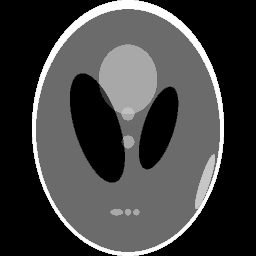
\includegraphics[width=0.8\textwidth]{Figuras/SL_rasterizado_EQ.png}
           \caption{Fantoma rasterizado y ecualizado.}
           \label{fig:SL_EQ}
        \end{subfigure}
   \caption{Fantoma de shepp-Logan rasterizado (a) y luego ecualizado (b).}
   \label{fig:SL}
\end{figure}

\subsection{Proyecciones del fantoma}

Se generaron proyecciones del fantoma Shepp-Logan utilizando los valores default del programa $\verb|CTSim|$. Estos valores son 367 detectores, 320 ángulos de proyección y 2 muestras por detector. De esta manera, se obtiene el sinograma que se muestra en la Fig. \ref{fig:SL_sinogram}, donde el eje horizontal representa los detectores y el eje vertical el ángulo de proyección.

\begin{figure}[H]
   \centering
         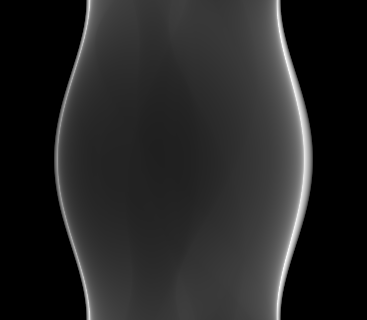
\includegraphics[width=0.5\textwidth]{Figuras/SL_sinogram.png}
   \caption{Sinograma del fantoma Shepp-Logan.}
   \label{fig:SL_sinogram}
\end{figure}

\subsection{Error de reconstrucción del fanotoma}

El error de reconstrucción se calcula como la diferencia cuadrática media entre la imagen original y la imagen reconstruida de dimensiones $N\times M$, es decir
\begin{equation}
      \text{Error} = \sqrt{\frac{1}{NM}\sum_{x,y}(g(x,y) - f(x,y))^2}
\end{equation}
donde $g(x,y)$ es la imagen original y $f(x,y)$ es la imagen reconstruida. En este trabajo, se normalizará la media de las imágenes antes de calcular el error de reconstrucción.

Se reconstruyó el fantoma Shepp-Logan utilizando retroproyección filtrada con filtro rampa a partir del sinograma de la Fig. \ref{fig:SL_sinogram} y se ecualizó la imagen obtenida para ampliar su rango dinámico. El error de reconstrucción obtenido entre la imagen original ecualizada y la imagen reconstruida ecualizada fue de $0.746177$. La imagen original, la reconstrucción y la diferencia entre ambas se muestran en la Fig. \ref{fig:sustraction}.

\begin{figure}[H]
   \centering
        \begin{subfigure}[h]{0.32\linewidth}
           \centering
           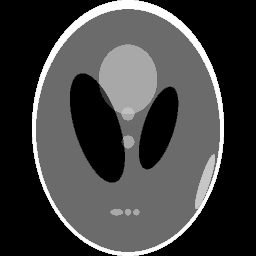
\includegraphics[width=\textwidth]{Figuras/SL_rasterizado_EQ.png}
           \caption{Imagen original.} 
           \label{fig:original}
        \end{subfigure}
        \begin{subfigure}[h]{0.32\linewidth}
           \centering
           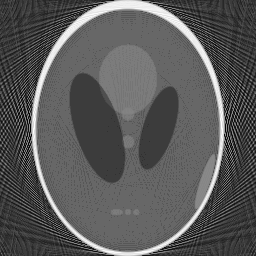
\includegraphics[width=\textwidth]{Figuras/SL_rec_lineal_EQ.png}
           \caption{Retroproyección filtrada.}
           \label{fig:reconstruccion}
        \end{subfigure}
        \begin{subfigure}[h]{0.32\linewidth}
         \centering
         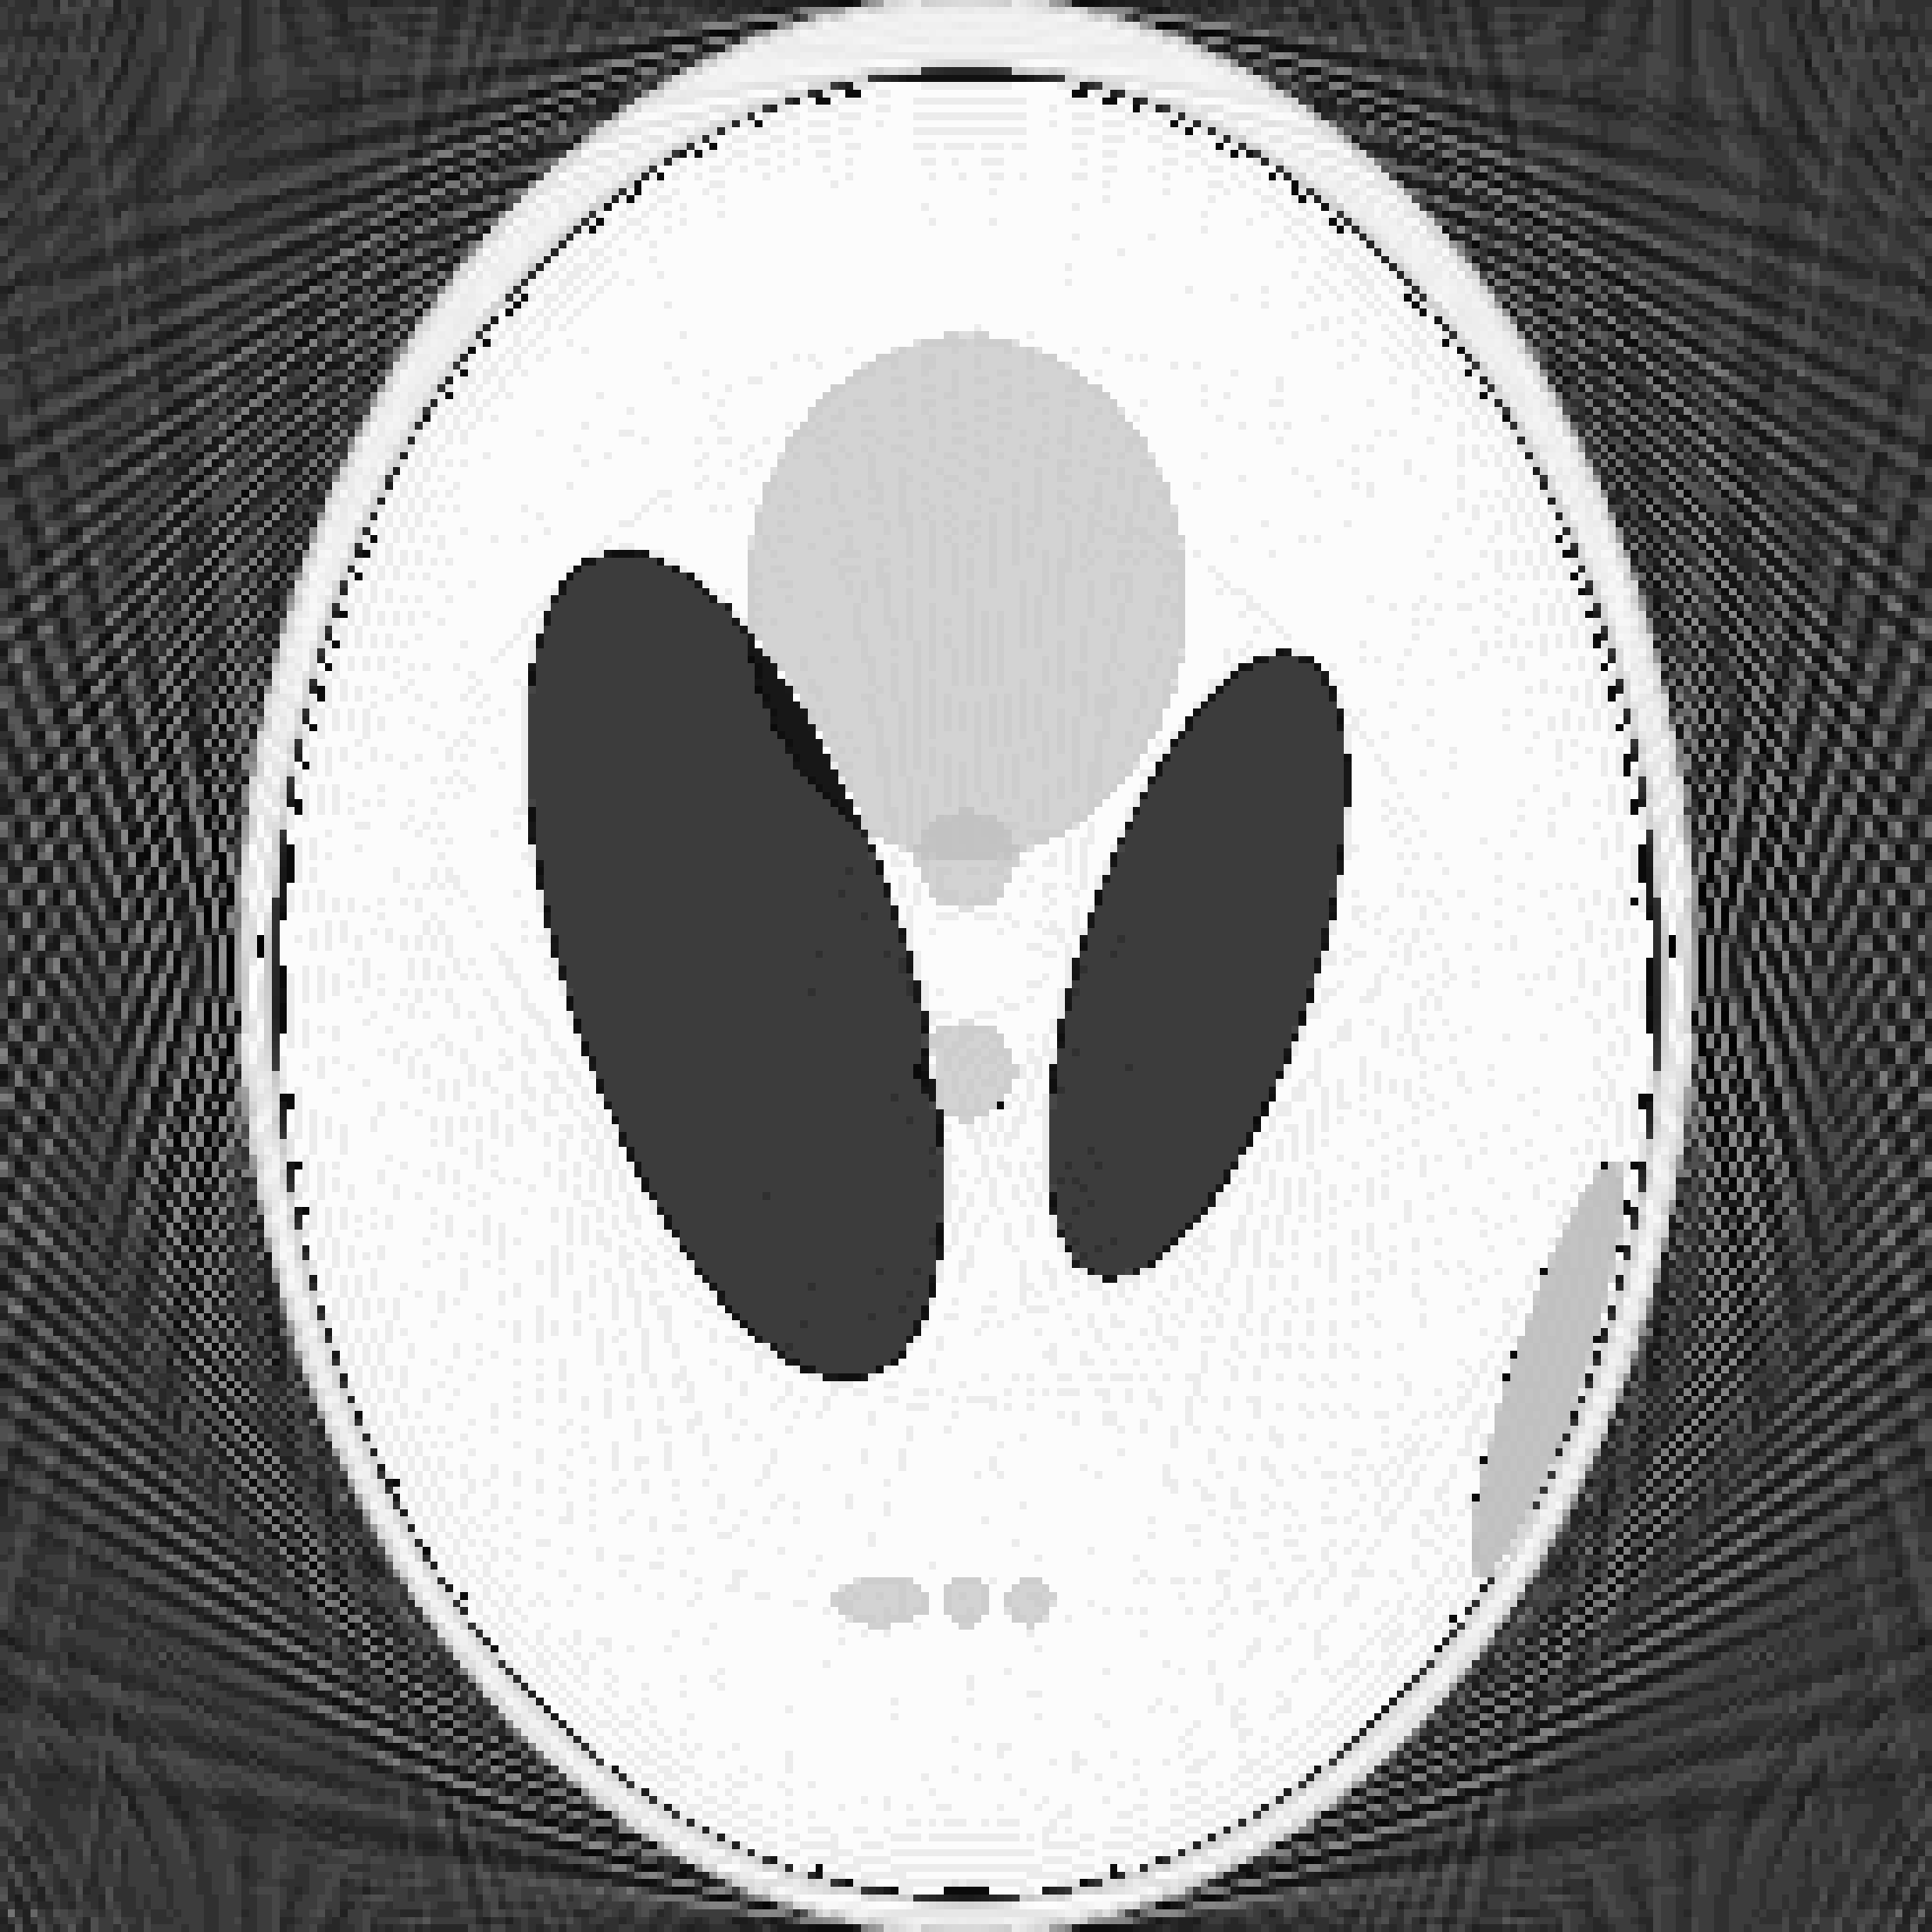
\includegraphics[width=\textwidth]{Figuras/sustraction.png}
         \caption{Diferencia entre (b) y (a).}
         \label{fig:resta}
      \end{subfigure}
   \caption{(a) Fantoma de Shepp-Logan original ecualizad. (b) Reconstrucción por retroproyección con filtro rampa a partir del sinograma de la Fig. \ref{fig:SL_sinogram} y ecualizado. (c) Diferencia entre la imagen reconstruida y la original.}
   \label{fig:sustraction}
\end{figure}

\section{Error de reconstrucción en función de parámetros de adquisición y reconstrucción}

Se estudió el error de reconstrucción como función del número de detectores, y número de proyecciones (parámetros de adquisión) y del tipo de filtros (parámetro de reconstrucción). Para esto, se generaron fantomas de Shepp-Logan en $\verb|python|$ utilizando como base el programa \\$\verb|radon-skimage.py|$ provisto. 

En primer lugar, se varió el número de detectores entre 25 y 1000, en intervalos de a 25, y se utilizaron con 320 proyecciones con filtro rampa. Por otro lado, se varío el número de proyecciones entre 20 y 800, en intervalos de 20, y se utilizaron 367 detectores y filtro rampa. Por último, se varió el tipo de filtro entre rampa, Hamming, Hanning y coseno con 367 detectores y 320 proyecciones. El comportamiento del error de reconstrucción en función de los parámetros mencionados se muestra Fig. \ref{fig:err_vs_param}.

\begin{figure}[H]
   \centering
        \begin{subfigure}[h]{0.32\linewidth}
           \centering
           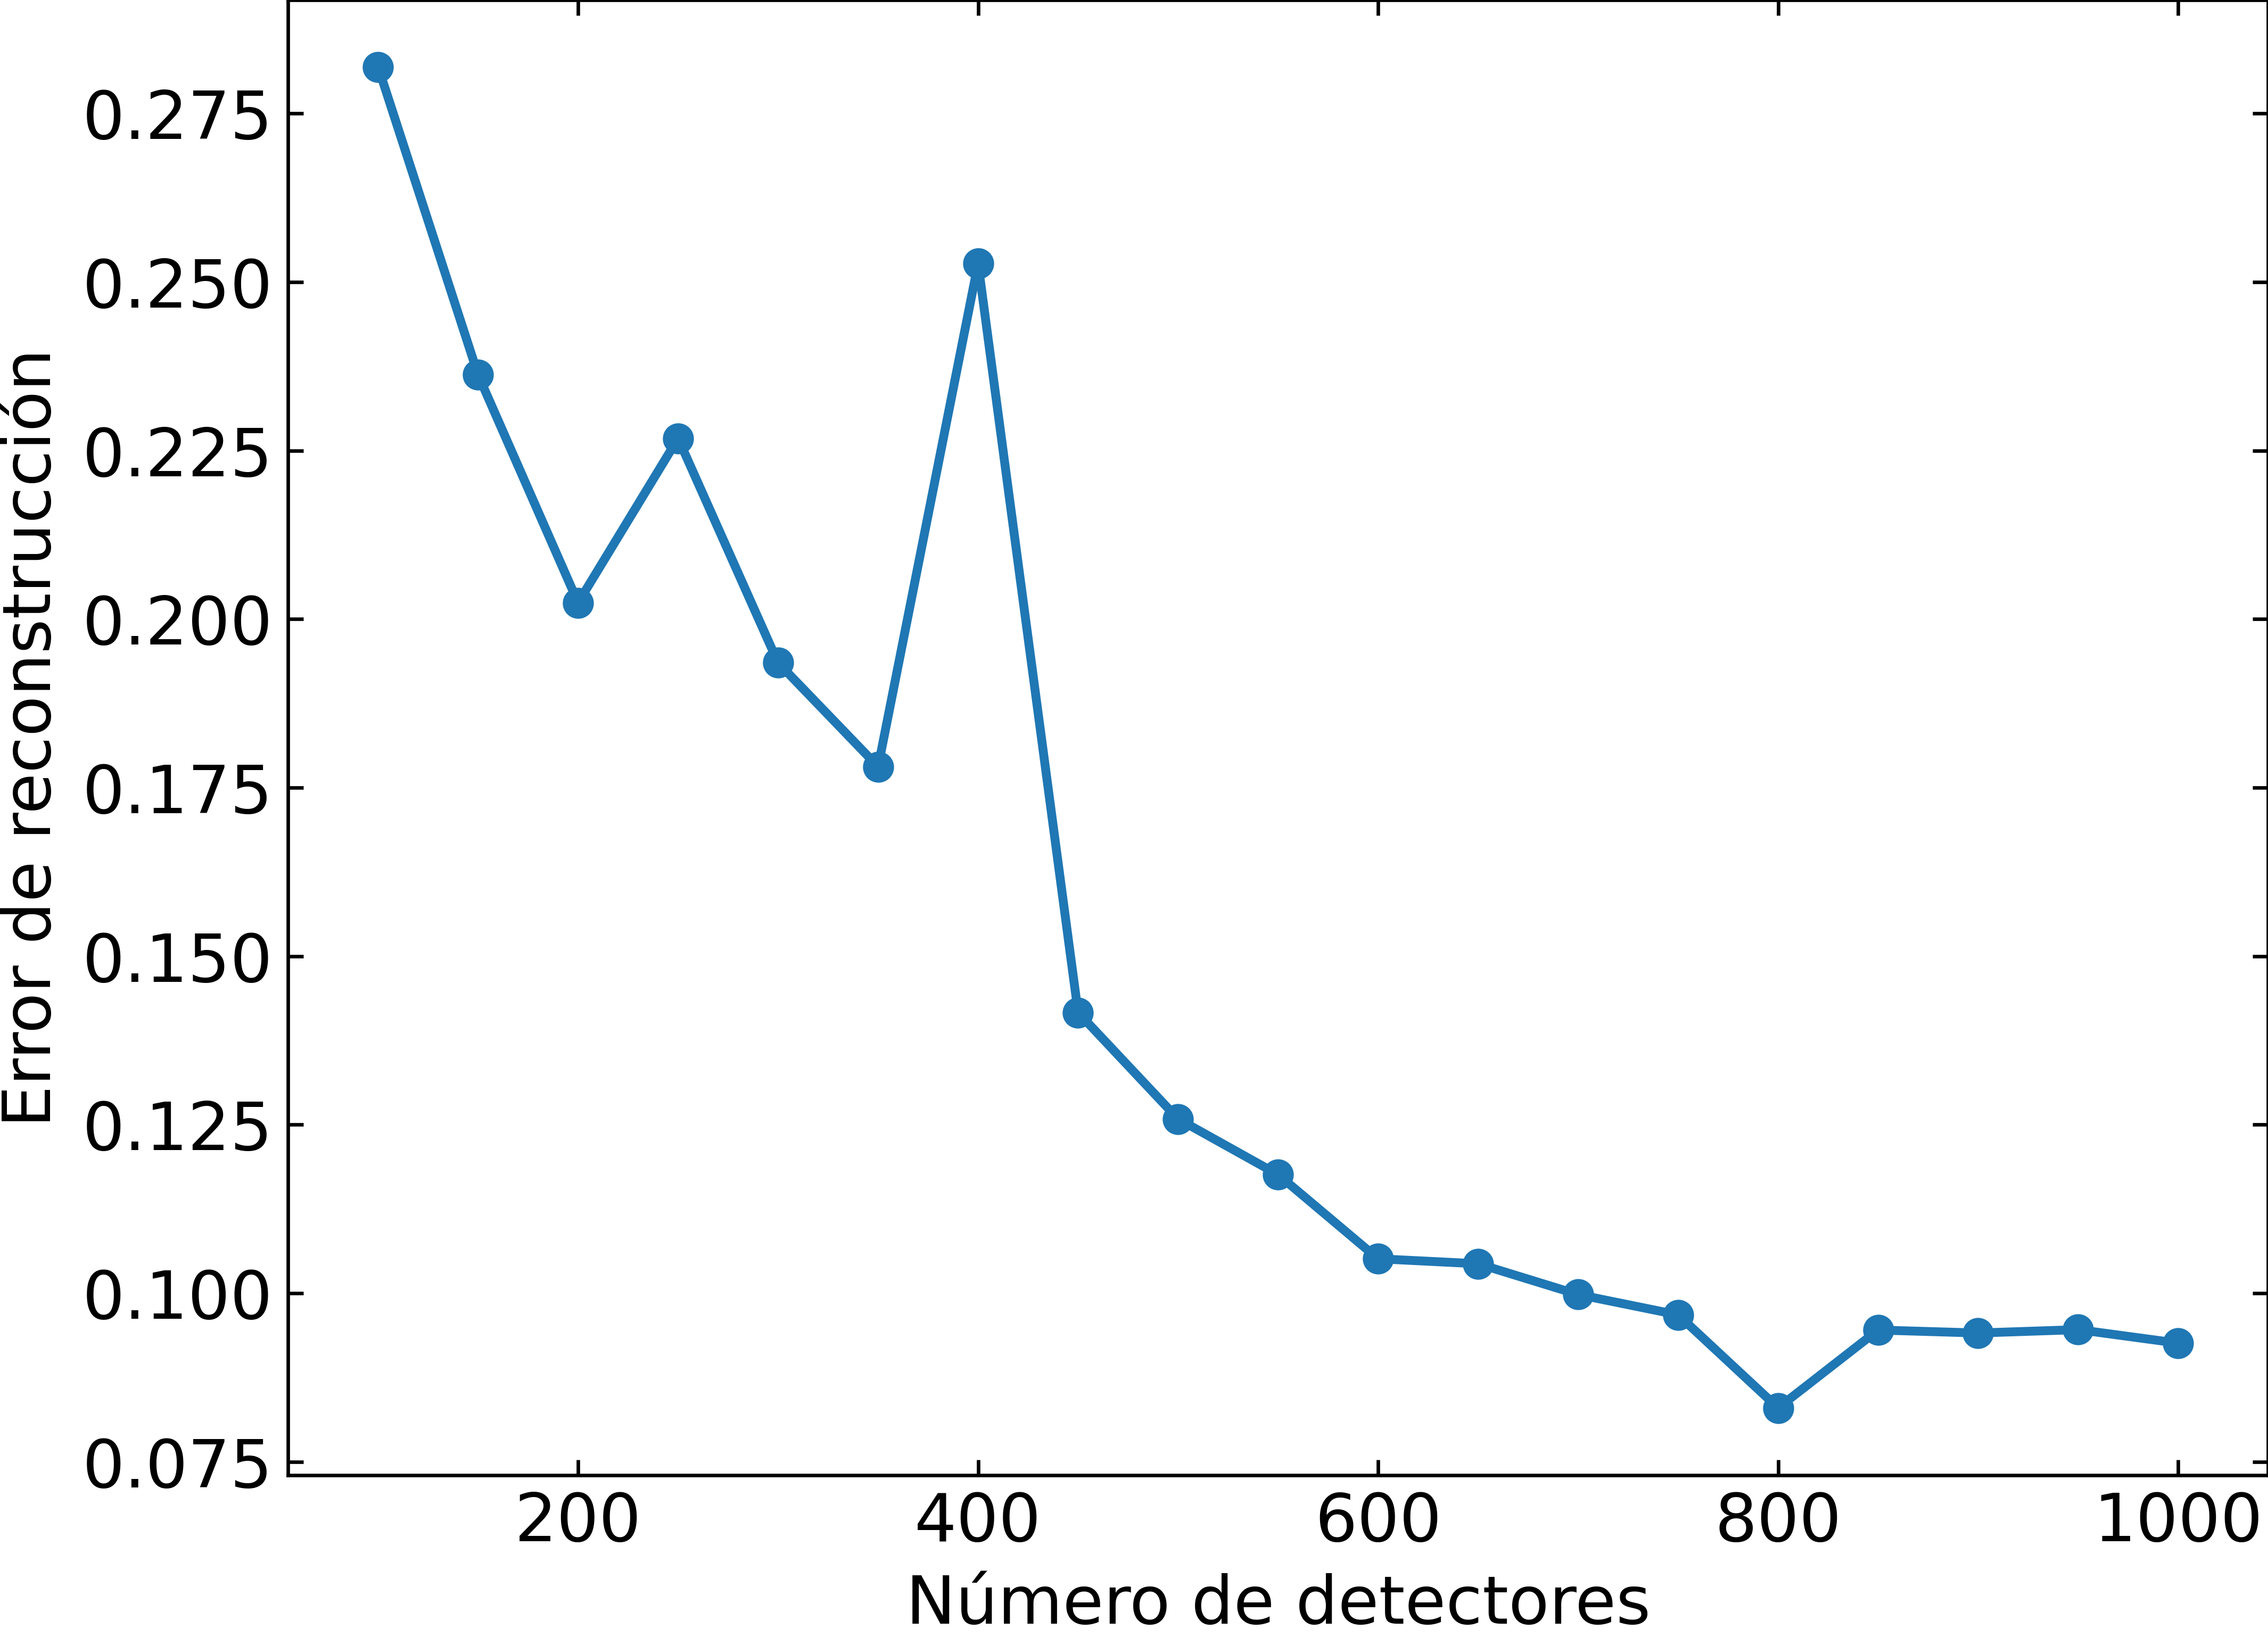
\includegraphics[width=\textwidth]{Figuras/error_vs_detectores.png}
           \caption{} 
           \label{fig:err_det}
        \end{subfigure}
        \begin{subfigure}[h]{0.32\linewidth}
           \centering
           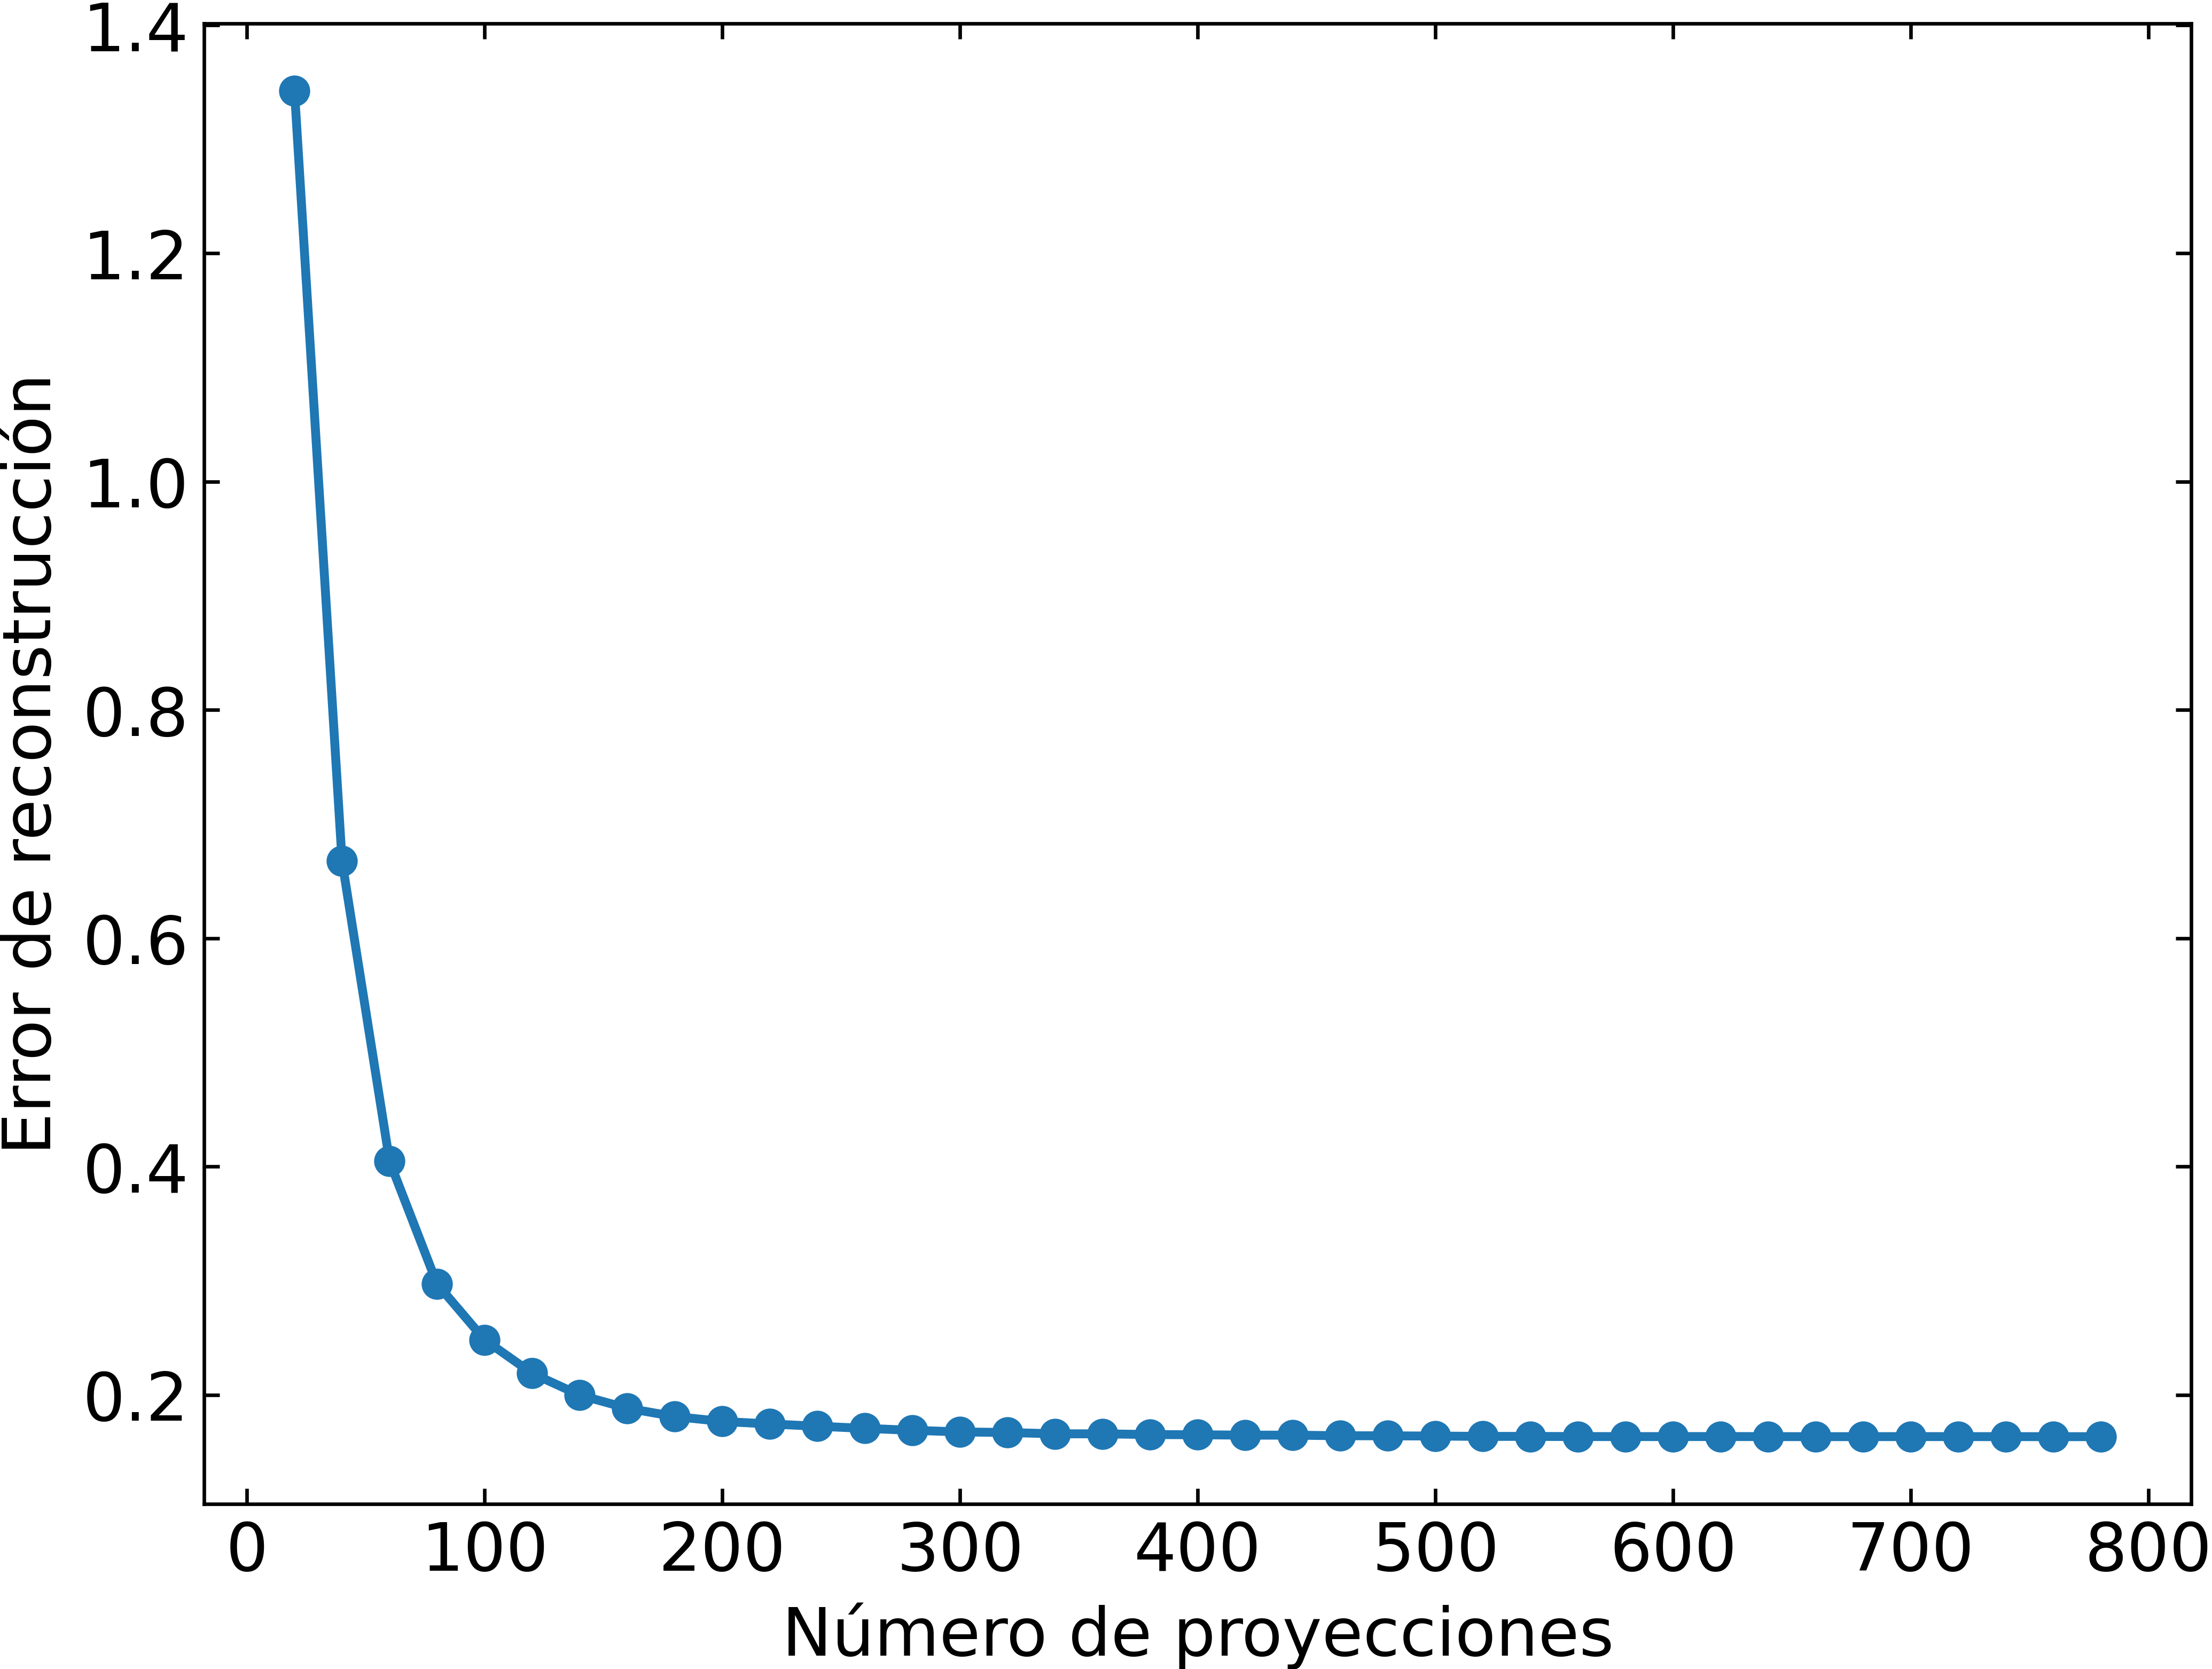
\includegraphics[width=\textwidth]{Figuras/error_vs_proyecciones.png}
           \caption{}
           \label{fig:err_proy}
        \end{subfigure}
        \begin{subfigure}[h]{0.32\linewidth}
         \centering
         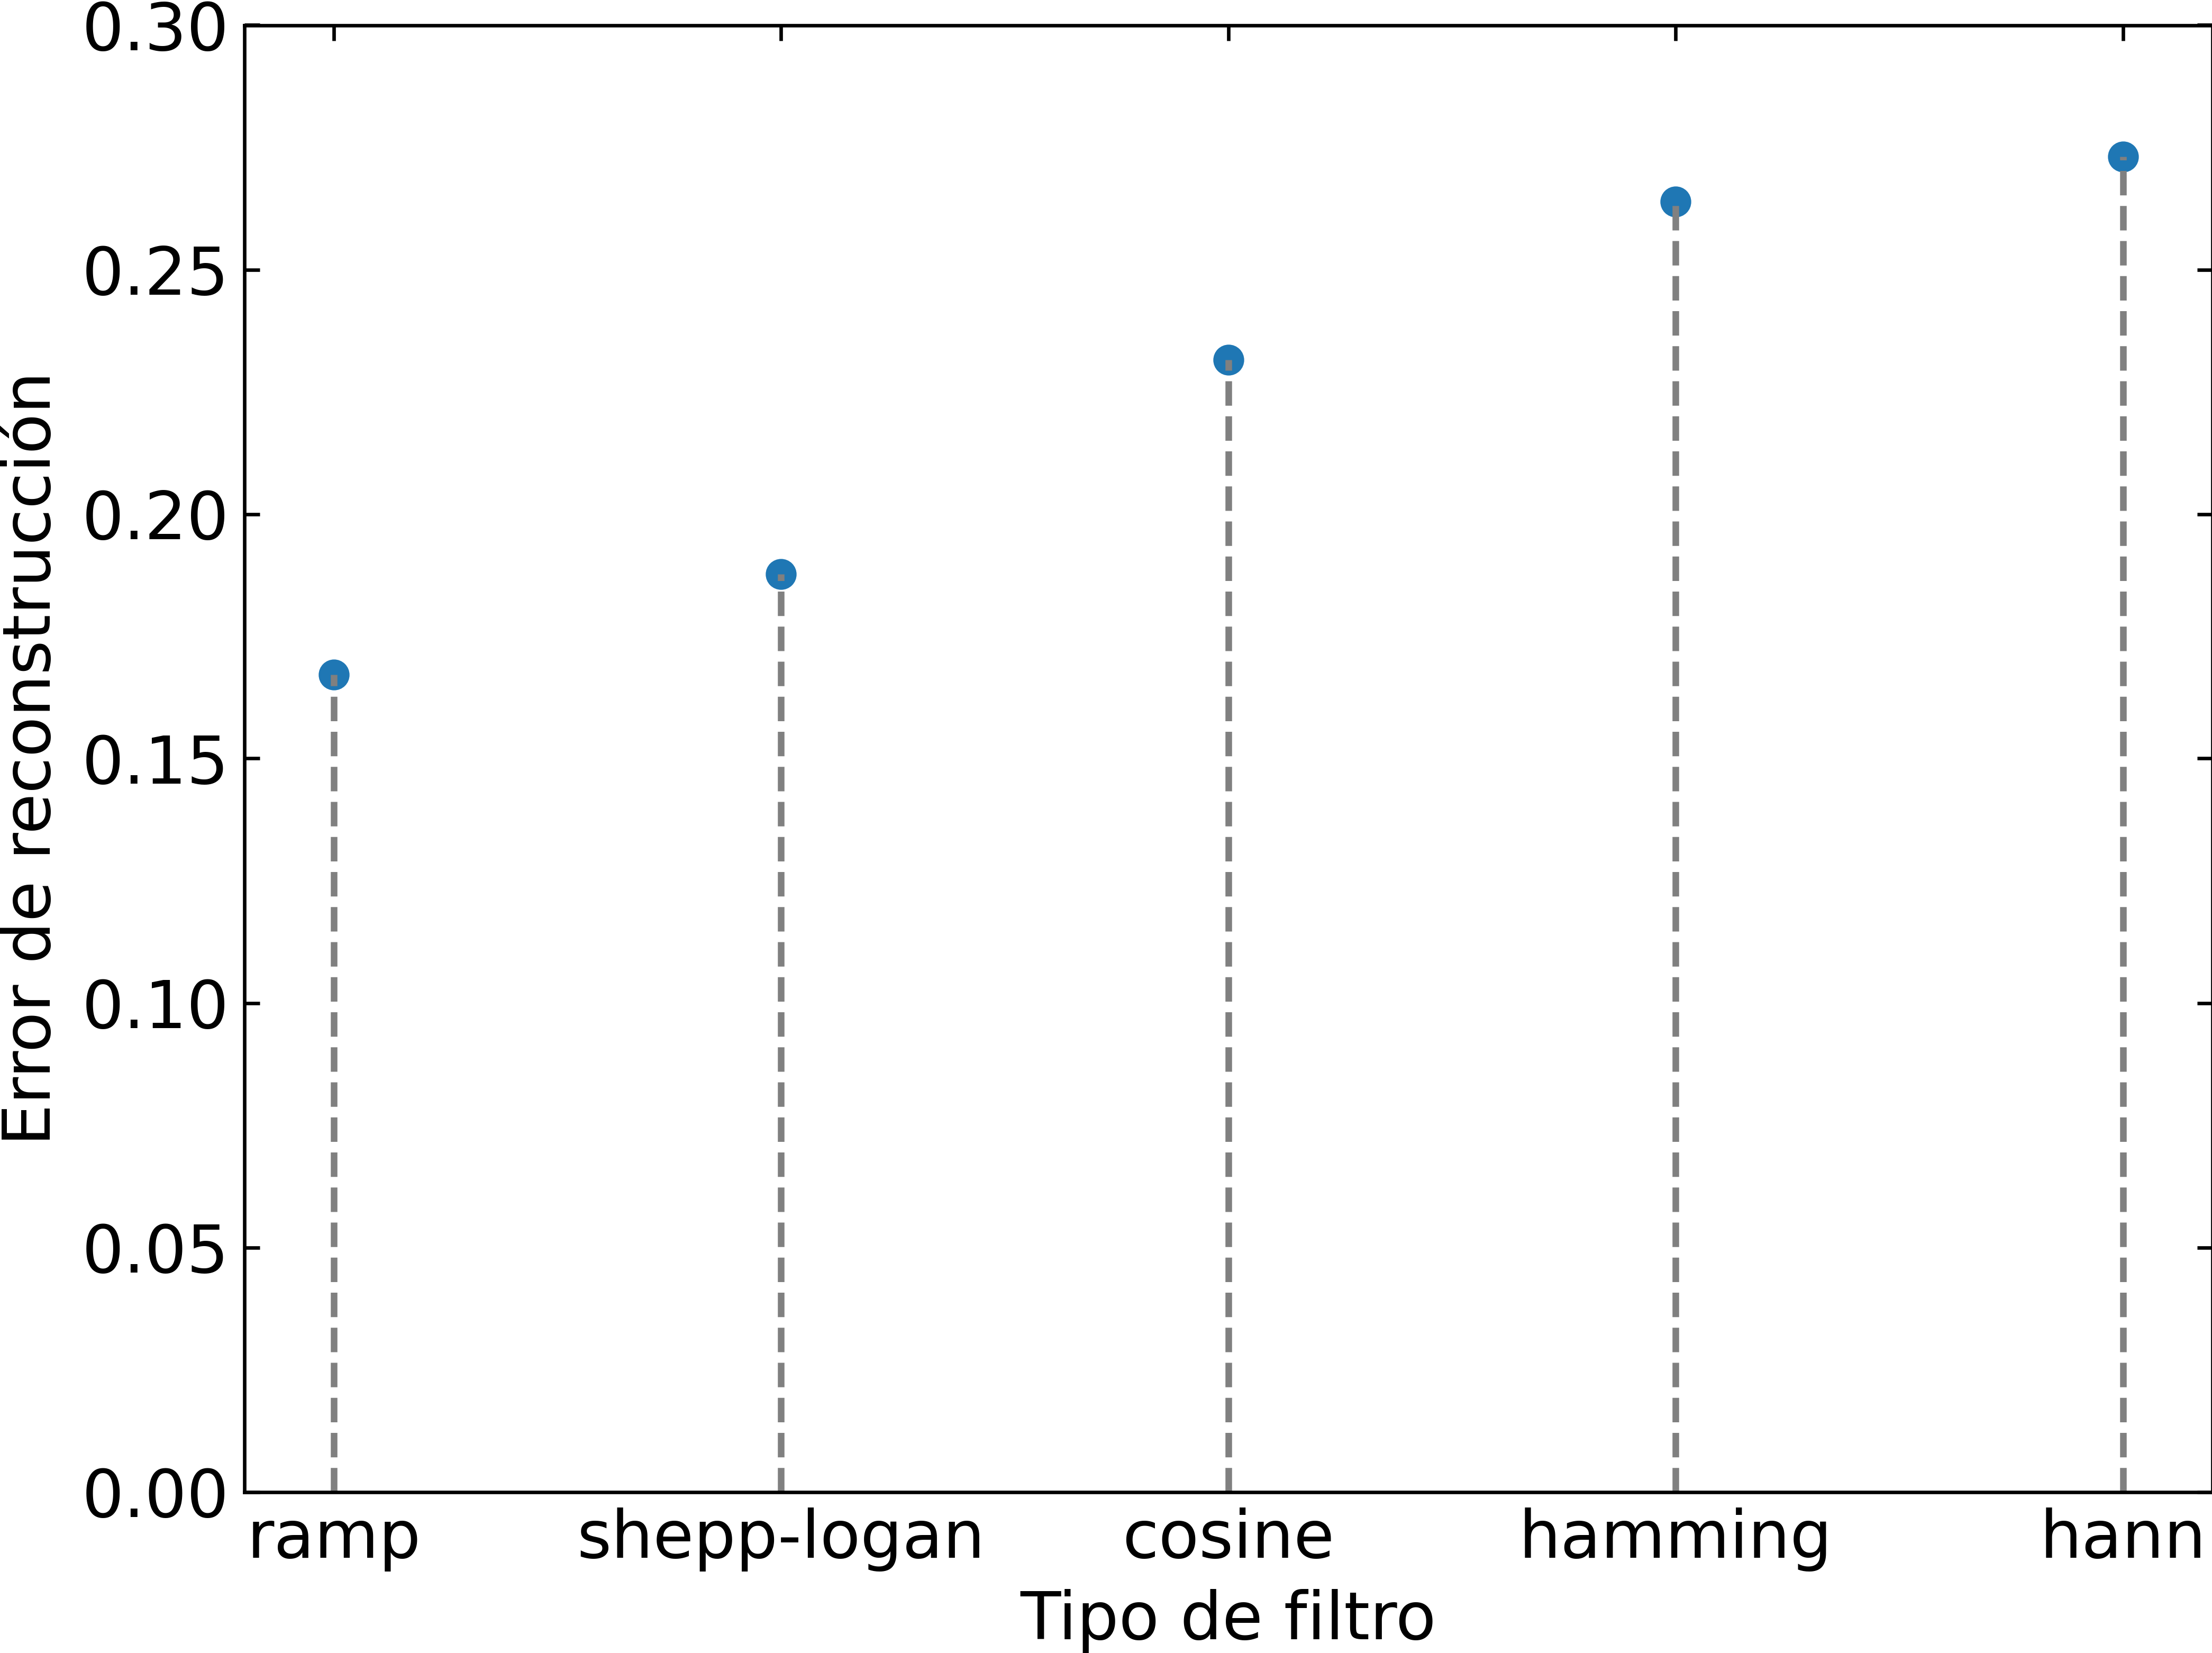
\includegraphics[width=\textwidth]{Figuras/error_vs_filters.png}
         \caption{}
         \label{fig:err_filtro}
      \end{subfigure}
   \caption{Errores de reconstrucción en función del número de detectores (a), número de proyecciones (b) y tipo de filtro (c).}
   \label{fig:err_vs_param}
\end{figure}

En general, se observa que al aumentar el número de detectores y proyecciones, el error de reconstrucción disminuye. En particular, aumentar el número de proyecciones disminuye muy rápidamente el error de reconstrucción y llega a un valor estacionario en 200 proyecciones aproximadamente. Además, en este caso de un fantoma Shepp-Logan sin ruido, se observa que el filtro que mejor reconstrucción produce es el filtro rampa. 

\section{Sinograma de Shepp-Logan con ruido}

En esta sección se estudiaron los efectos del ruido utilizando diversos filtros. Para esto, utilizando $\verb|numpy.random|$ se agregó ruido gaussiano al sinograma del fantoma Shepp-Loga obtenido con 367 detectores y 320 proyecciones (ver Fig. \ref{fig:SL_sinogram}) con desvío igual al $10\%$ del valor máximo del sinograma. Posteriormente, utilizando como base el programa $\verb|radon-skimage.py|$ provisto, se reconstruyó dicha imagen con retroproyección filtrada utilizando los filtros rampa, Hamming, Hanning y coseno. En la Fig. \ref{fig:noise_vs_filters} se muestran los resultados obtenidos. 

\begin{figure}[H]
   \centering
      \begin{subfigure}[h]{0.32\linewidth}
         \centering
         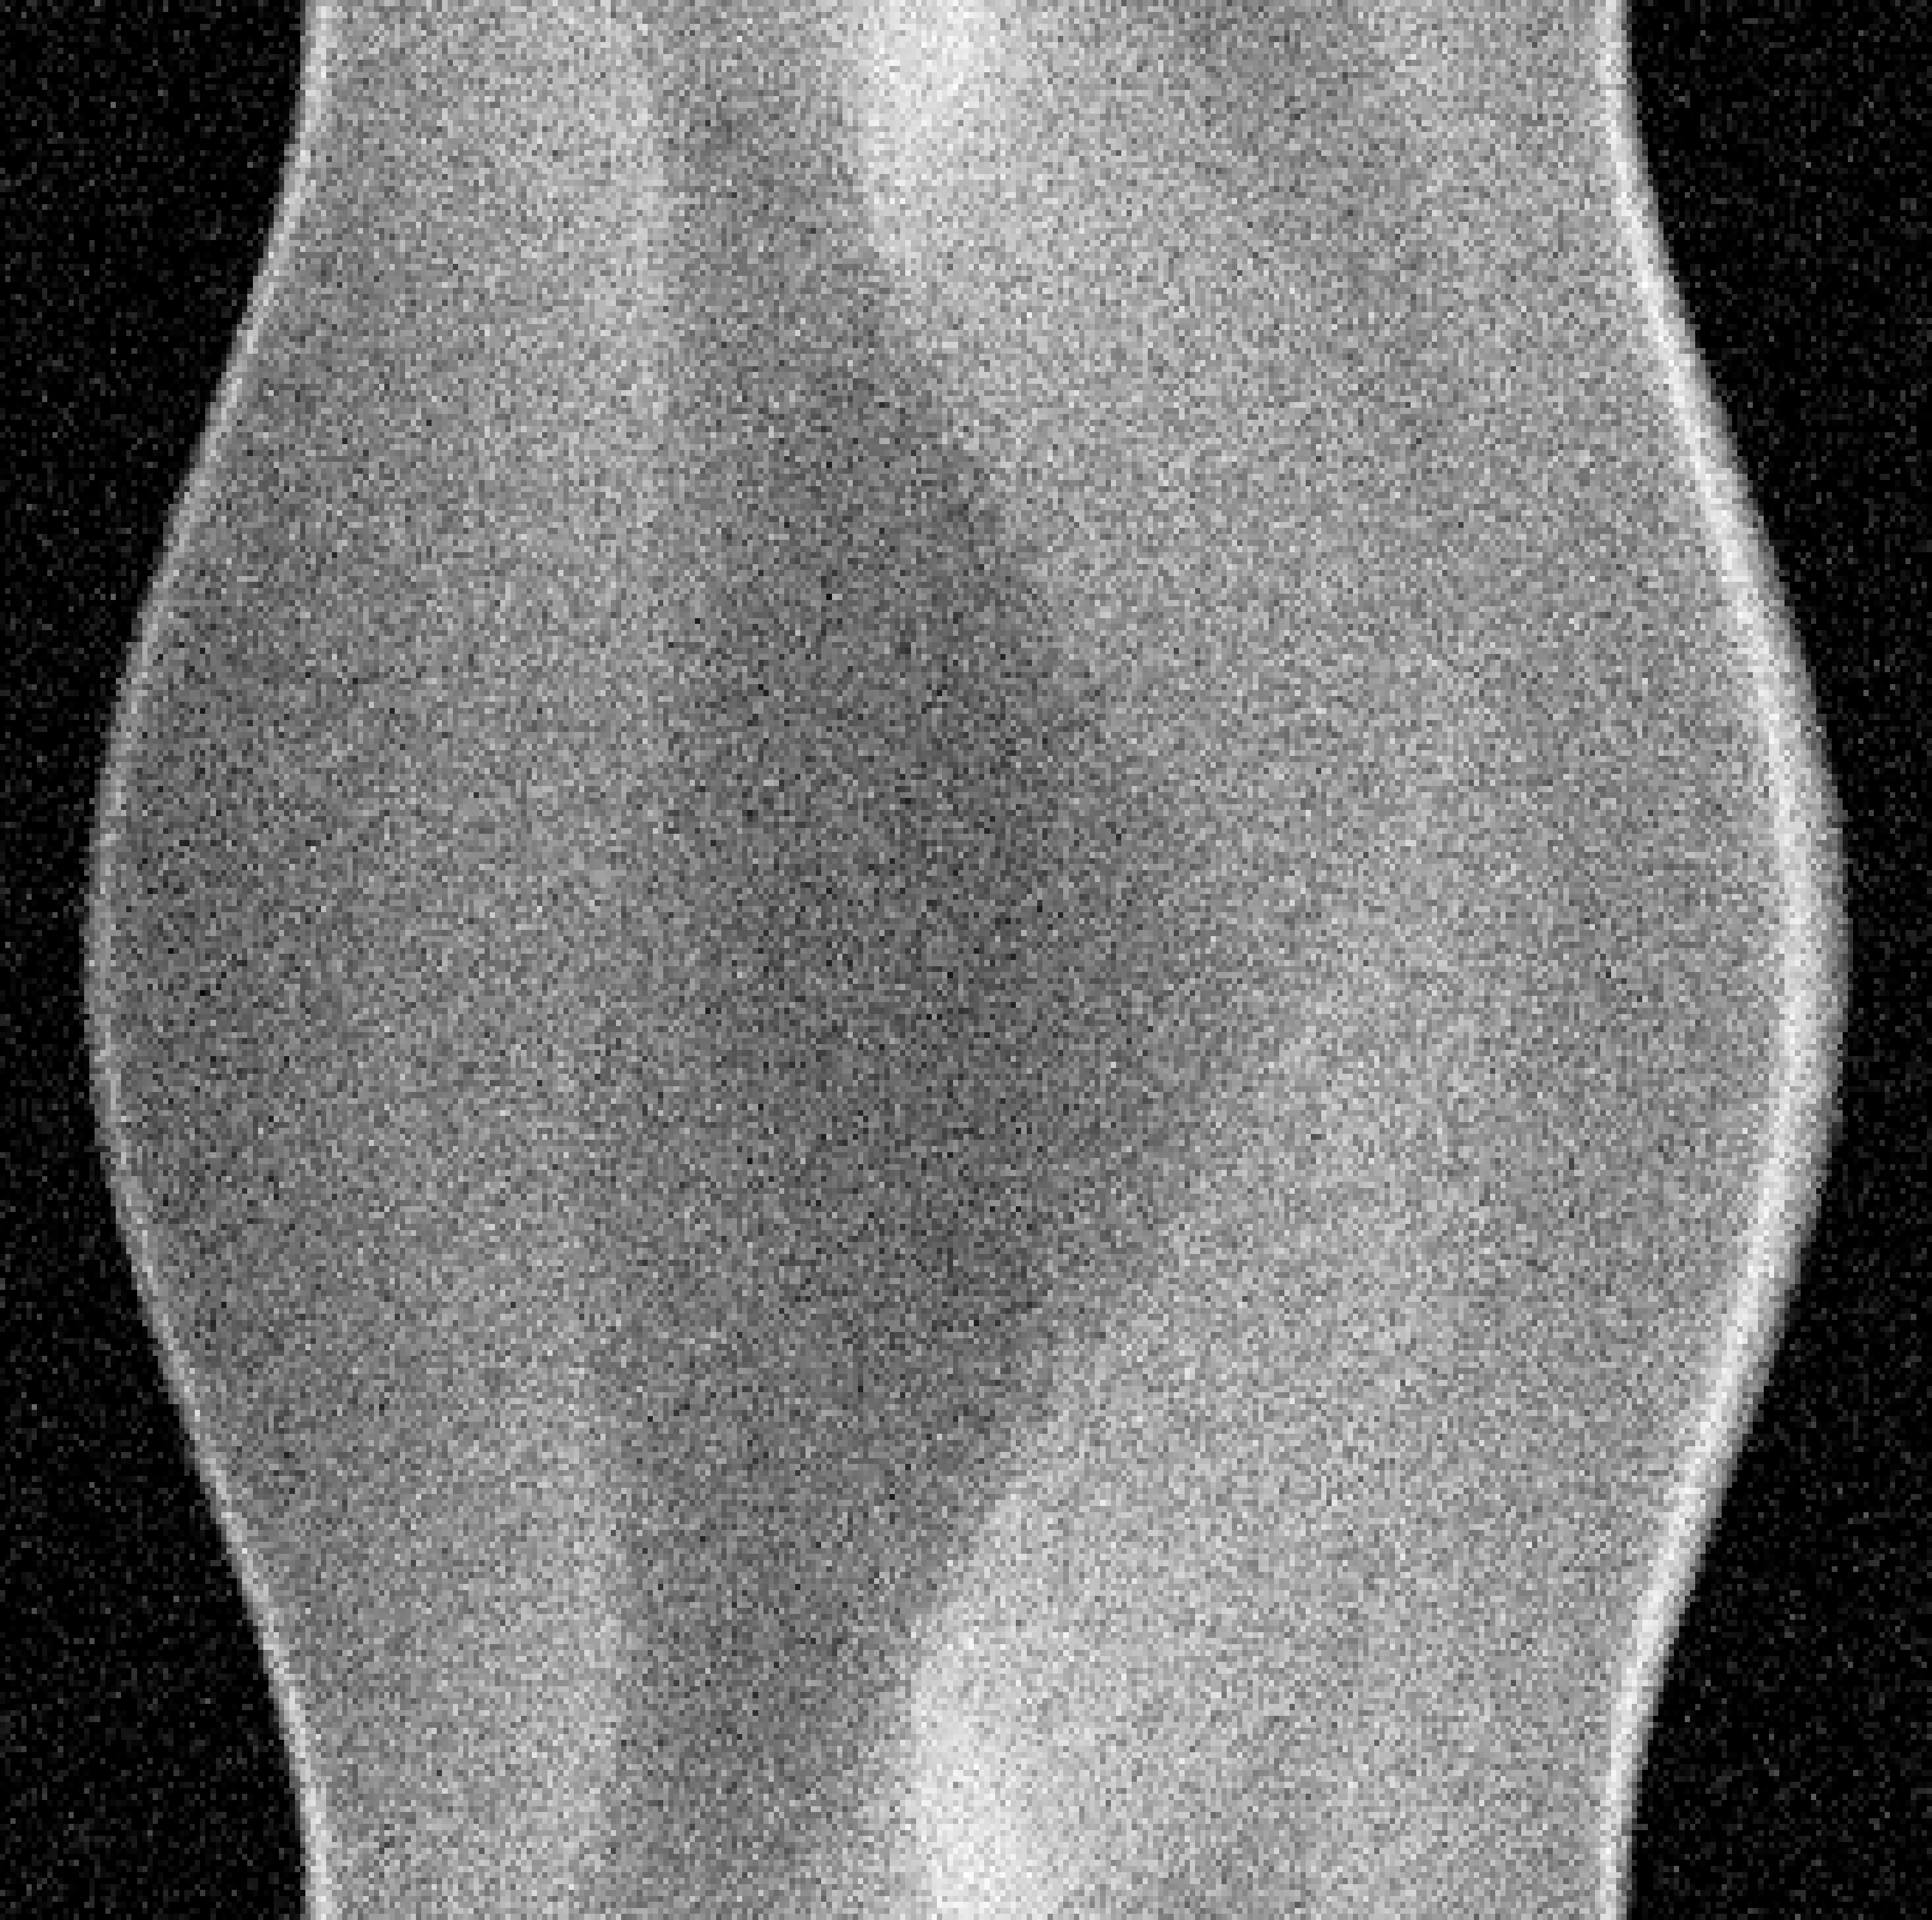
\includegraphics[width=\textwidth]{Figuras/sinograma_0.1.png}
         \caption{Sinograma con ruido.} 
         \label{fig:sinogram_0.1}
      \end{subfigure}
        \begin{subfigure}[h]{0.32\linewidth}
           \centering
           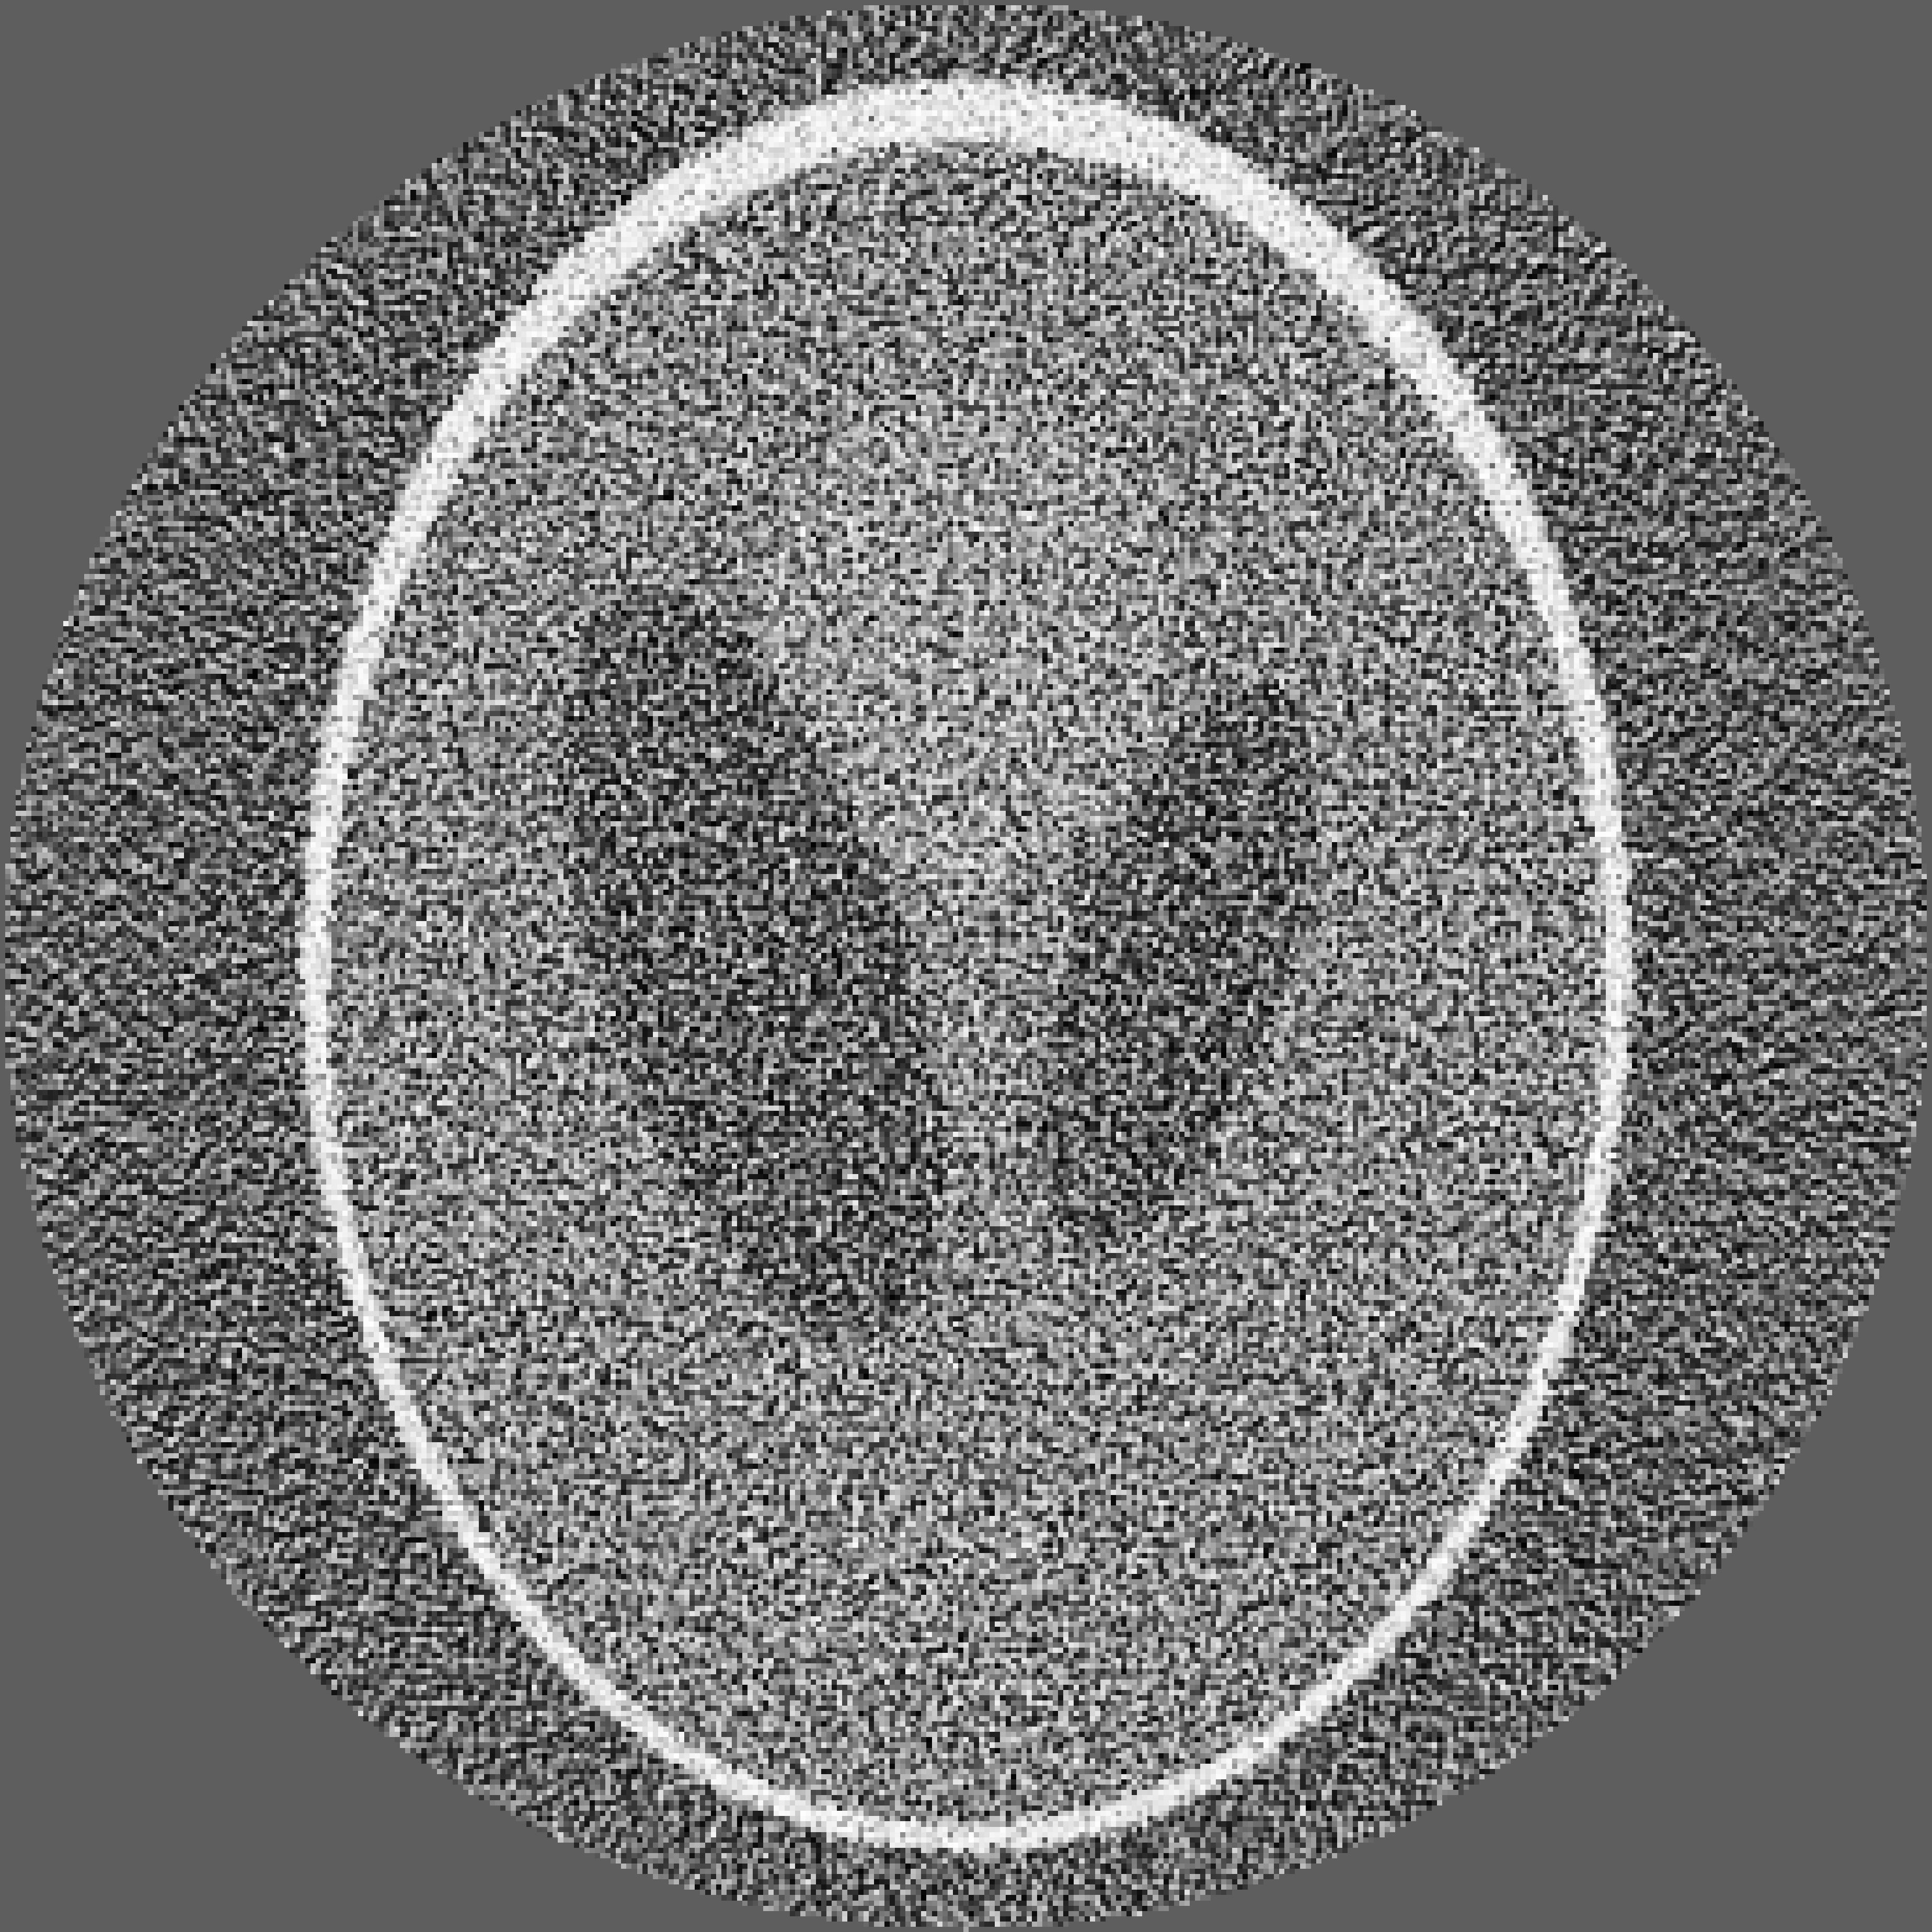
\includegraphics[width=\textwidth]{Figuras/reconstruction_ramp_EQ.png}
           \caption{Filtro rampa.} 
           \label{fig:noise_ramp}
        \end{subfigure}
        \begin{subfigure}[h]{0.32\linewidth}
           \centering
           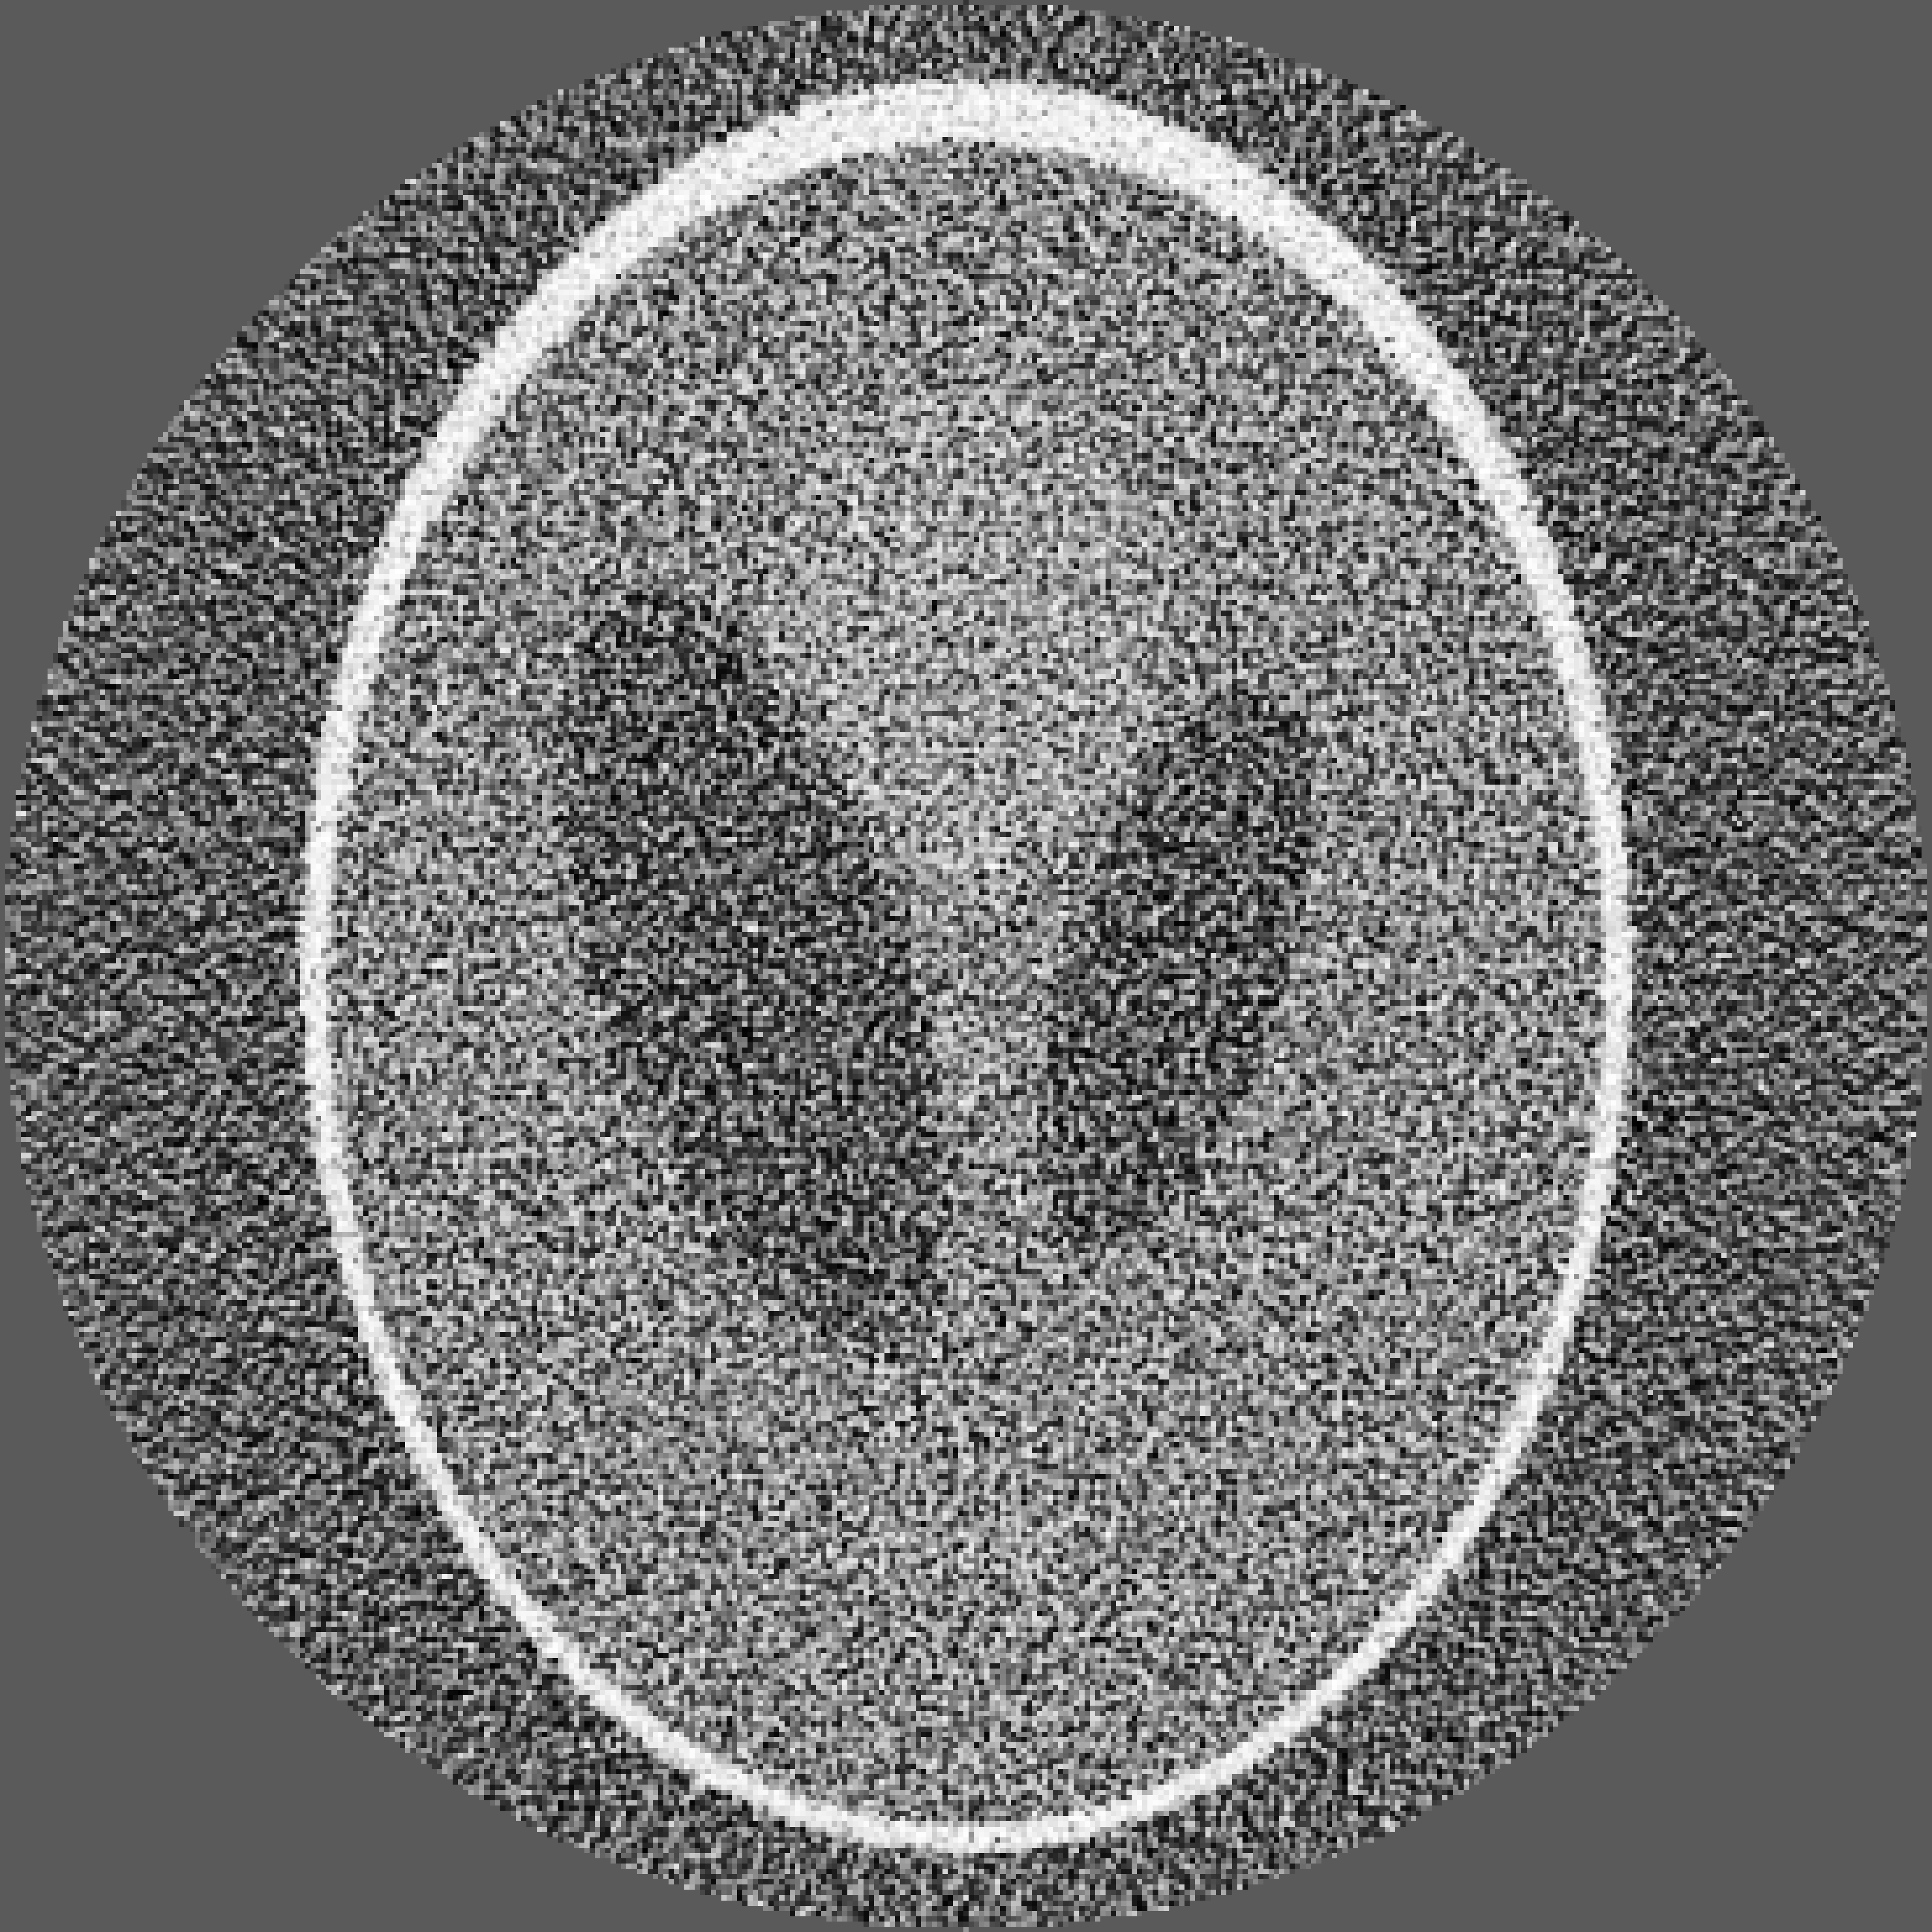
\includegraphics[width=\textwidth]{Figuras/reconstruction_shepp-logan_EQ.png}
           \caption{Filtro Shepp-Logan.}
           \label{fig:noise_shepp}
        \end{subfigure}
        \begin{subfigure}[h]{0.32\linewidth}
            \centering
            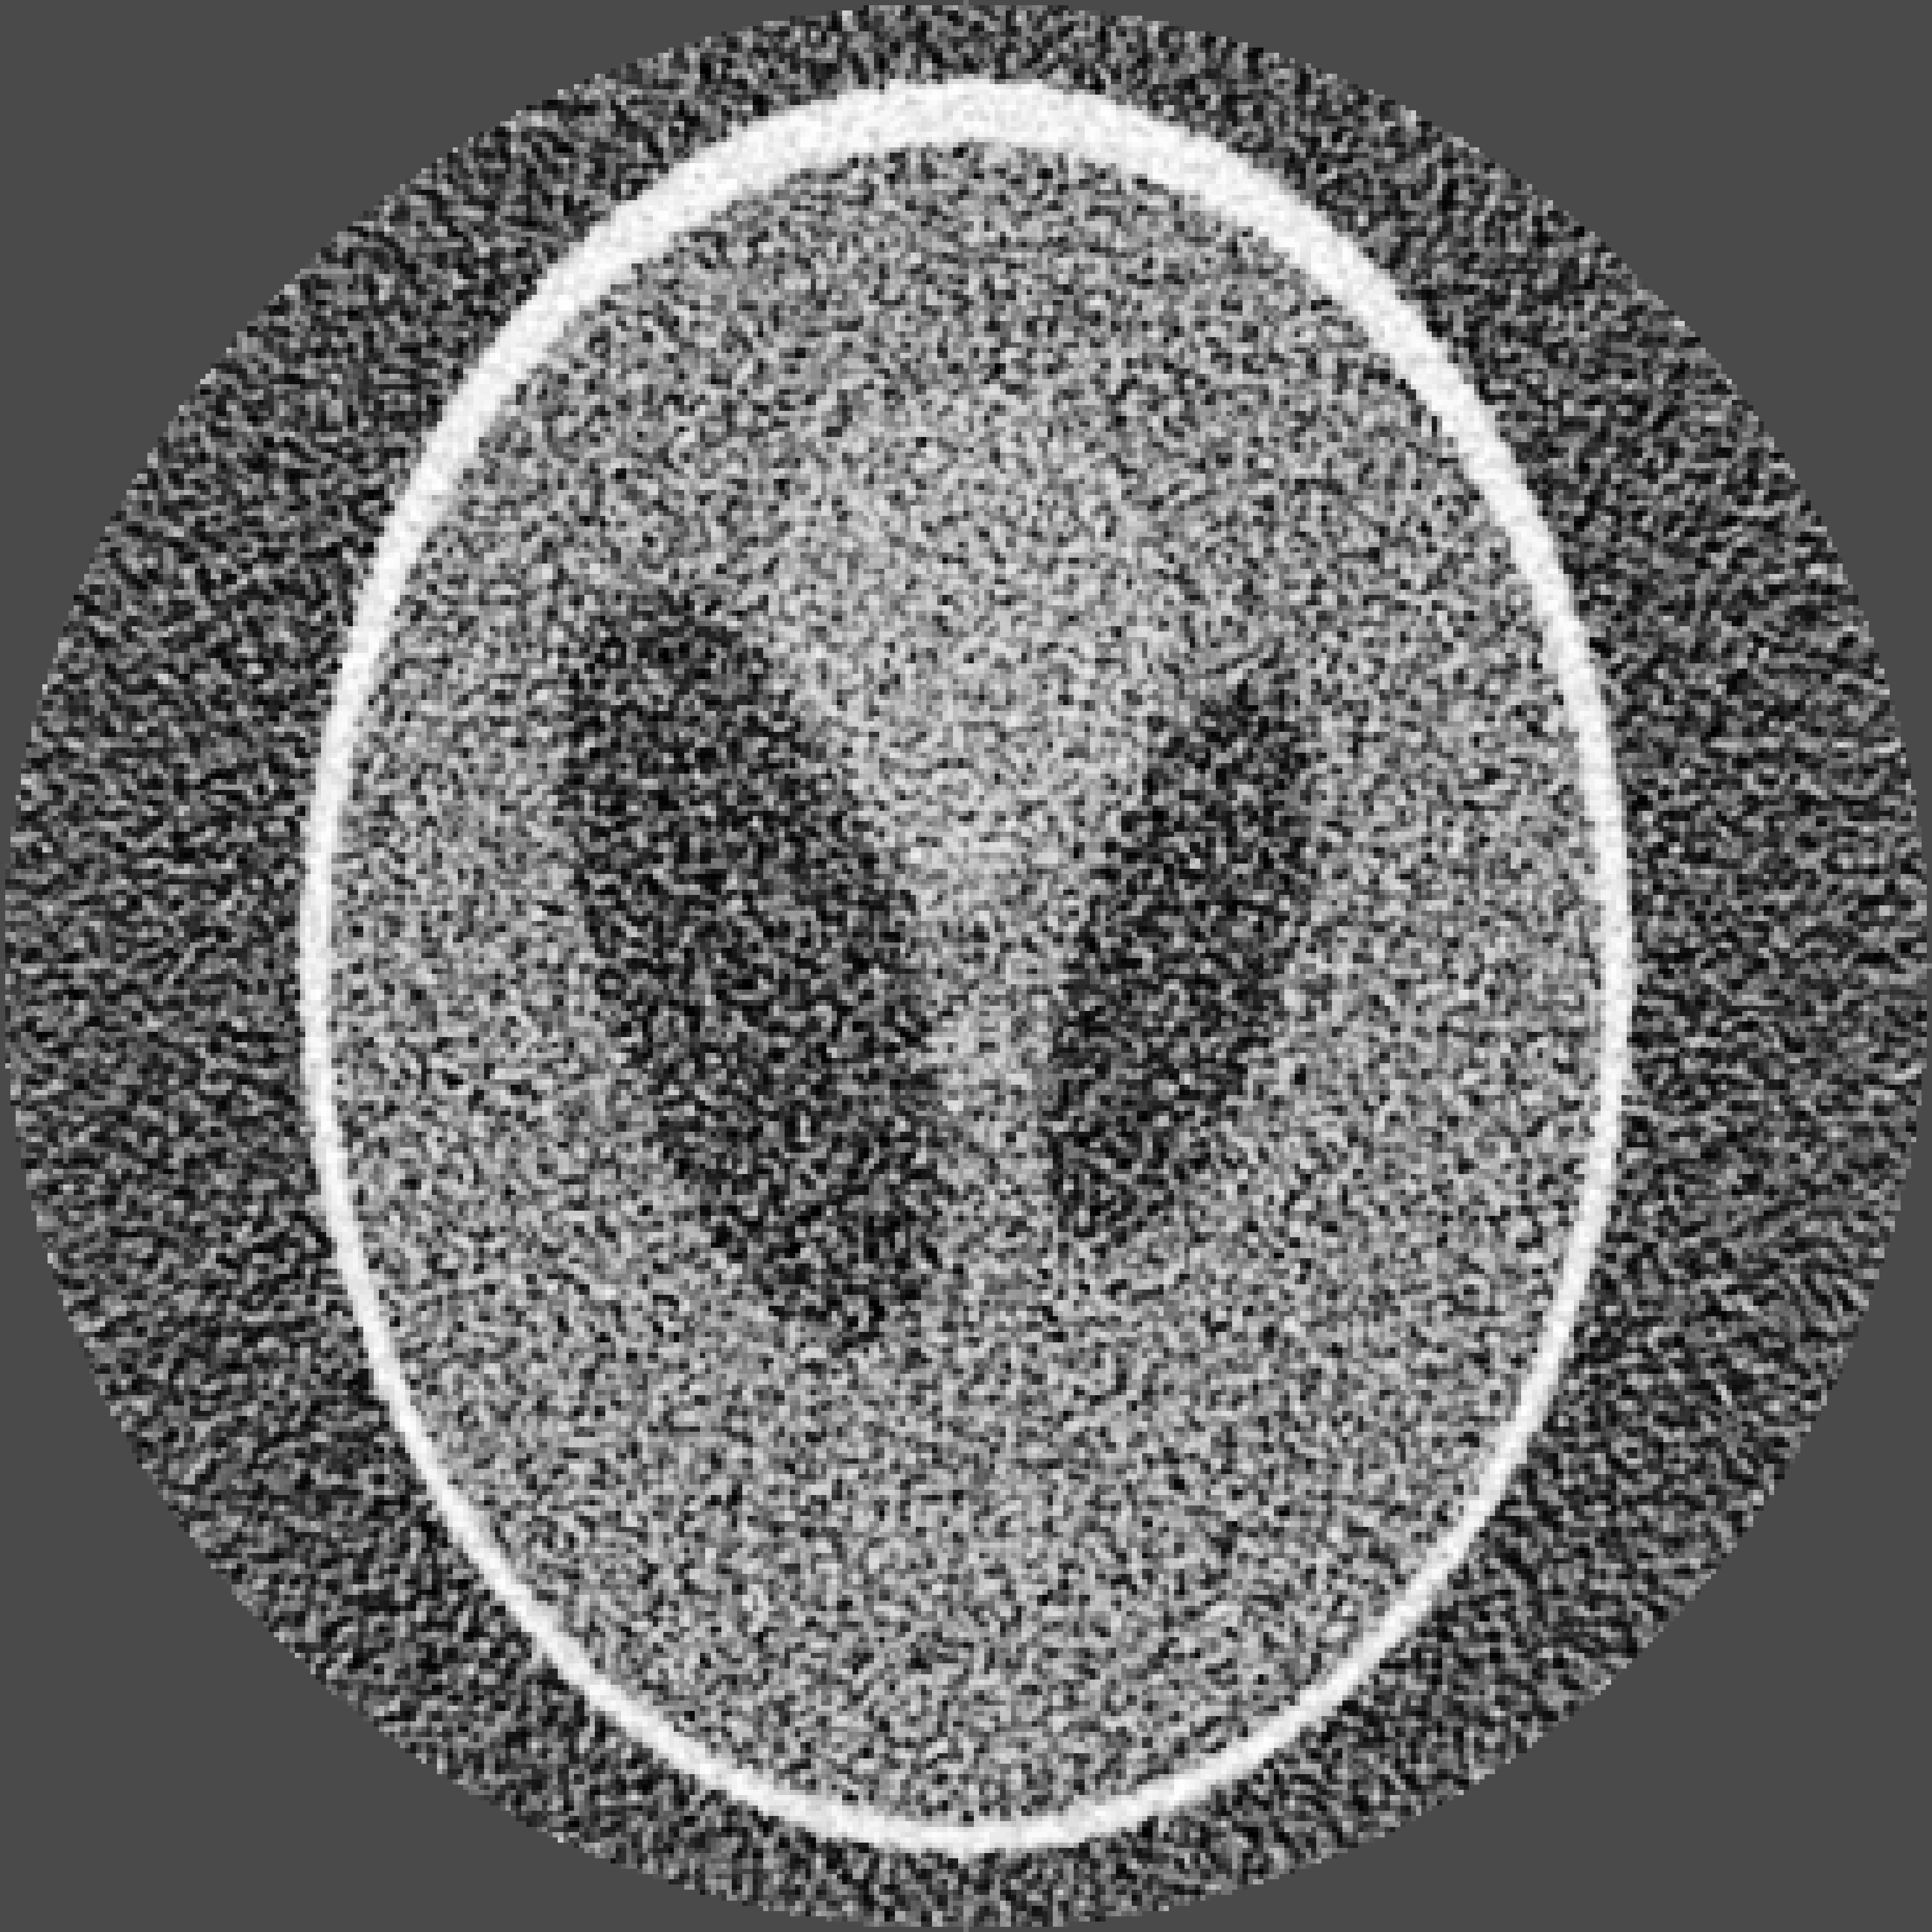
\includegraphics[width=\textwidth]{Figuras/reconstruction_cosine_EQ.png}
            \caption{Filtro coseno.}
         \label{fig:noise_coseno}
       \end{subfigure}
         \begin{subfigure}[h]{0.32\linewidth}
            \centering
            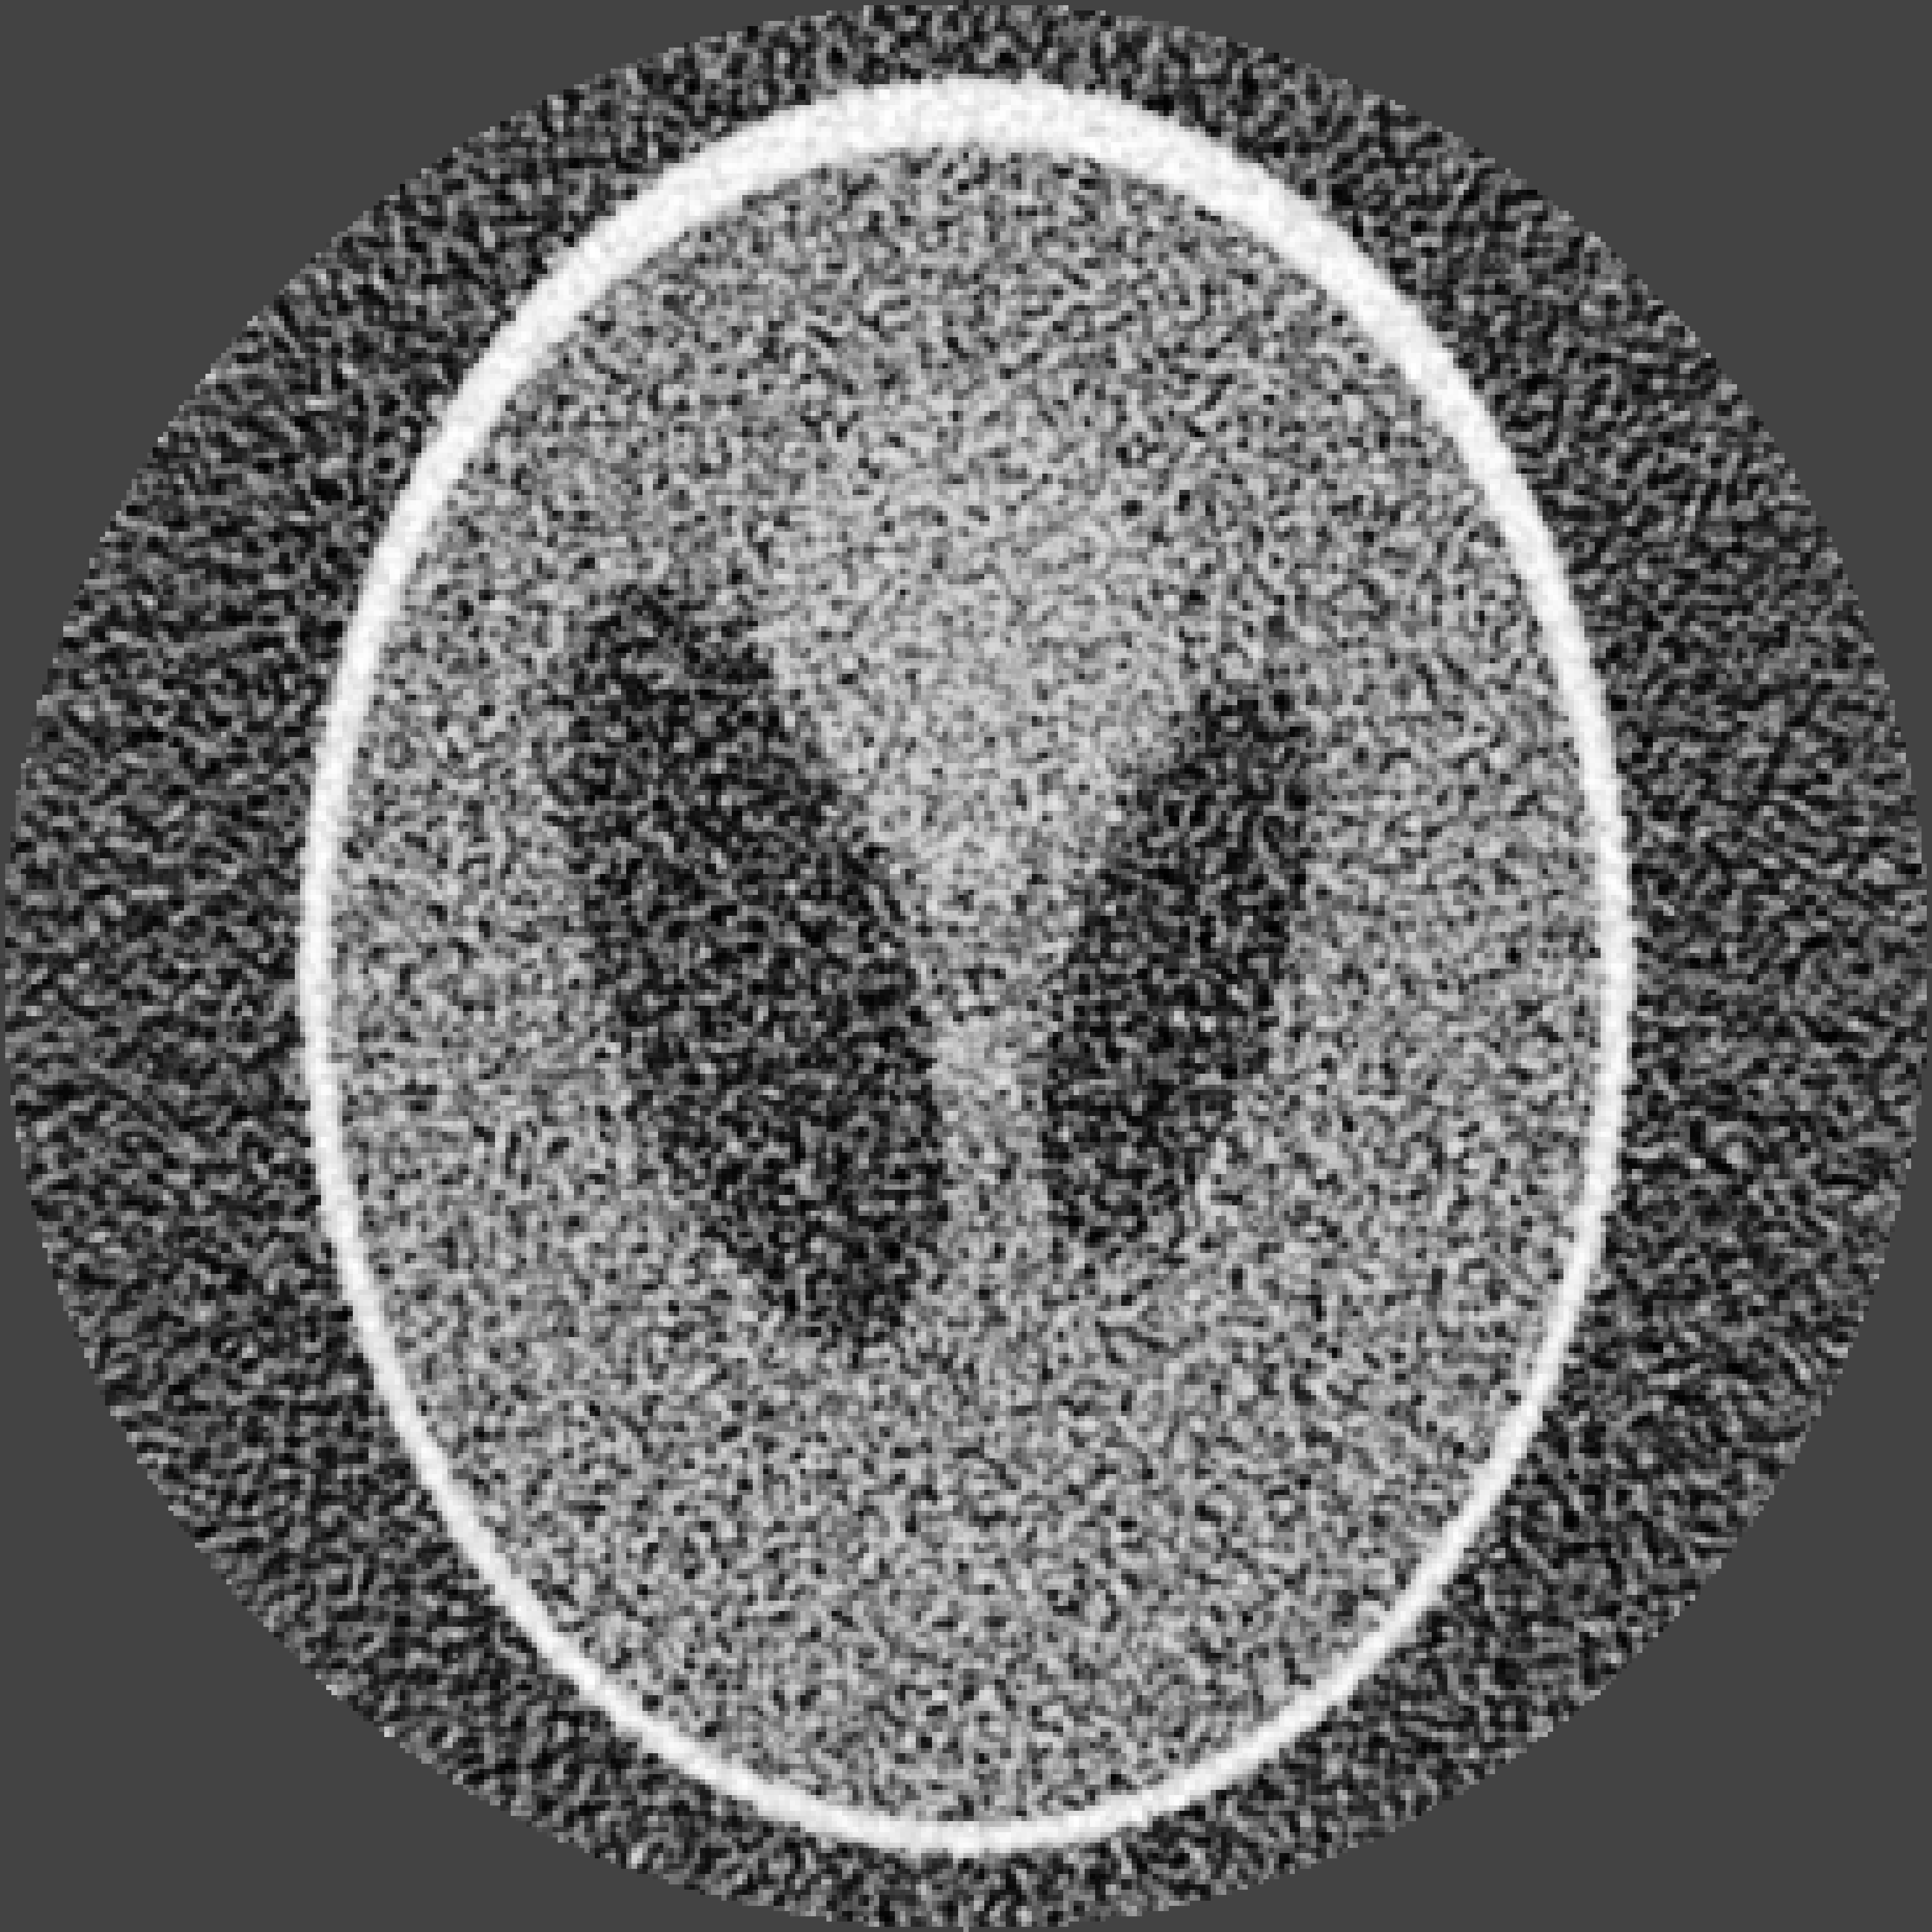
\includegraphics[width=\textwidth]{Figuras/reconstruction_hamming_EQ.png}
            \caption{Filtro Hamming.}
            \label{fig:noise_hamming}
         \end{subfigure}
         \begin{subfigure}[h]{0.32\linewidth}
            \centering
            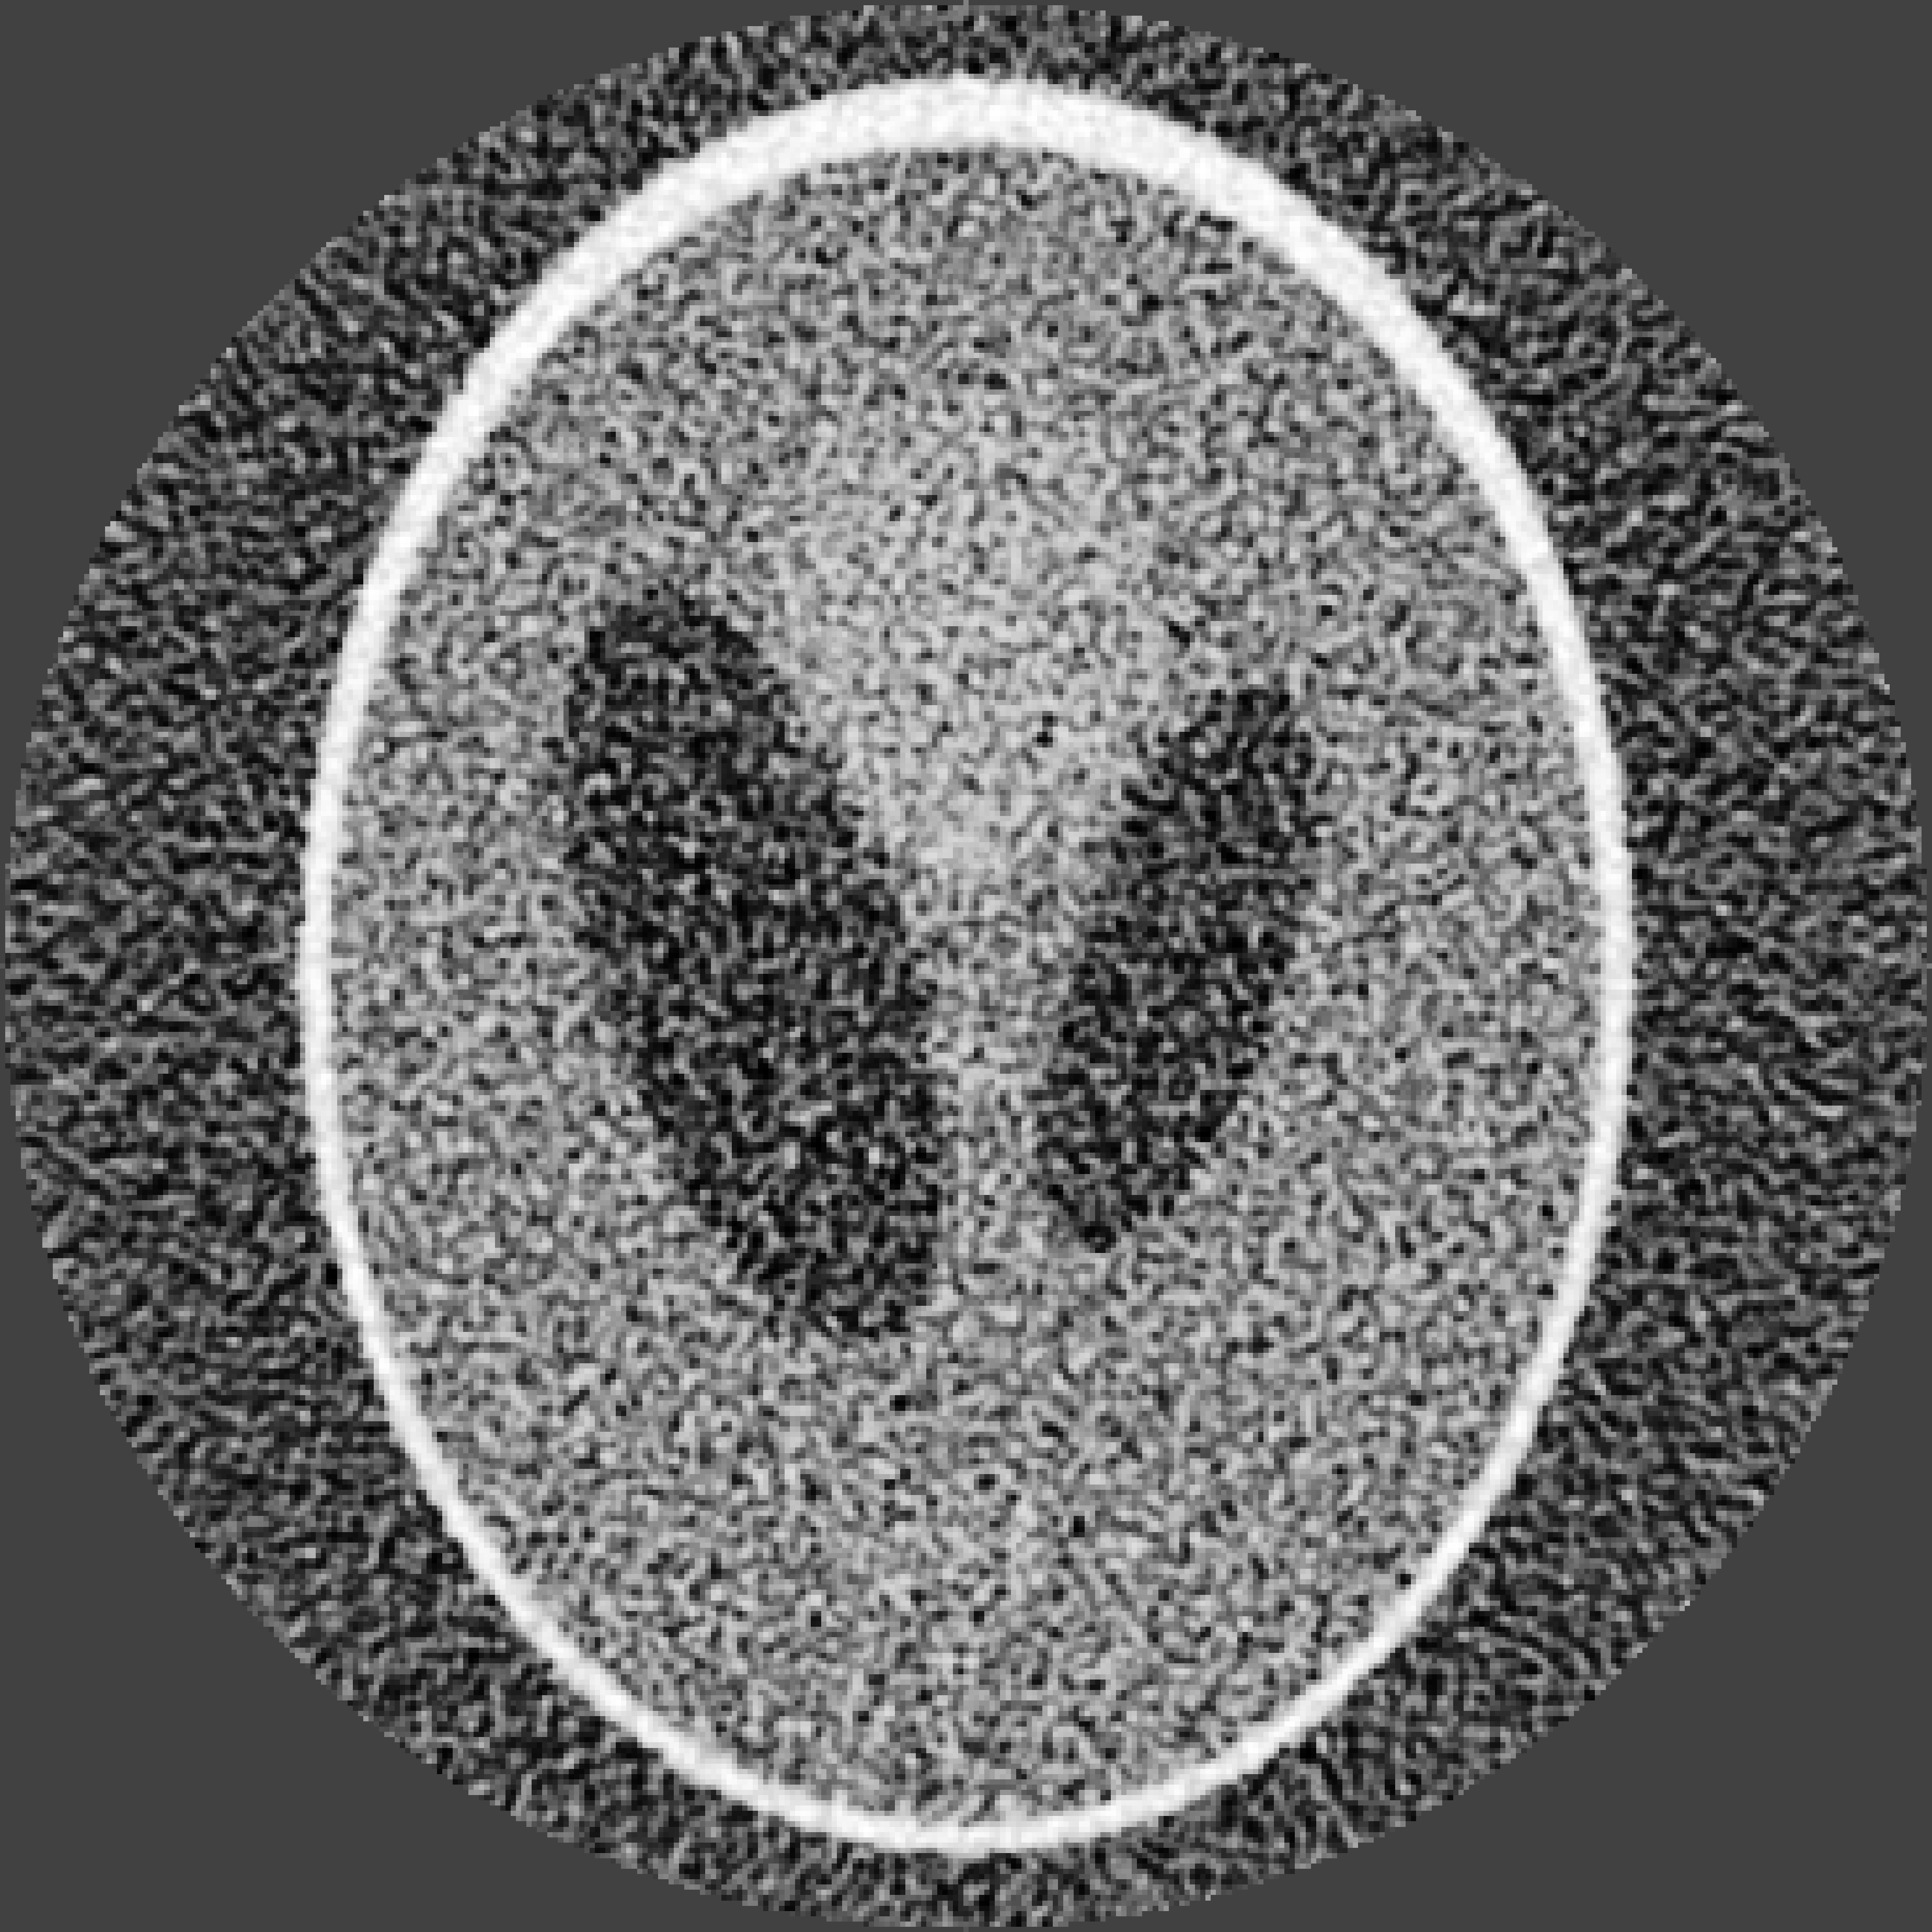
\includegraphics[width=\textwidth]{Figuras/reconstruction_hann_EQ.png}
            \caption{Filtro Hahn.}
            \label{fig:noise_hahn}
      \end{subfigure}
   \caption{Sinograma con ruido gaussiano (a). Reconstrucciones con filtro rampa (b), Shepp-Logan (c), coseno (d), Hamming (e) y Hahn (f). Todas las reconstrucciones fueron ecualizadas para ampliar el rango dinámico de la imagen.}
   \label{fig:noise_vs_filters}
\end{figure}

En la Fig. \ref{fig:noise_vs_filters} no se observa una gran diferencia entre los filtros, por lo tanto se calculó el error de reconstrucción para cada filtro a fin de calcular el efecto de los mismos en la reconstrucción. En la Fig. \ref{fig:error_filters_noise} se muestra el error de reconstrucción para cada filtro y en la Fig. \ref{fig:comp_filters} se muestra el efecto de cada filtro en el dominio de frecuencias. Se observa que para un dado filtro, cuanto menos pesa las altas frecuencias mejor reconstrucción produce.

\begin{figure}[H]
   \centering         
   \begin{subfigure}[h]{0.49\linewidth}
      \centering
      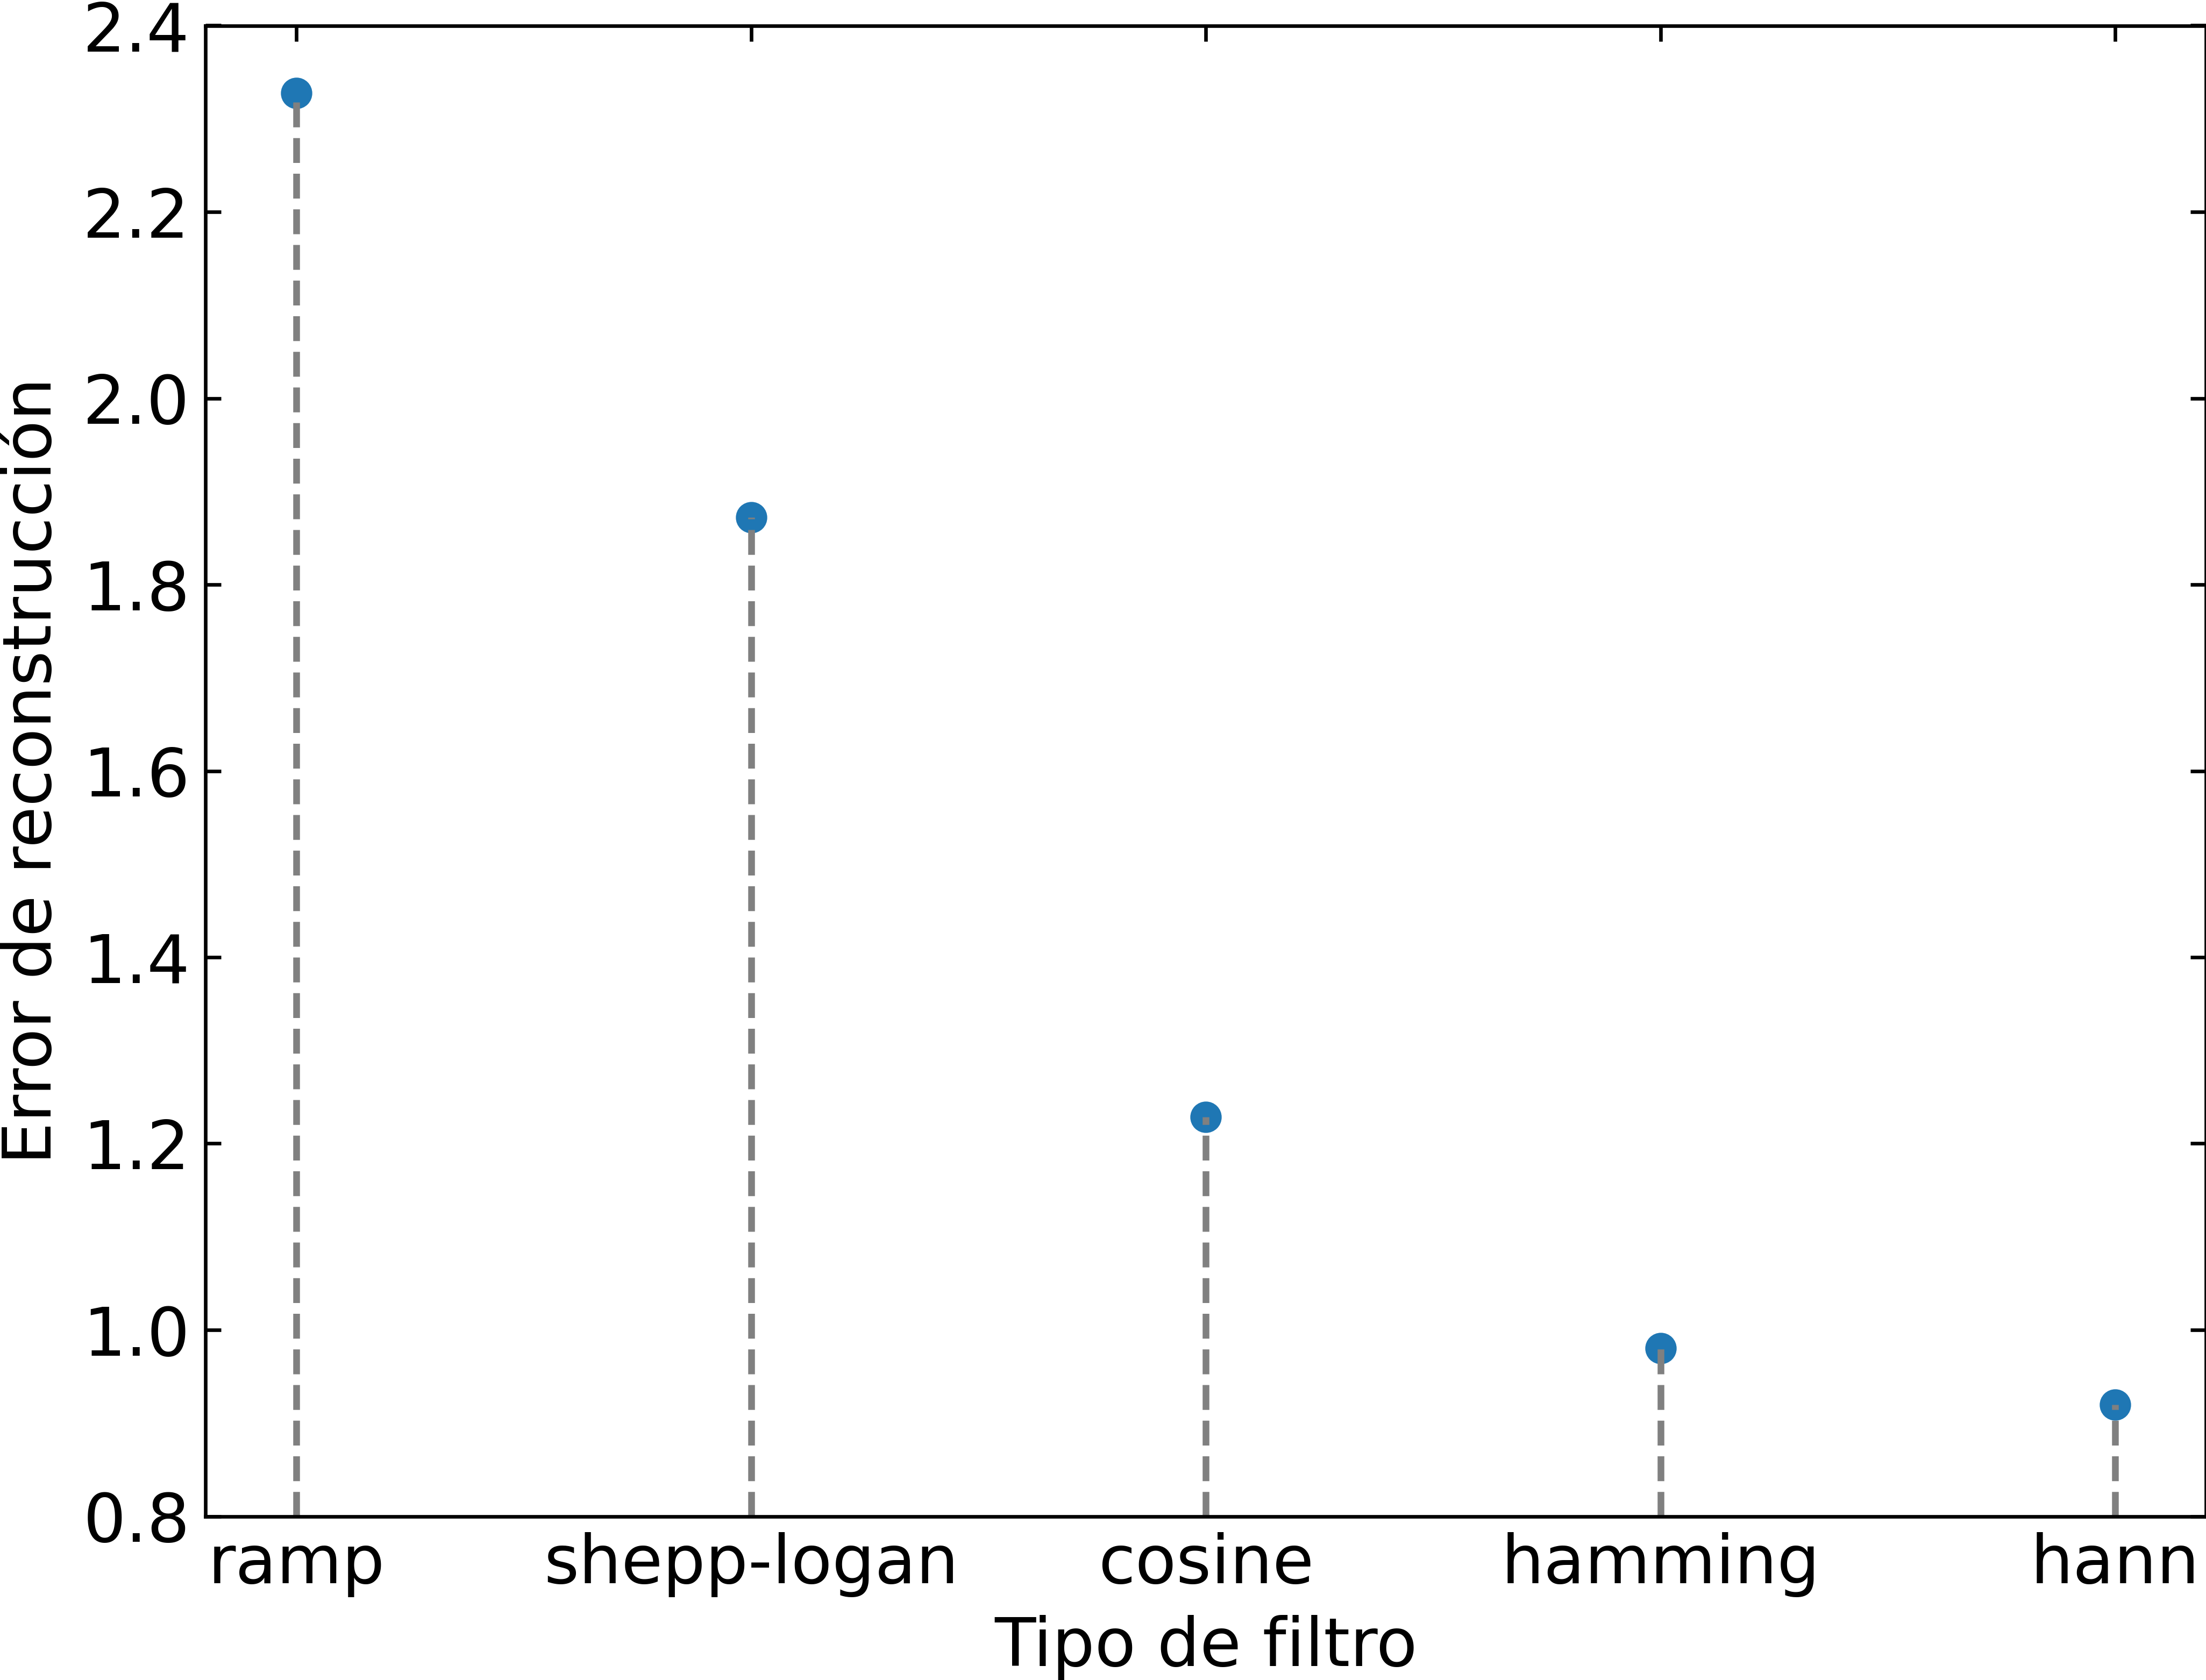
\includegraphics[width=\textwidth]{Figuras/error_vs_filters_noise.png}
      \caption{}
      \label{fig:error_filters_noise}
   \end{subfigure}
   \begin{subfigure}[h]{0.49\linewidth}
      \centering
      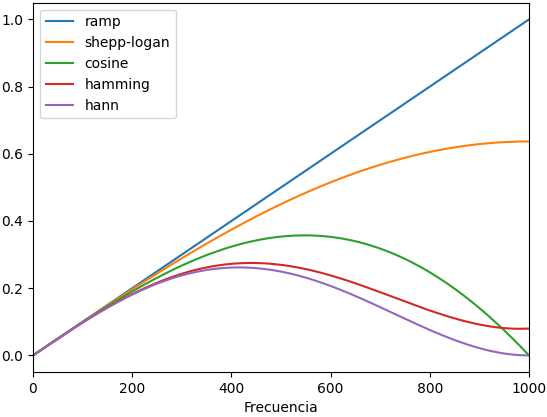
\includegraphics[width=\textwidth]{Figuras/comp_filters.png}
      \caption{}
      \label{fig:comp_filters}
   \end{subfigure}
   \caption{(a) Error de reconstrucción para cada filtro aplicado sobre el sinograma con ruido. (b) Efecto de cada filtro en el dominio de frecuencias.}
   \label{fig:filters_noise}
\end{figure}

\section{Proyecciones paralelas de un círculo}

Utilizando la libreria $\verb|OpenCV|$ de Python se creó una imagen de $100\times100$ negra con un círculo blanco de radio $3$ pixels centrado en el medio de la imagen como se muestra en la Fig. \ref{fig:sinograma_circulo}. Utilizando el programa provisto $\verb|radon-skimage.py|$ se generó un sinograma de esta imagen con 100 detectores y se varió el número de proyecciones en $8,16,32,64$. Además para cada caso, se utilizó retroproyección con filtro rampa y sin filtro. Los resultados se encuentran en la Fig. \ref{fig:retroproyeccion_circulo}.

\begin{figure}[H]
   \centering
         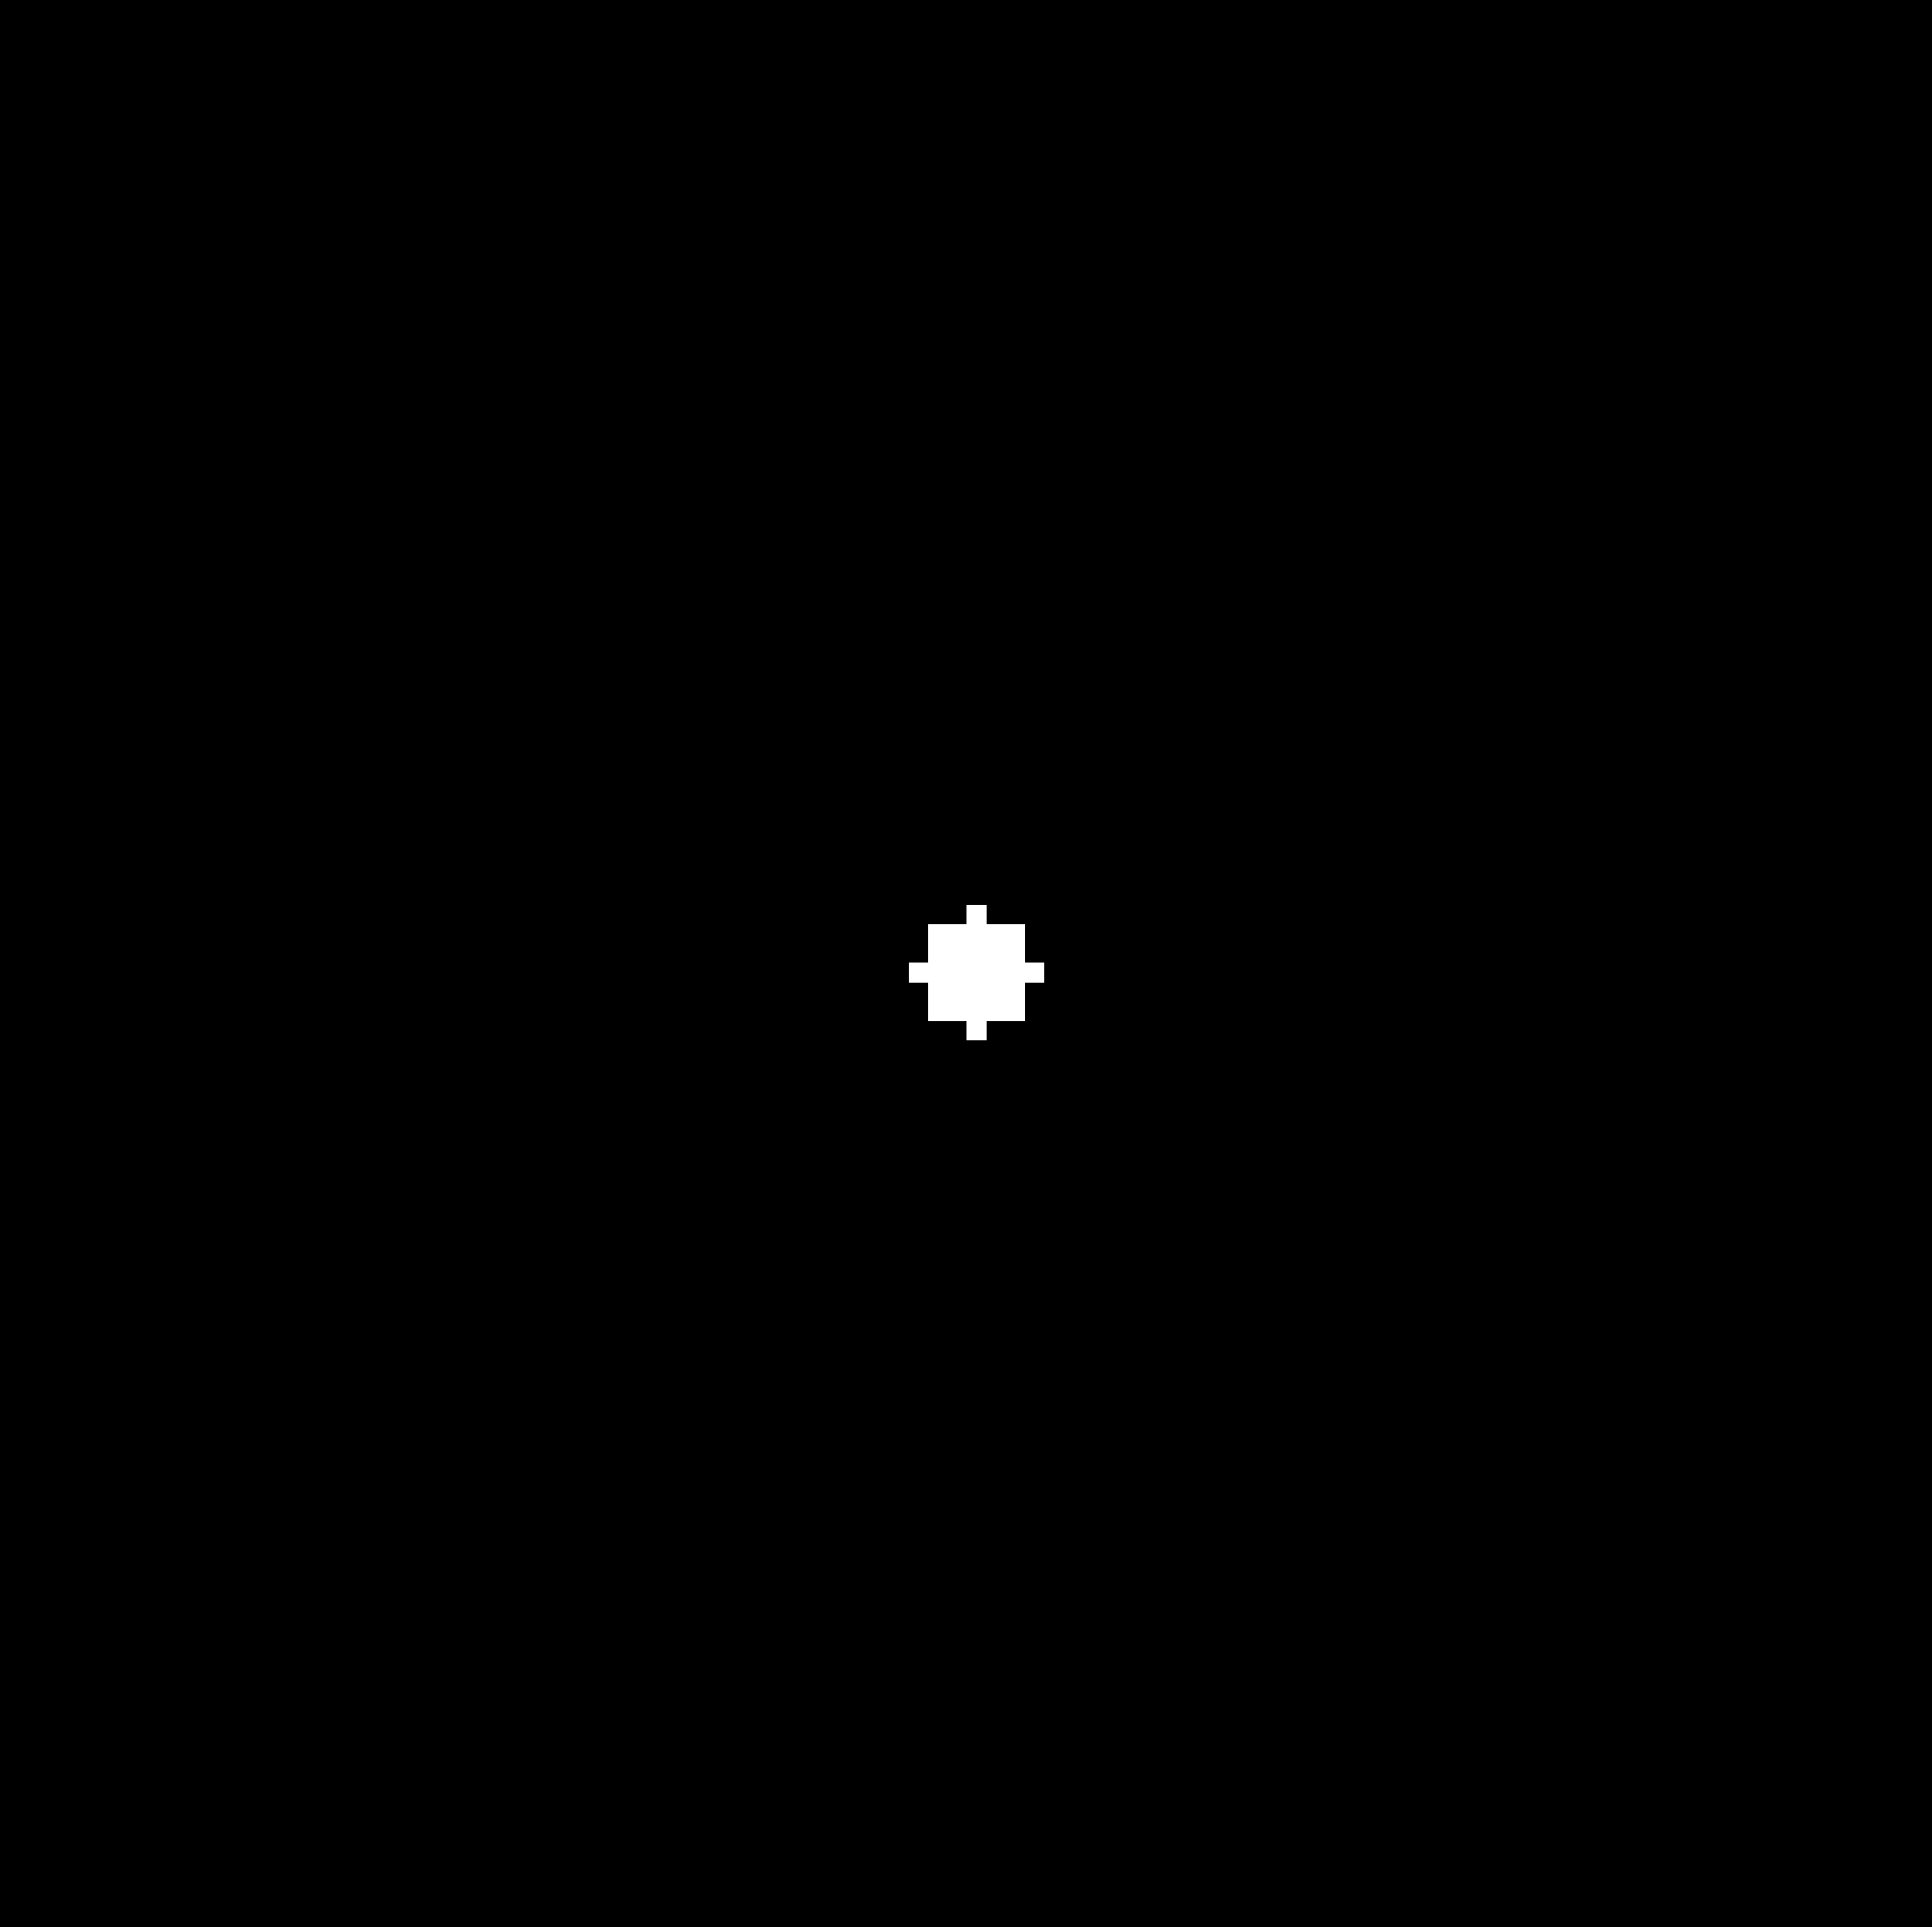
\includegraphics[width=0.3\textwidth]{Figuras/sinograma_circulo.png}
   \caption{(a) Imagen del círculo de 3 pixeles de radio. (b) Sinograma generado del círculo. }
   \label{fig:sinograma_circulo}
\end{figure}

En primer lugar, se nota que al aumentar el número de proyecciones disminuye notablemente el número de artefactos radiales en la reconstrucción de la imagen original. En cuanto a la aplicación del filtro rampa, se observa que el filtro reduce notablemente, o elimina el halo en el círculo, el cual si se observa para la retroproyección sin filtro. No obstante, para pocas proyecciones, el filtrado con filtro rampa amplifica la presencia de los artefactos radiales ya que los mismos se observan más definidos que en el caso sin rampa.

\begin{figure}[H]
   \centering
       \begin{subfigure}[h]{0.24\textwidth}
           \centering
           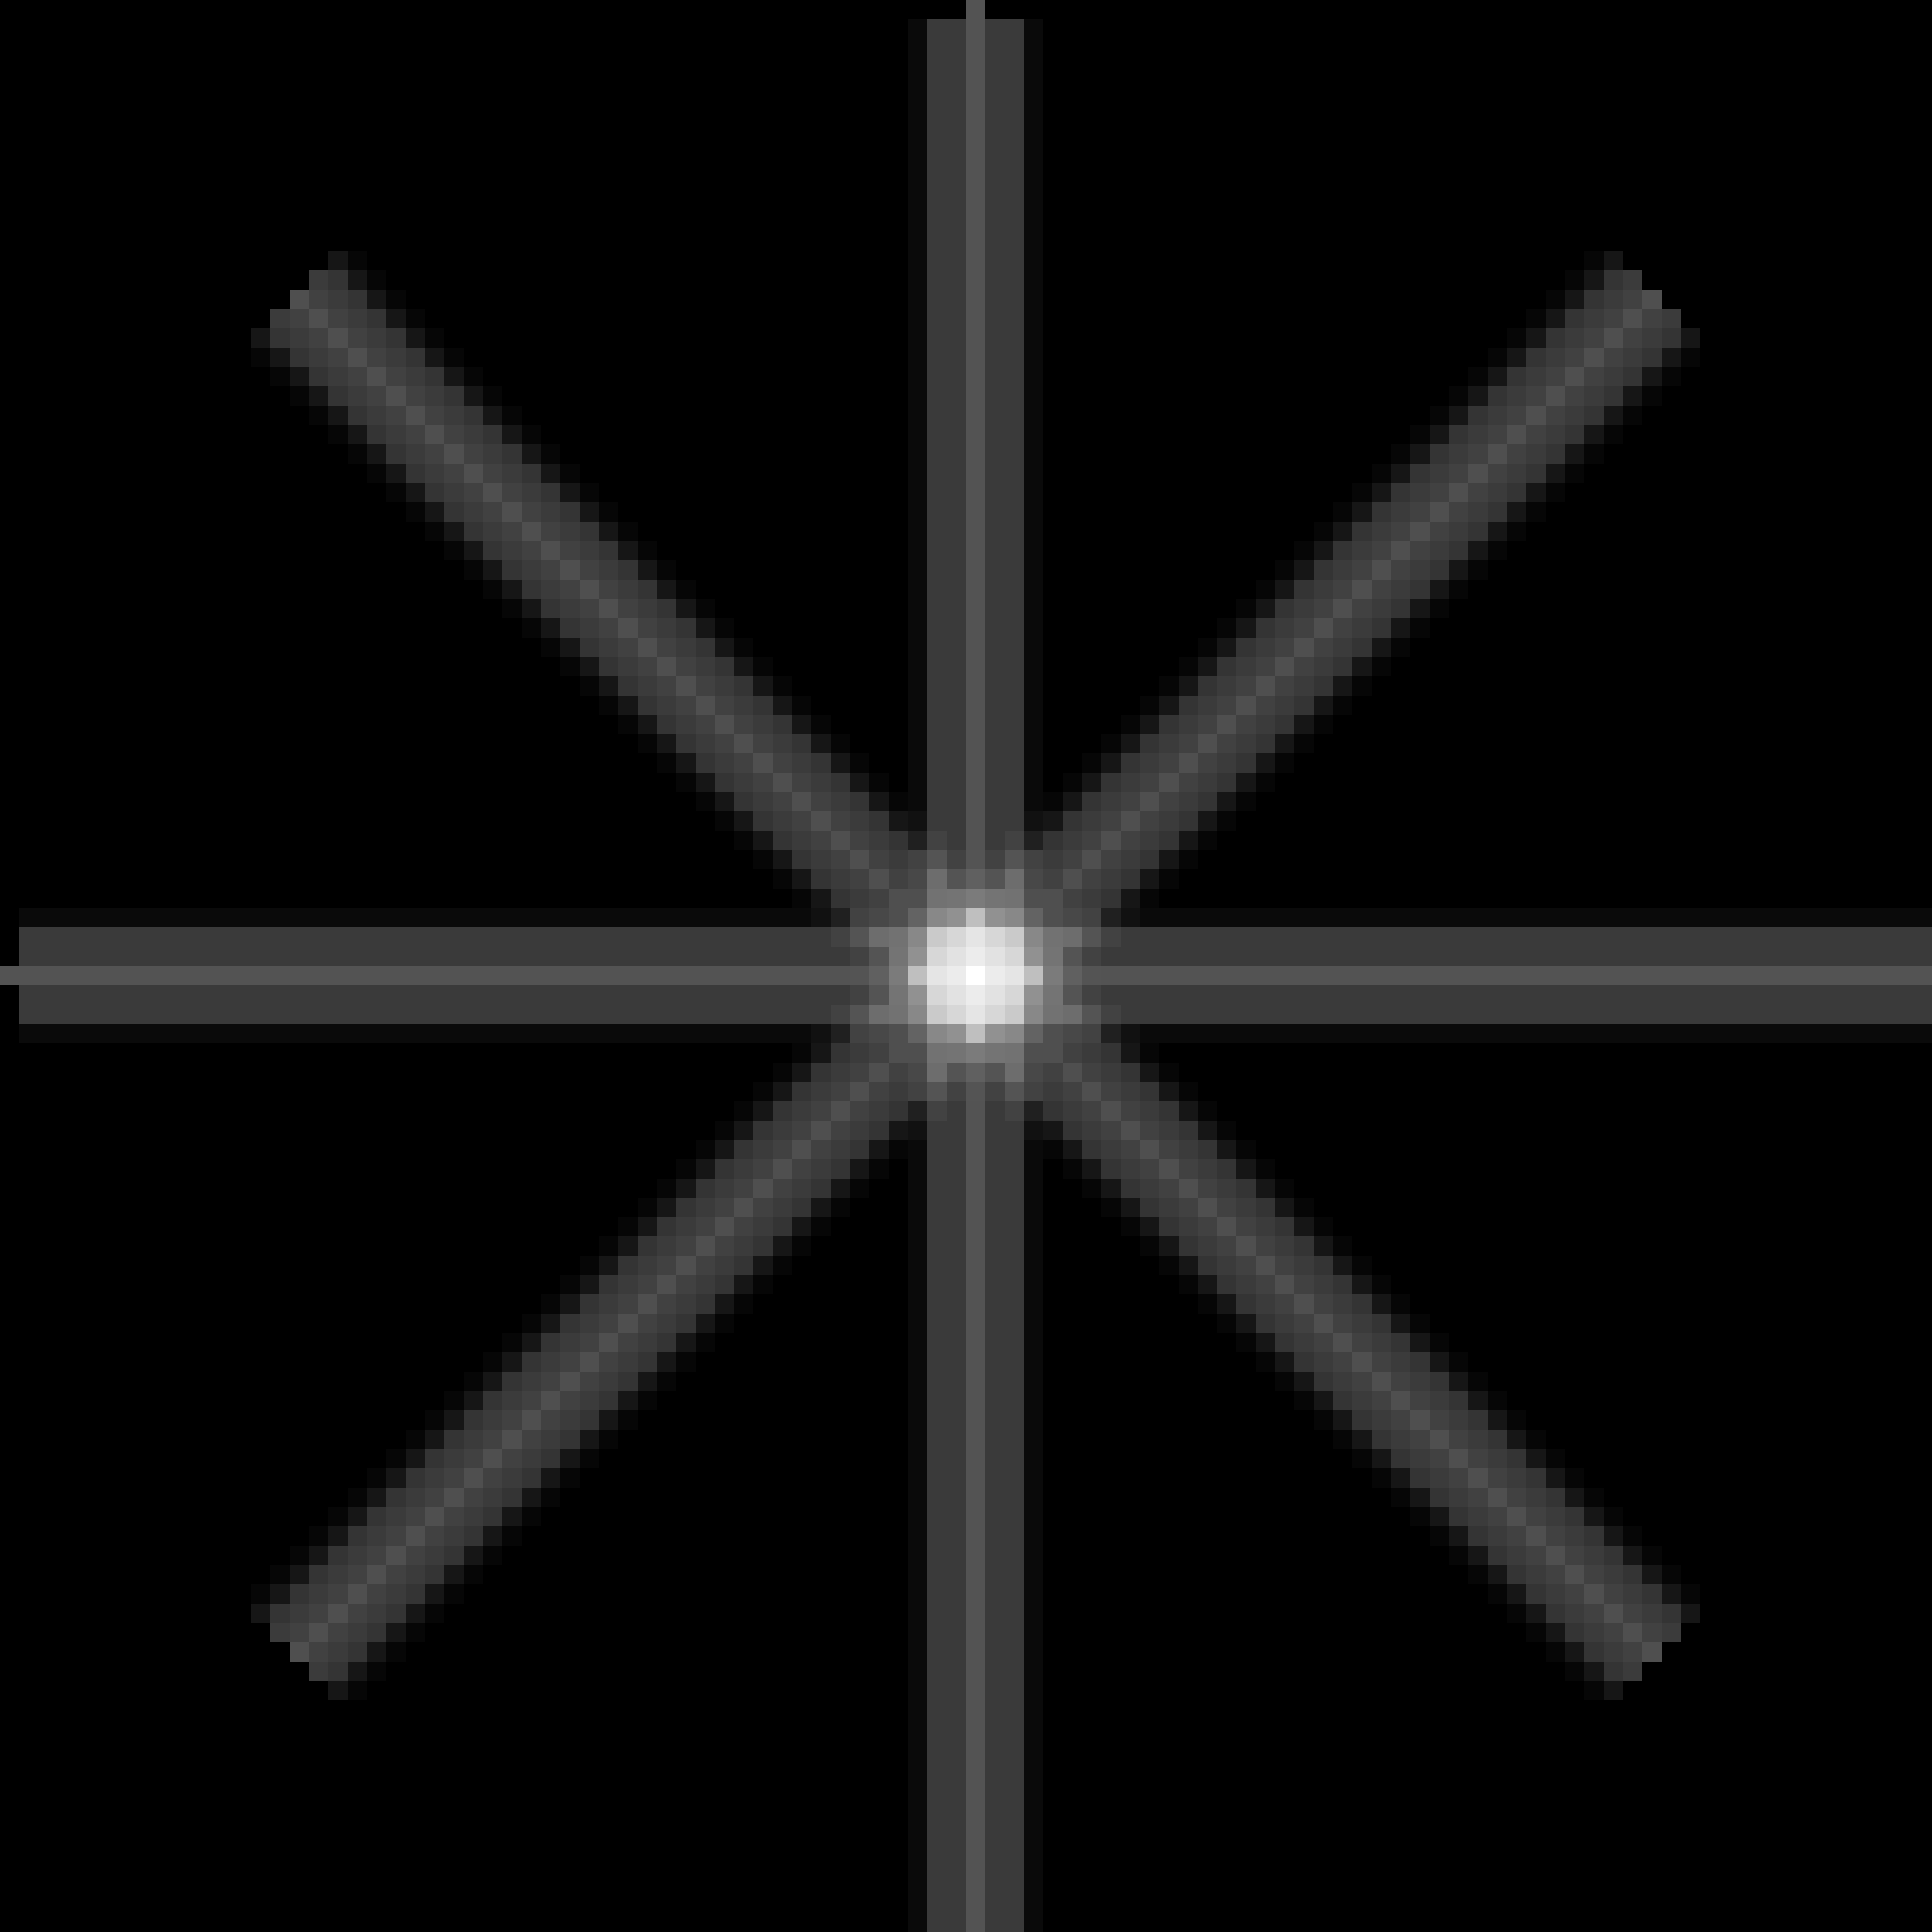
\includegraphics[width=\textwidth]{Figuras/retroproyeccion_p=8_filter=none.png} 
       \end{subfigure}
       \begin{subfigure}[h]{0.24\textwidth}
           \centering
           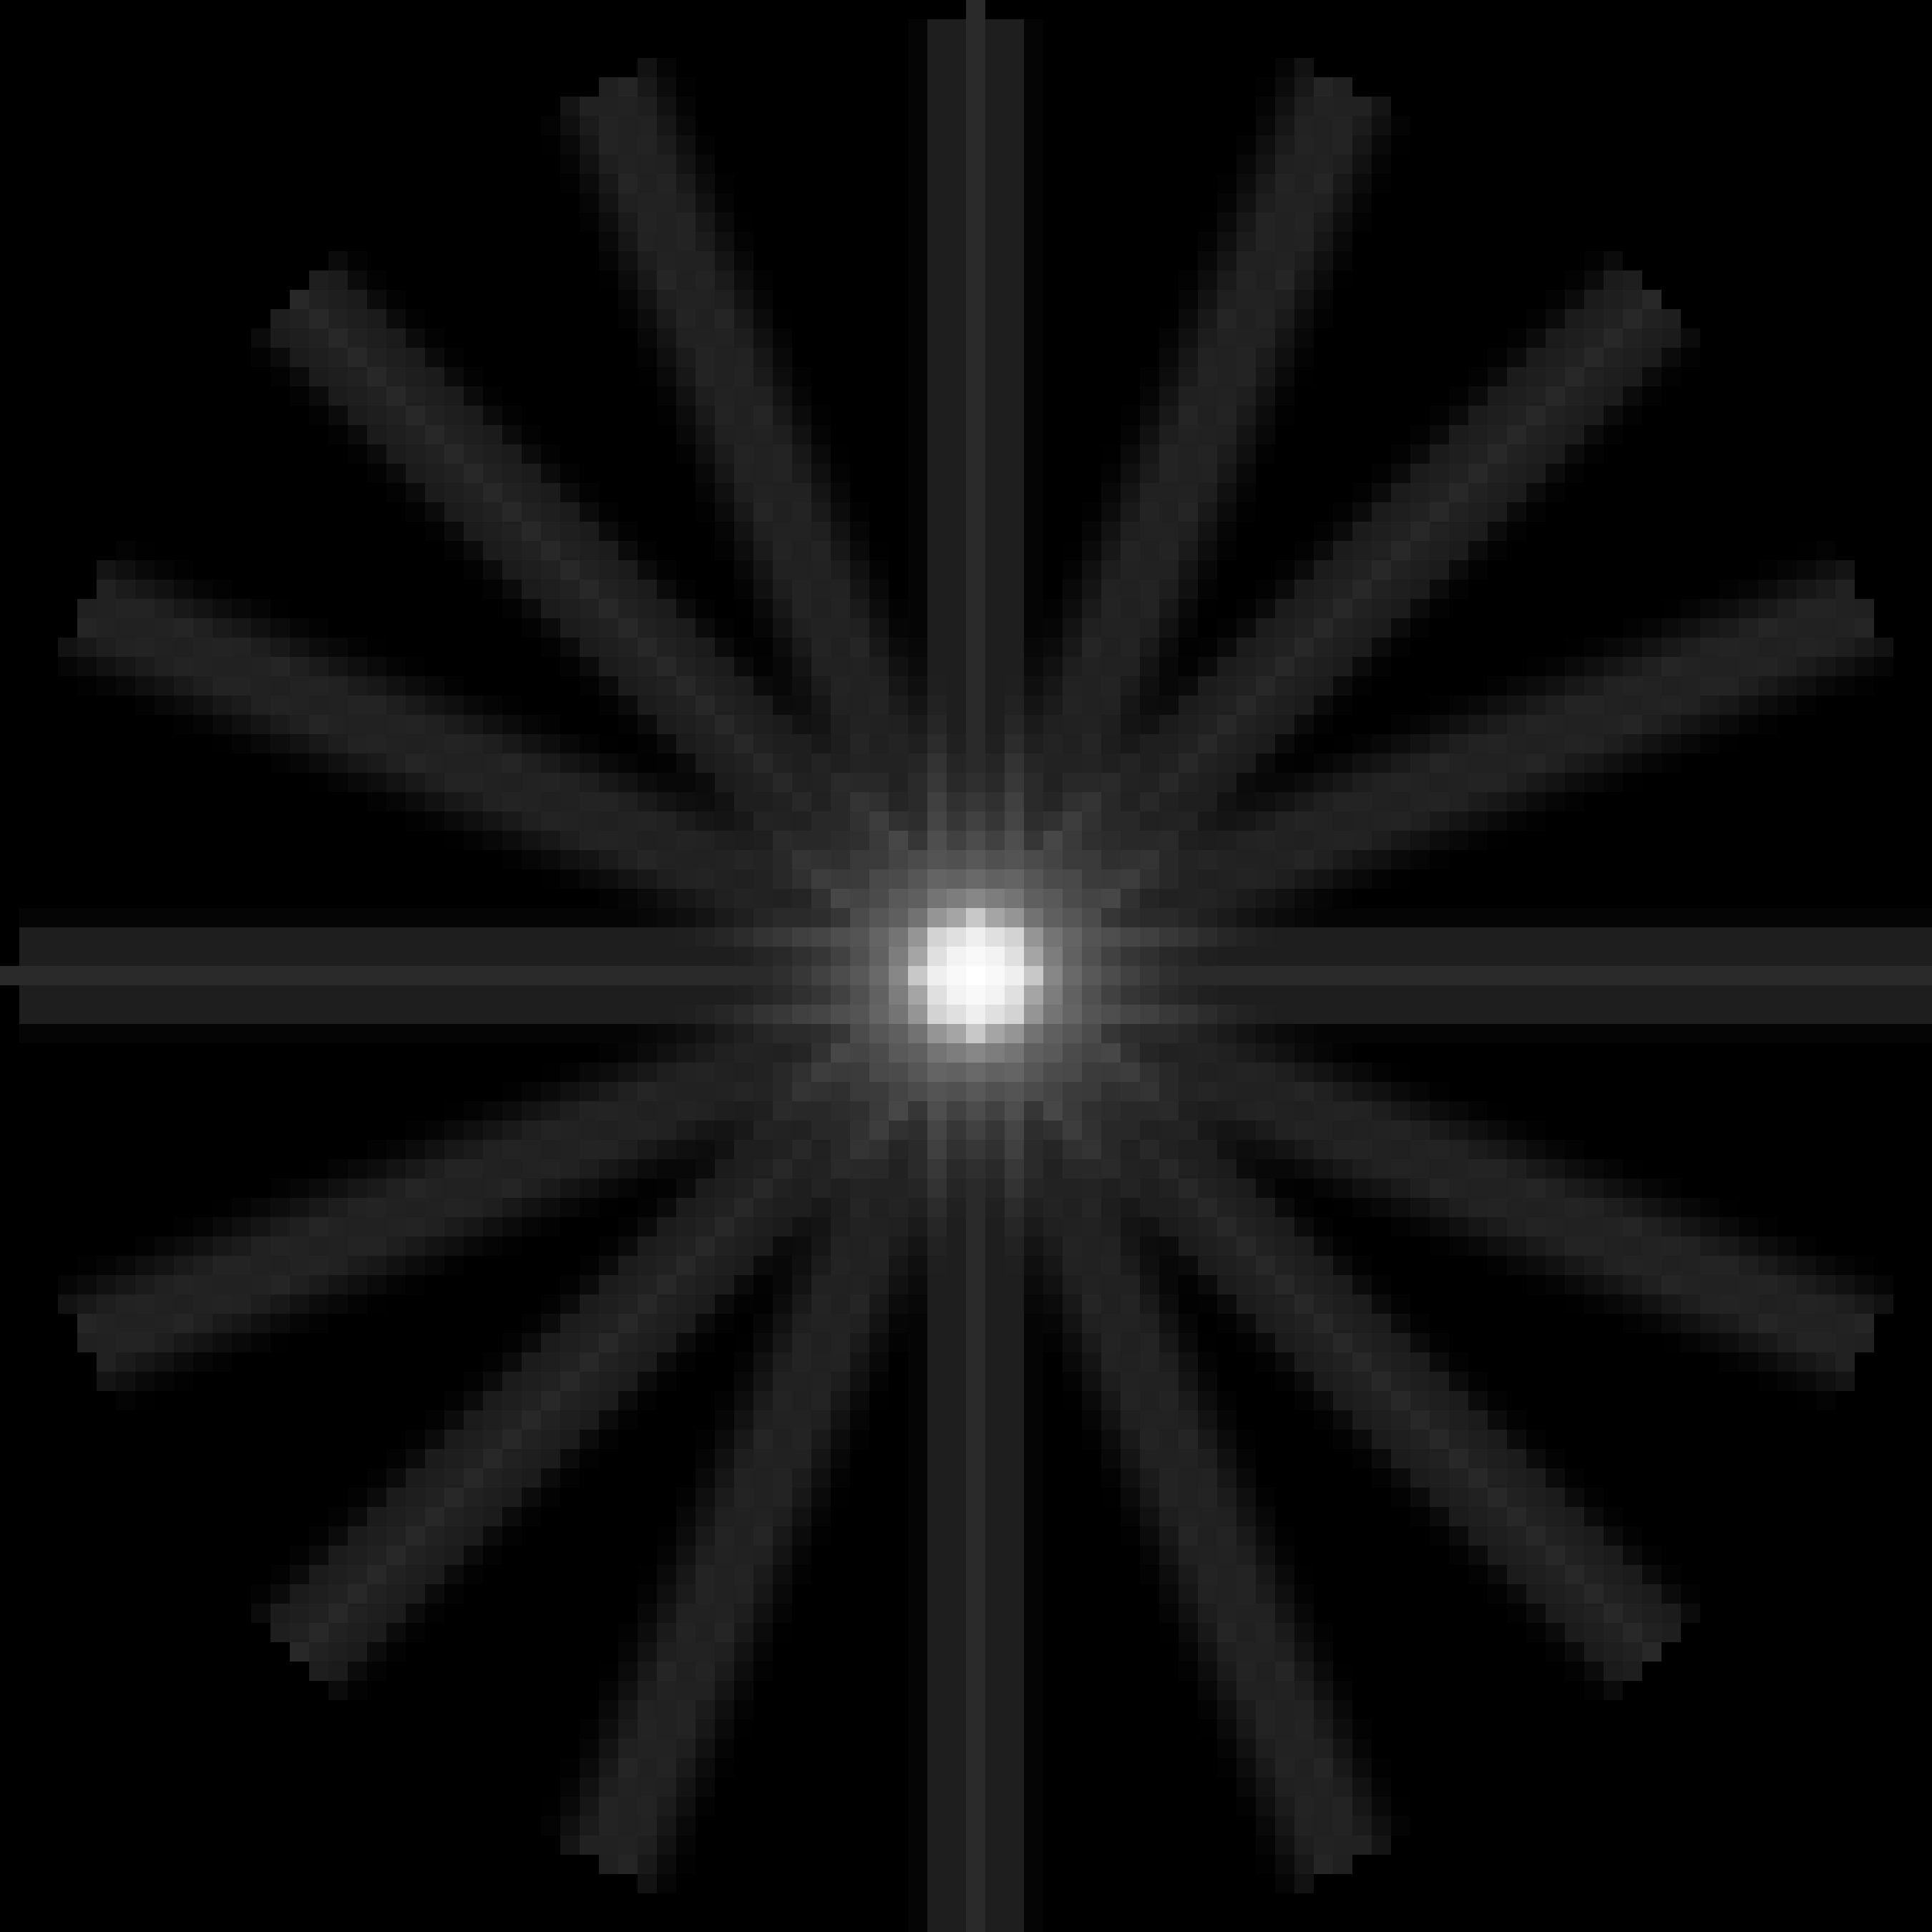
\includegraphics[width=\textwidth]{Figuras/retroproyeccion_p=16_filter=none.png}
       \end{subfigure}
       \begin{subfigure}[h]{0.24\textwidth}
           \centering
           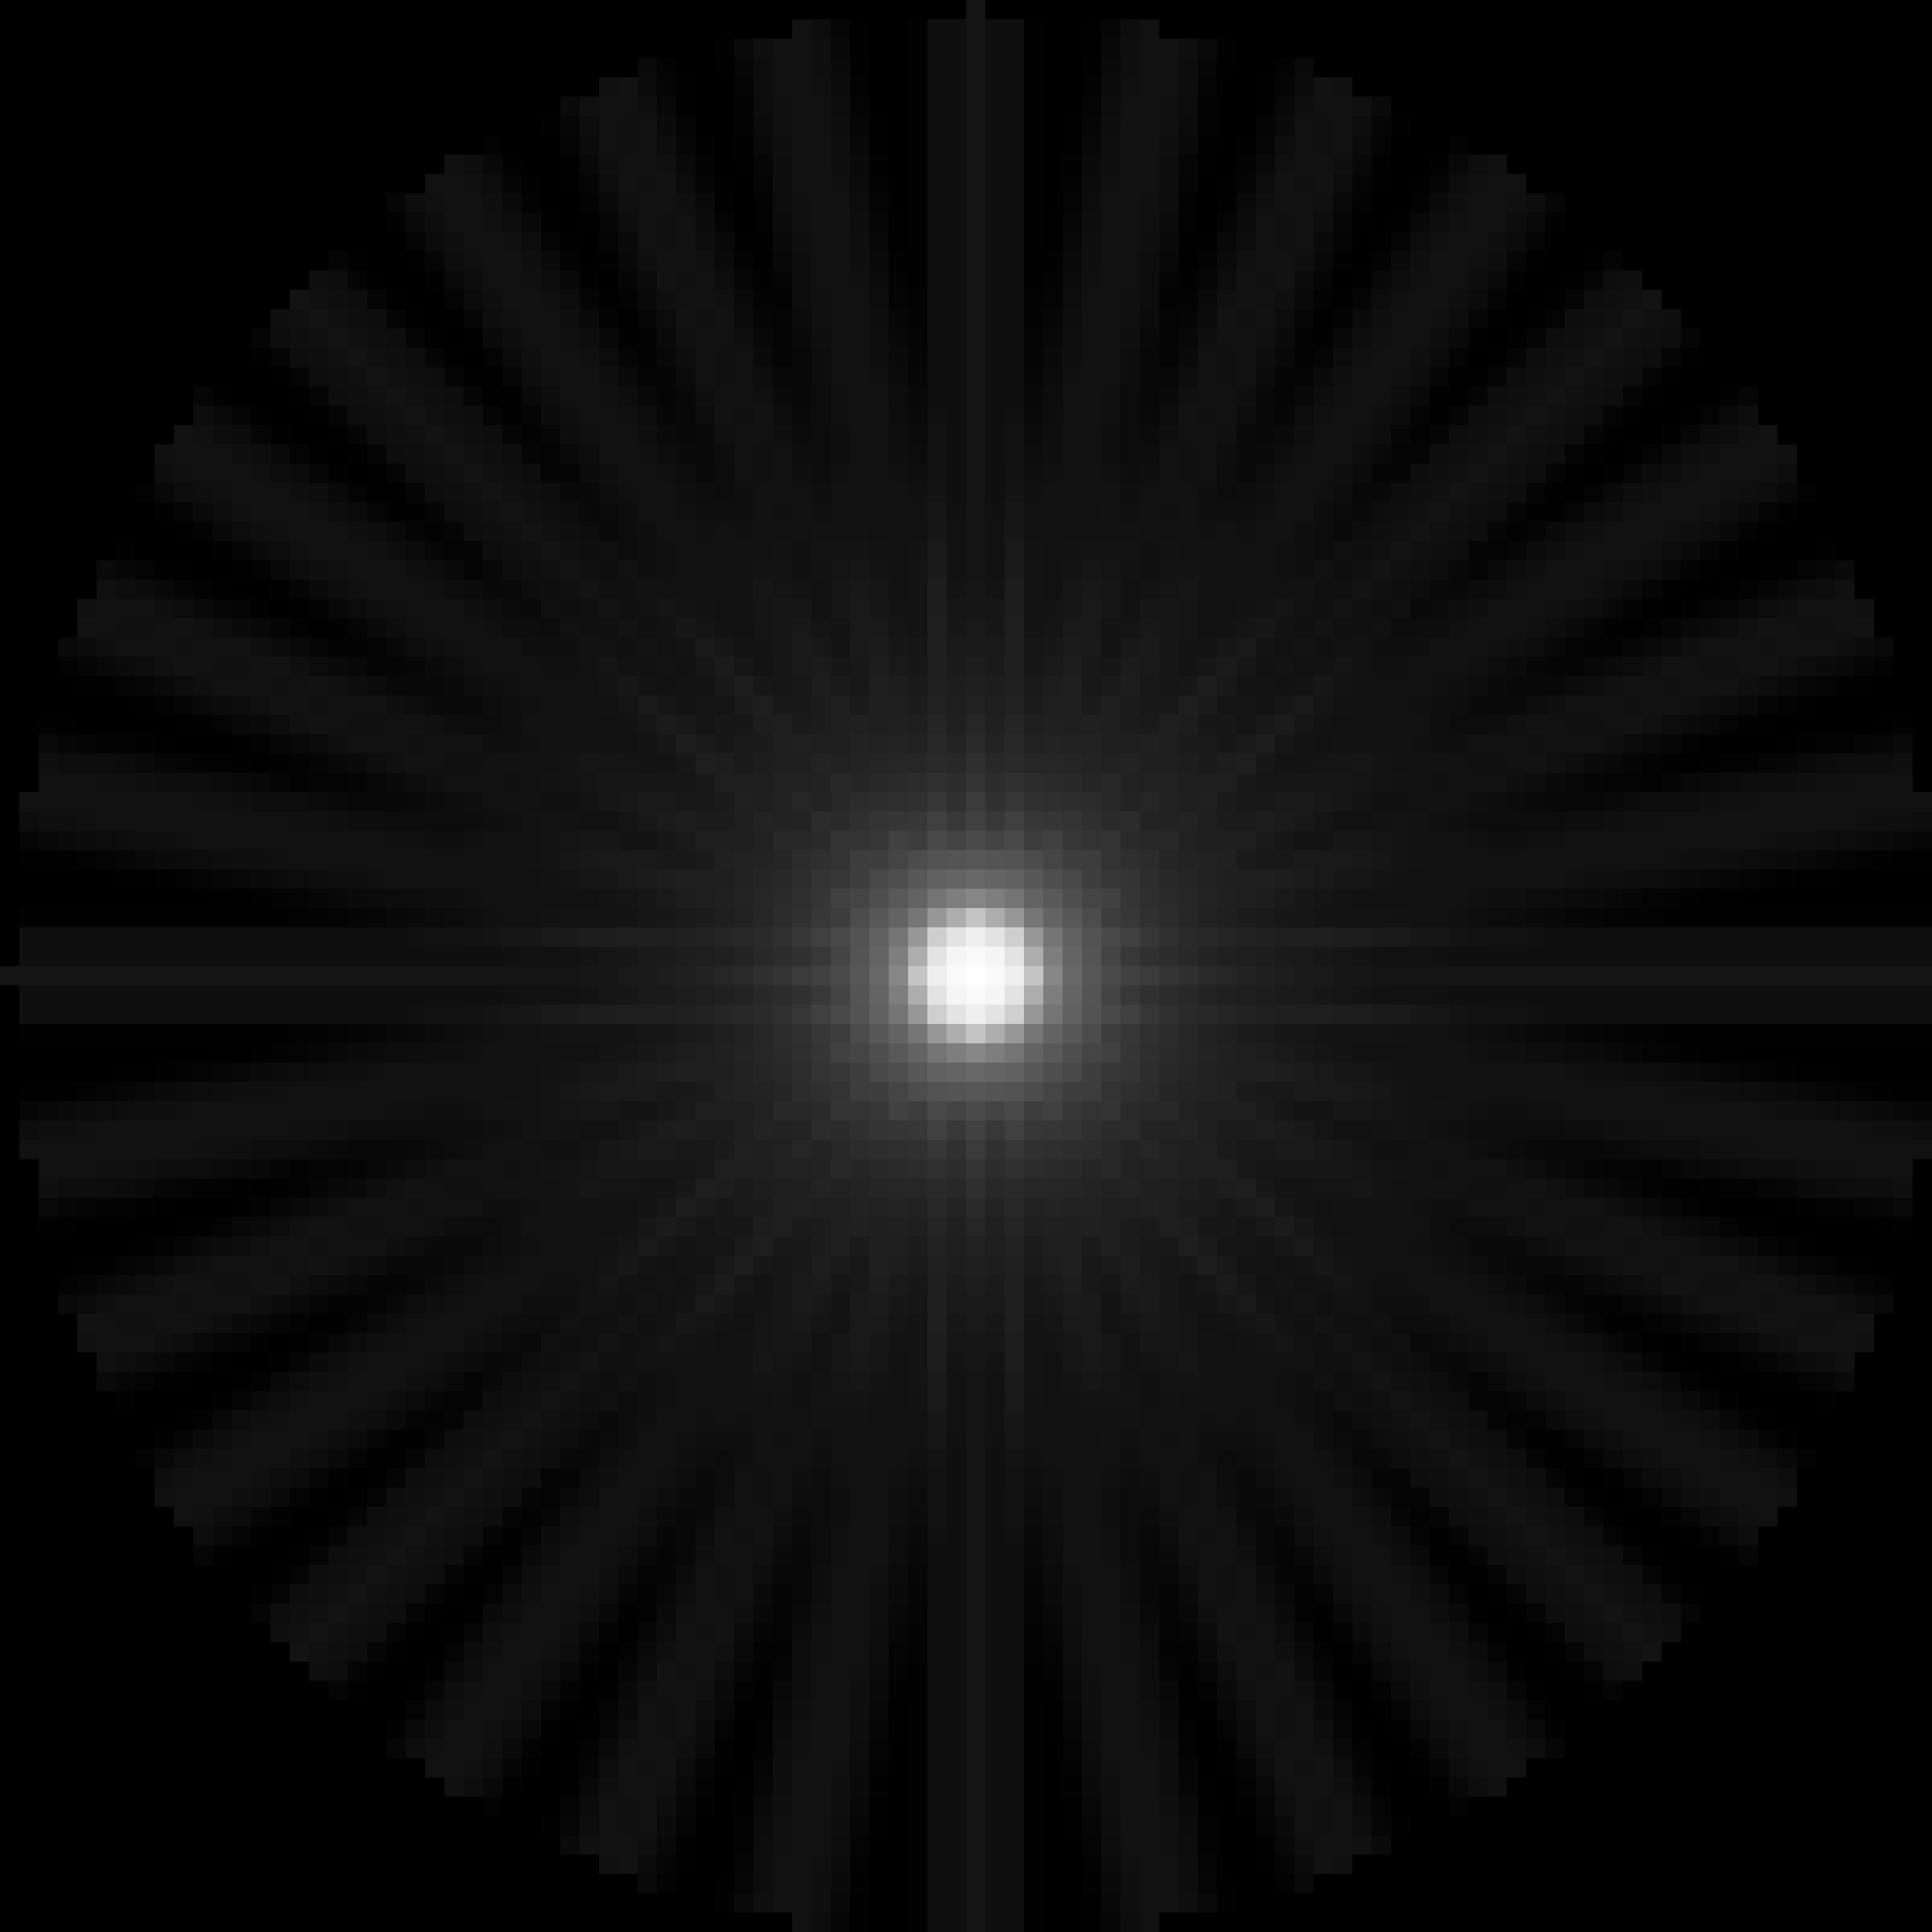
\includegraphics[width=\textwidth]{Figuras/retroproyeccion_p=32_filter=none.png}
       \end{subfigure}
       \begin{subfigure}[h]{0.24\textwidth}
           \centering
           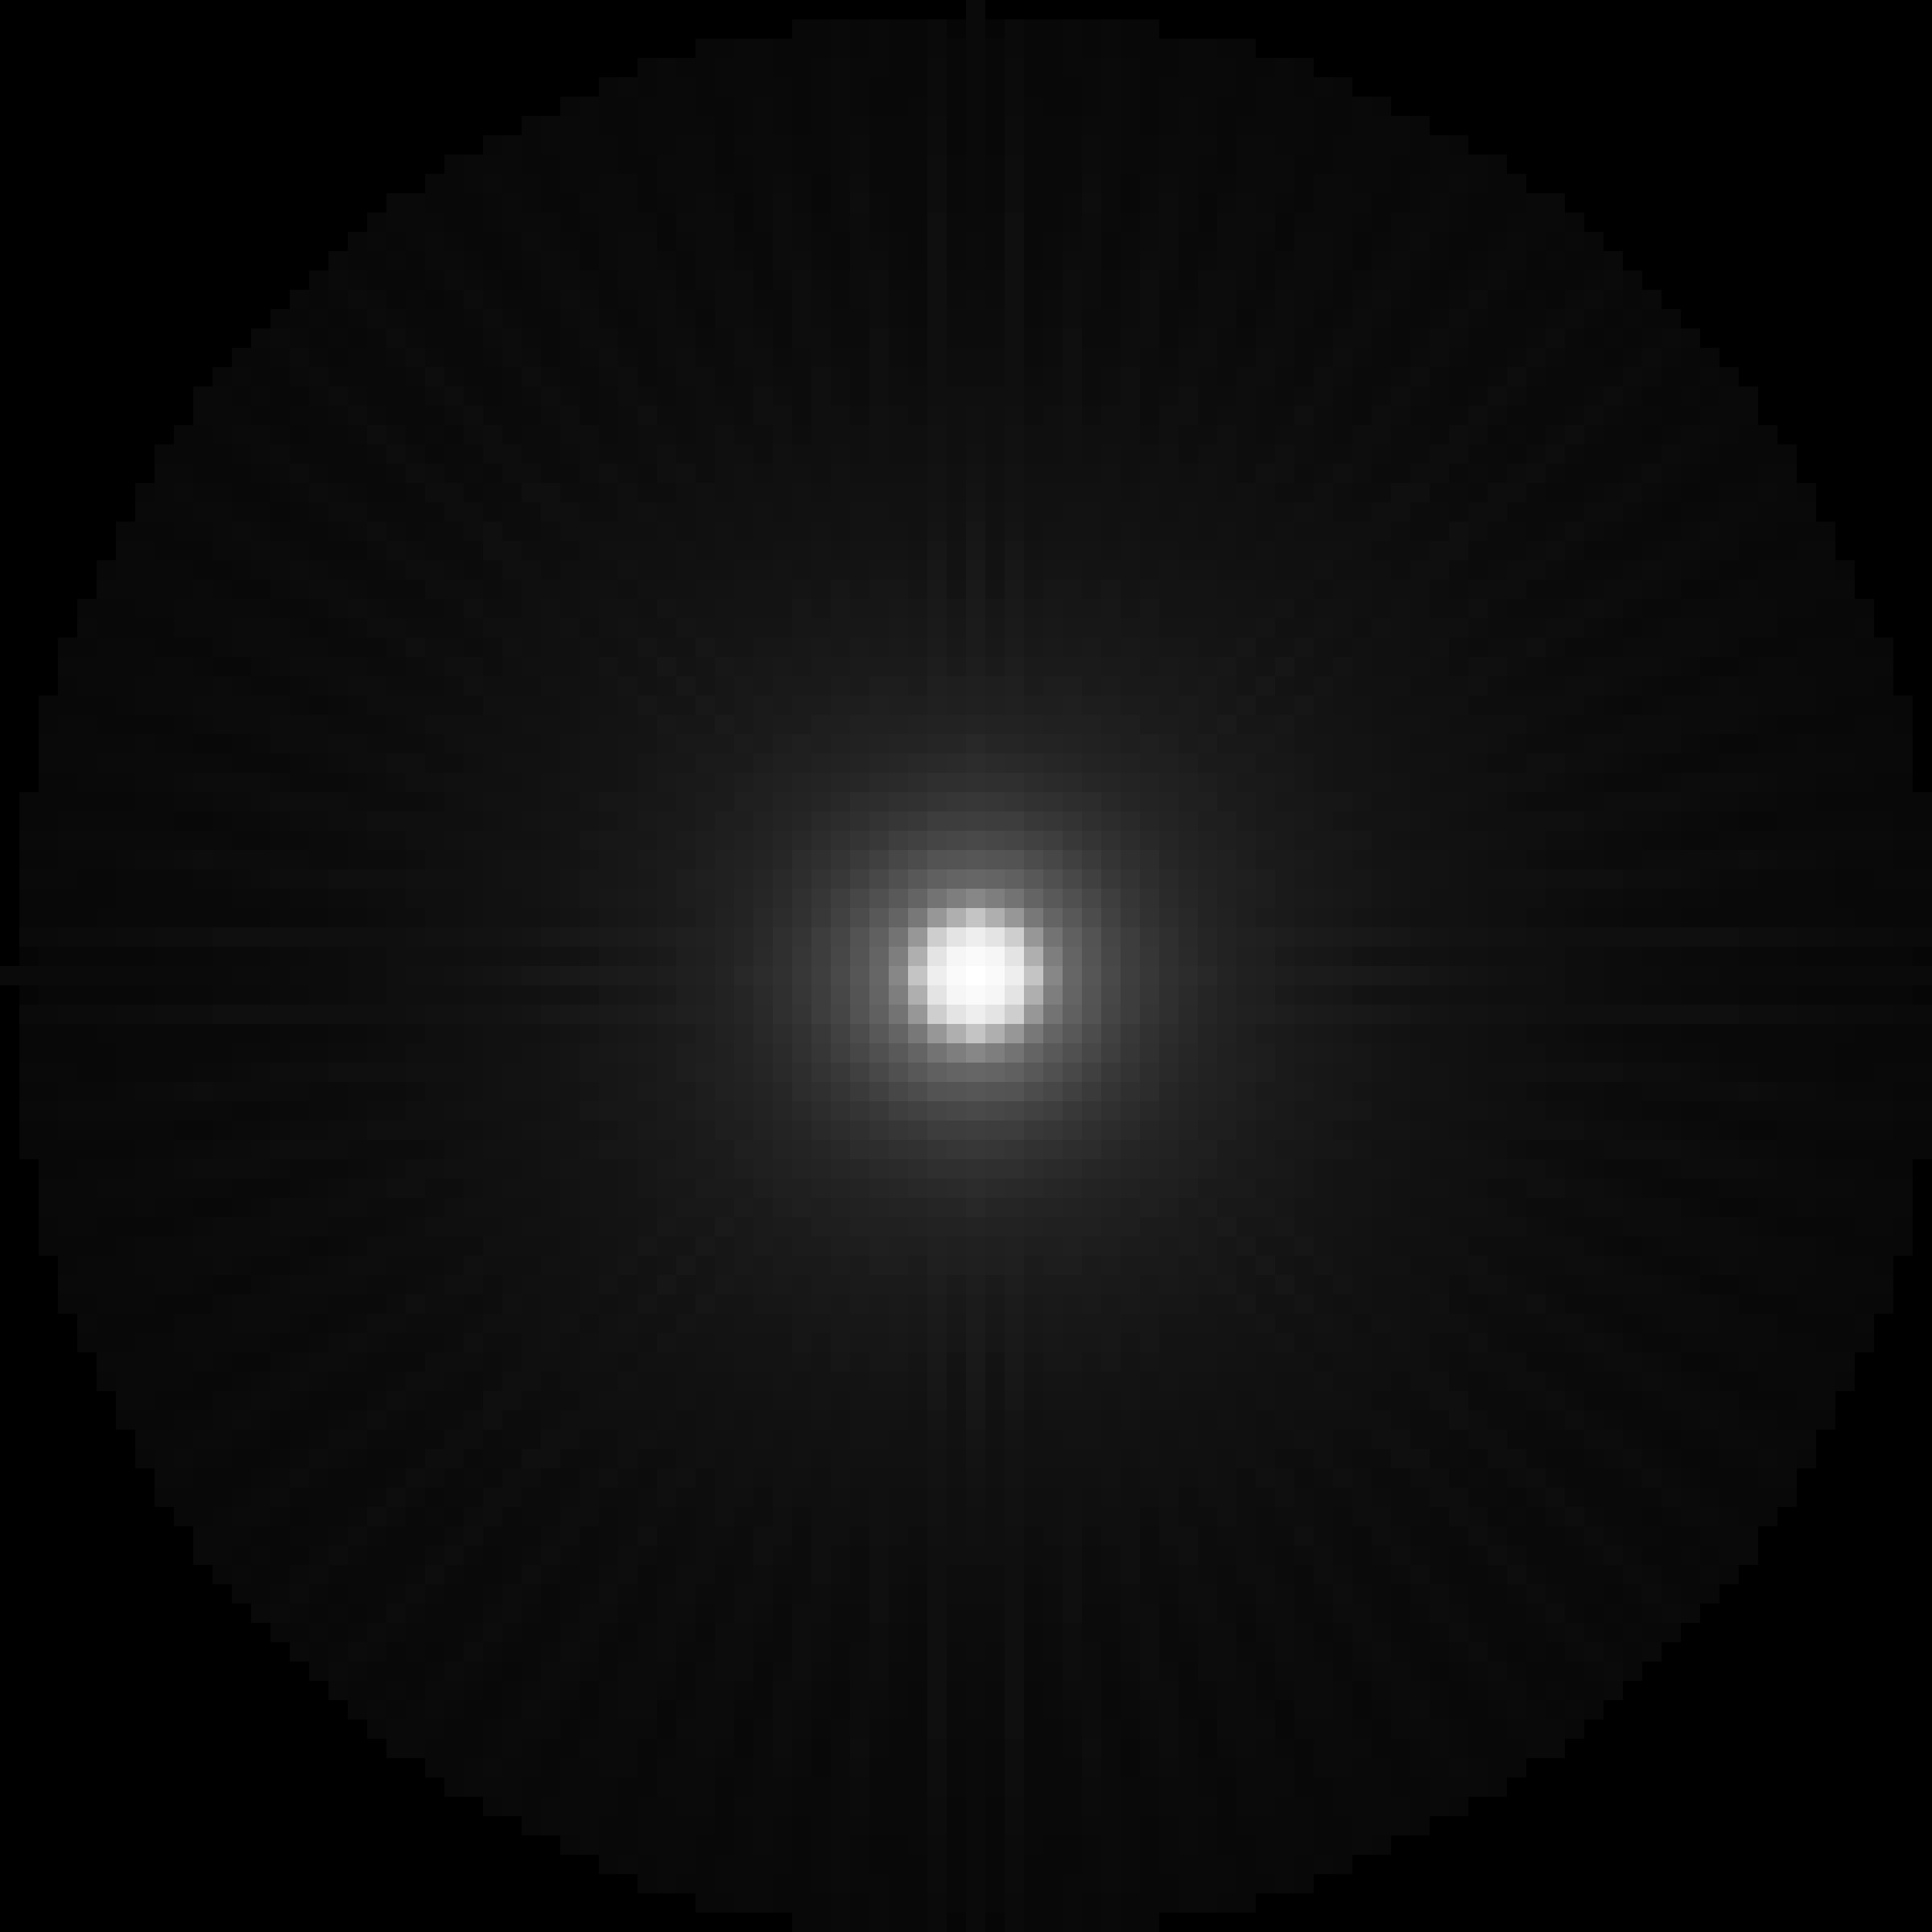
\includegraphics[width=\textwidth]{Figuras/retroproyeccion_p=64_filter=none.png}
       \end{subfigure}
        \begin{subfigure}[h]{0.24\textwidth}
           \centering
           
\includegraphics[width=\textwidth]{Figuras/retroproyeccion_p=8_filter=ramp.png}
           \caption{8 proyecciones.} 
        \end{subfigure}
        \begin{subfigure}[h]{0.24\textwidth}
           \centering
           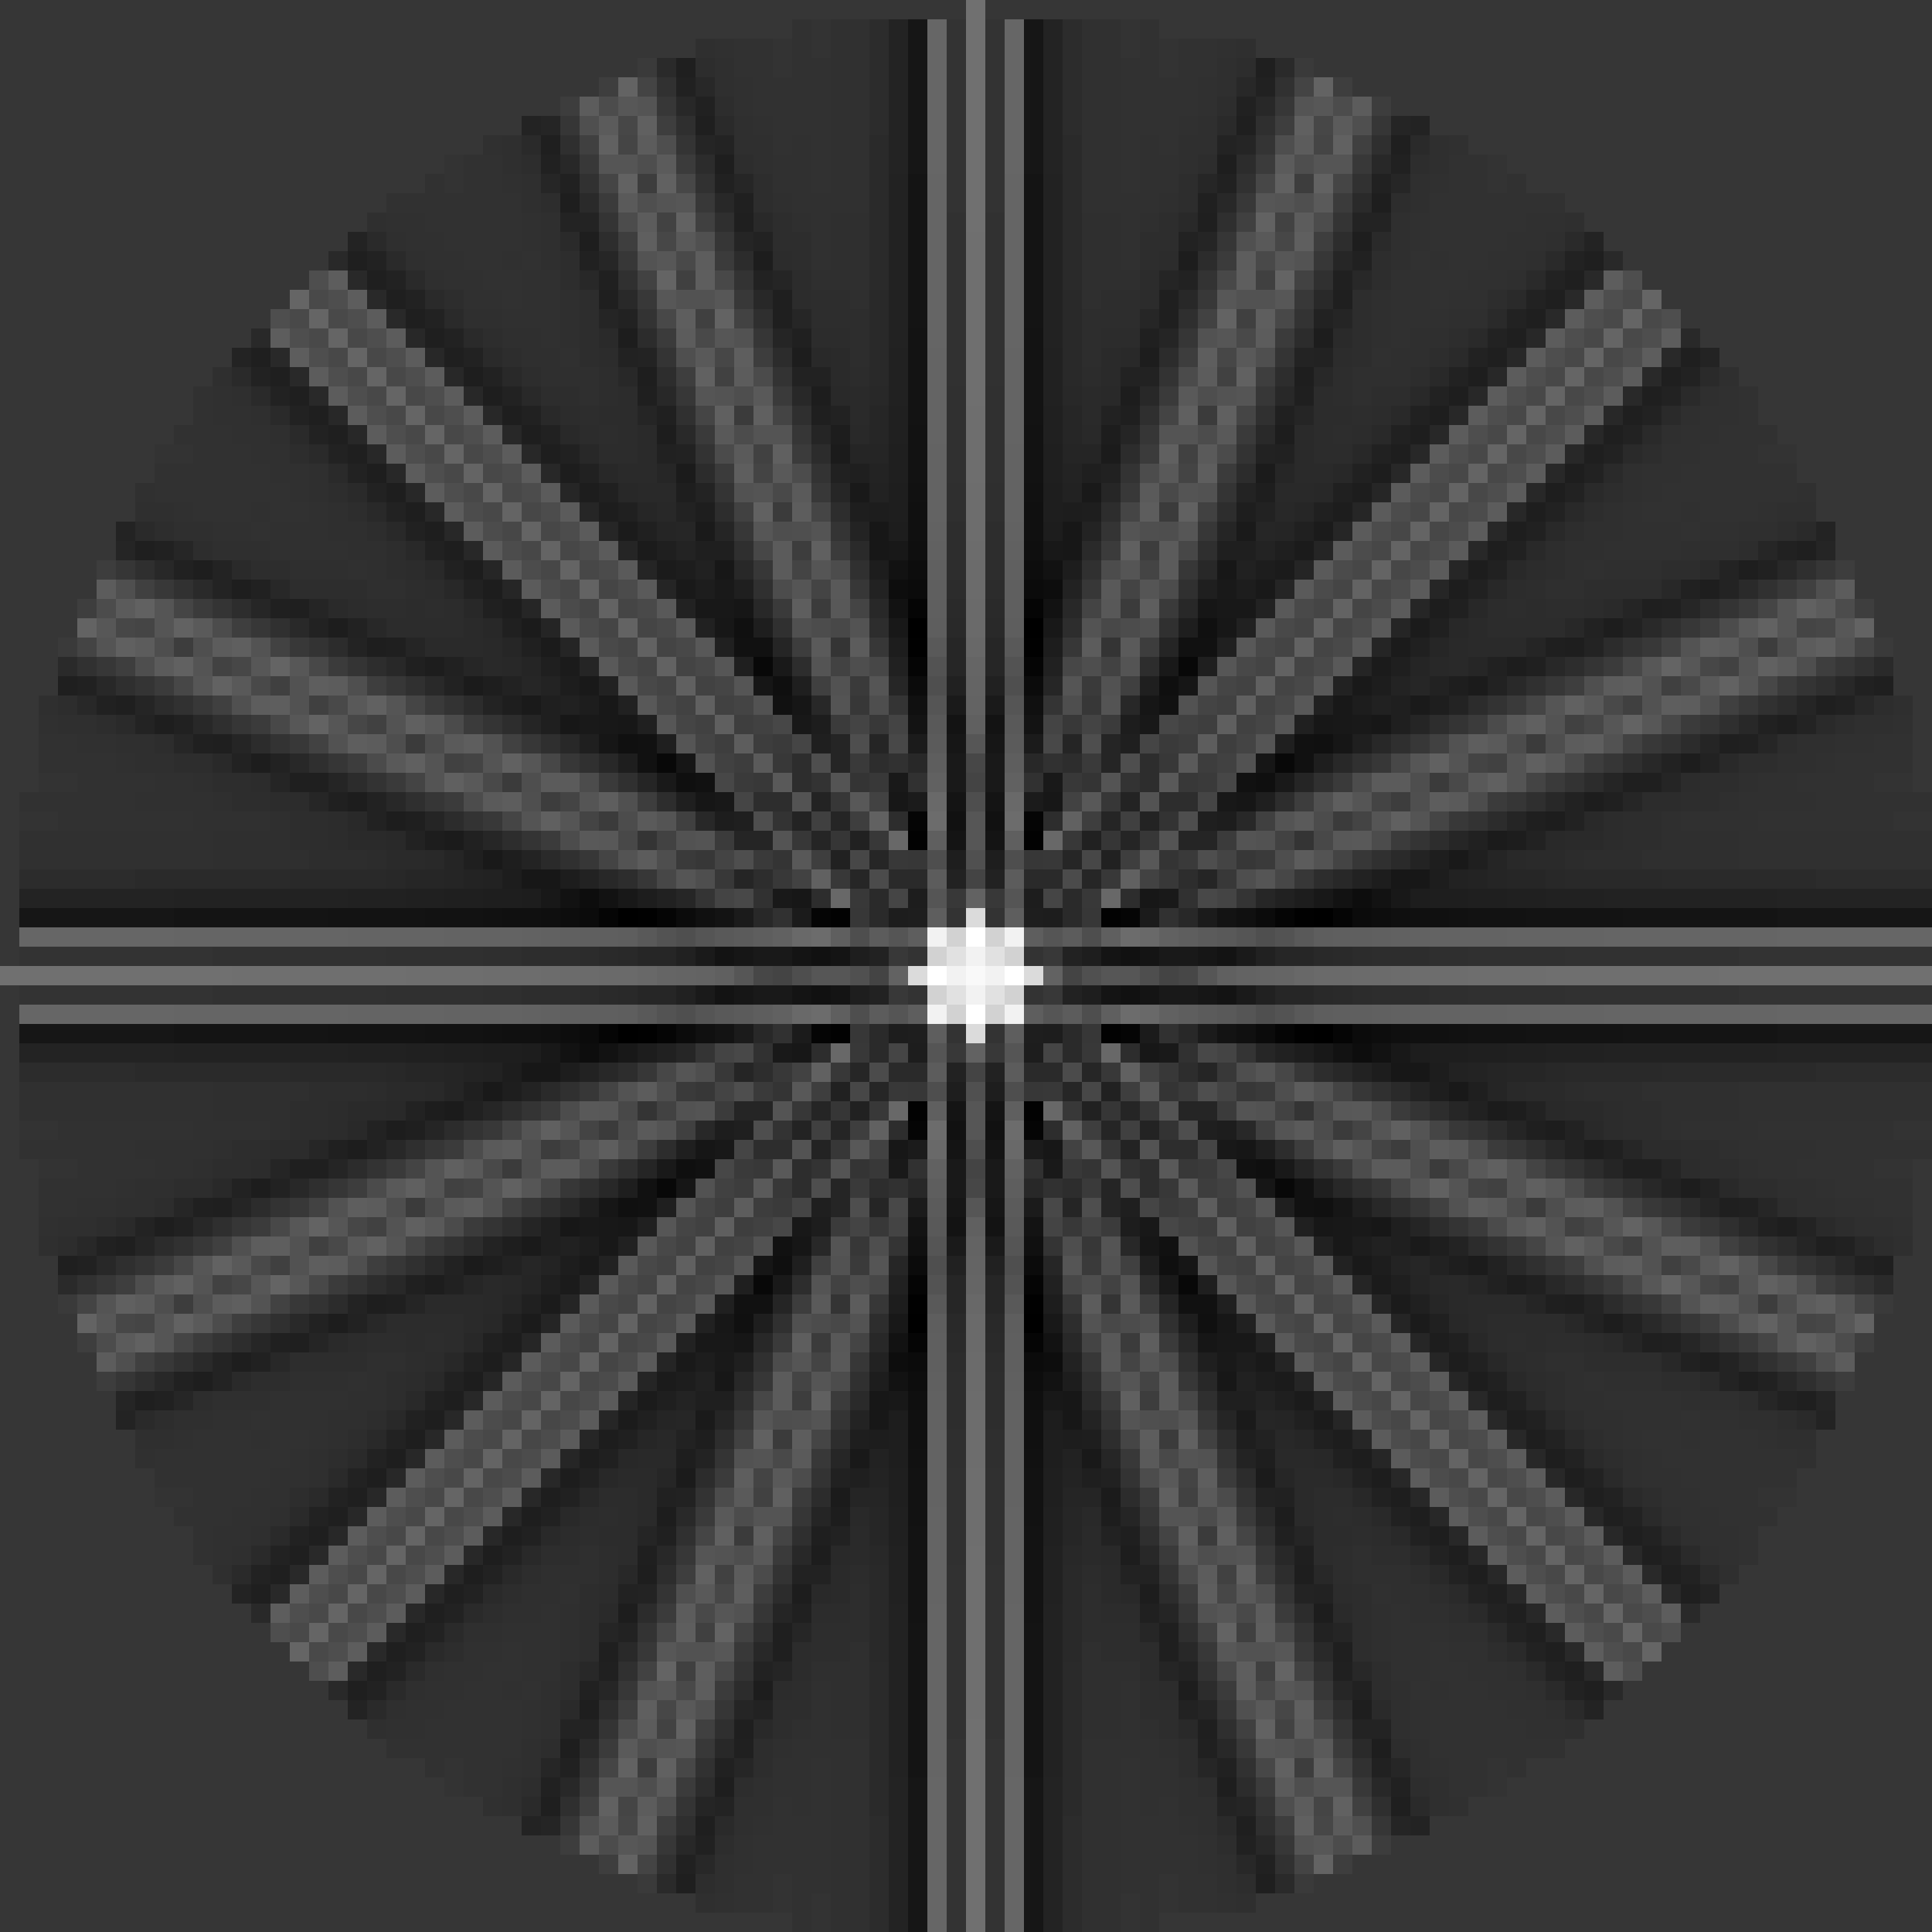
\includegraphics[width=\textwidth]{Figuras/retroproyeccion_p=16_filter=ramp.png}
           \caption{16 proyecciones.} 
        \end{subfigure}
        \begin{subfigure}[h]{0.24\textwidth}
           \centering
           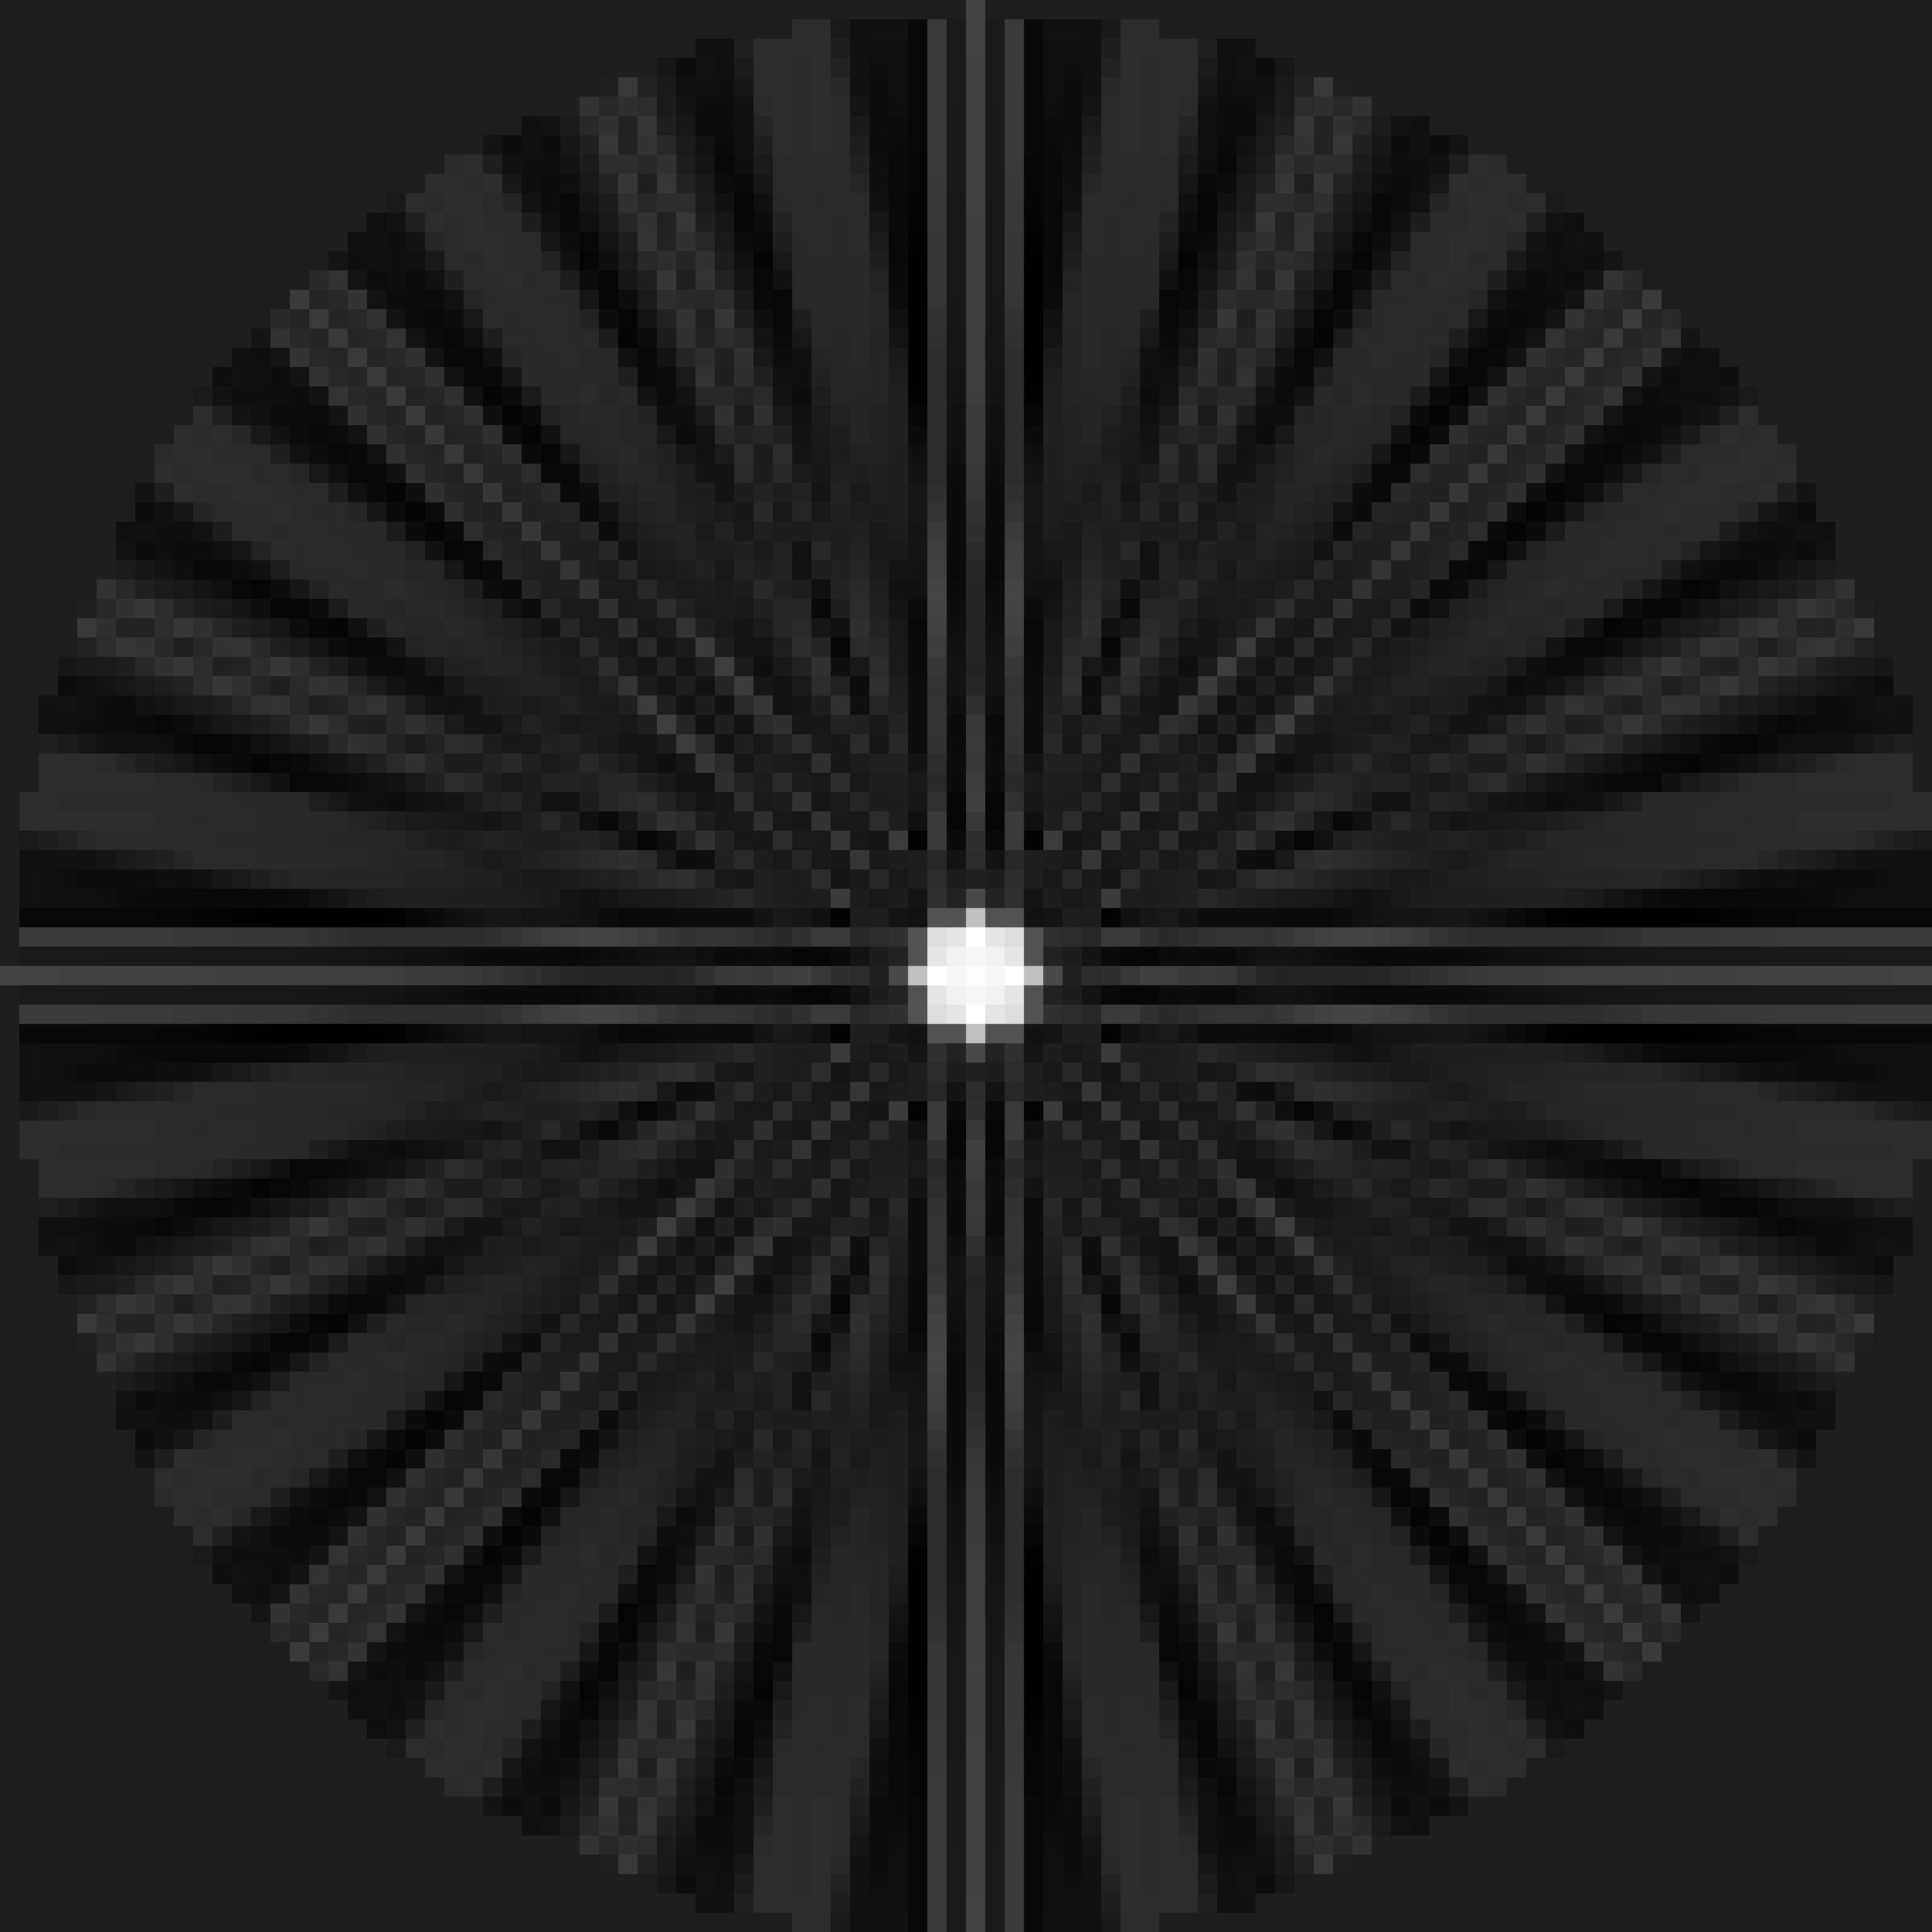
\includegraphics[width=\textwidth]{Figuras/retroproyeccion_p=32_filter=ramp.png}
           \caption{32 proyecciones.} 
        \end{subfigure}
        \begin{subfigure}[h]{0.24\textwidth}
           \centering
           
\includegraphics[width=\textwidth]{Figuras/retroproyeccion_p=64_filter=ramp.png}
           \caption{64 proyecciones.} 
        \end{subfigure}
   \caption{Retroproyeccion del círculo (Fig. \ref{fig:sinograma_circulo}) para 100 detectores y $8,16,32,64$ proyecciones. Arriba: Retroproyección sin filtro. Abajo: Retroproyección con filtro rampa.}
   \label{fig:retroproyeccion_circulo}
\end{figure}

\section{Defecto de un detector}

En esta sección se estudiará qué sucede cuando un detector del equipo no registra ninguna actividad. En primer lugar, este defecto se traduce en el sinograma como una columna oscura ya que en el eje horizontal se grafican el número de detectores. En la parte superior de la Fig. \ref{fig:detector_roto} se muestran sinogramas generados con 367 detectores y 320 proyecciones recorriendo media circunferencia con defectos en los detectores 50, 150, 250 y 300. En la parte inferior de la Fig. \ref{fig:detector_roto} se muestran las retroproyecciones filtradas con filtro rampa de los sinogramas con defectos. Se observa que, en todos los casos, se obtiene un artefacto semicircular de radio igual a la distancia del centro de la imagen a la columna sin señal en el sinograma. Además, se observan dos líneas tangentes a los extremos del semicírculo. 

Notar que en el caso \ref{fig:sinograma_50}, la columna se encuentra parcialmente dentro del sinograma. En este caso, las líneas tangentes no son verticales como sucede en los otros tres casos donde los defectos están totalmente contenidos en la imagen. 

\begin{figure}[H]
   \centering
       \begin{subfigure}[h]{0.24\textwidth}
           \centering
           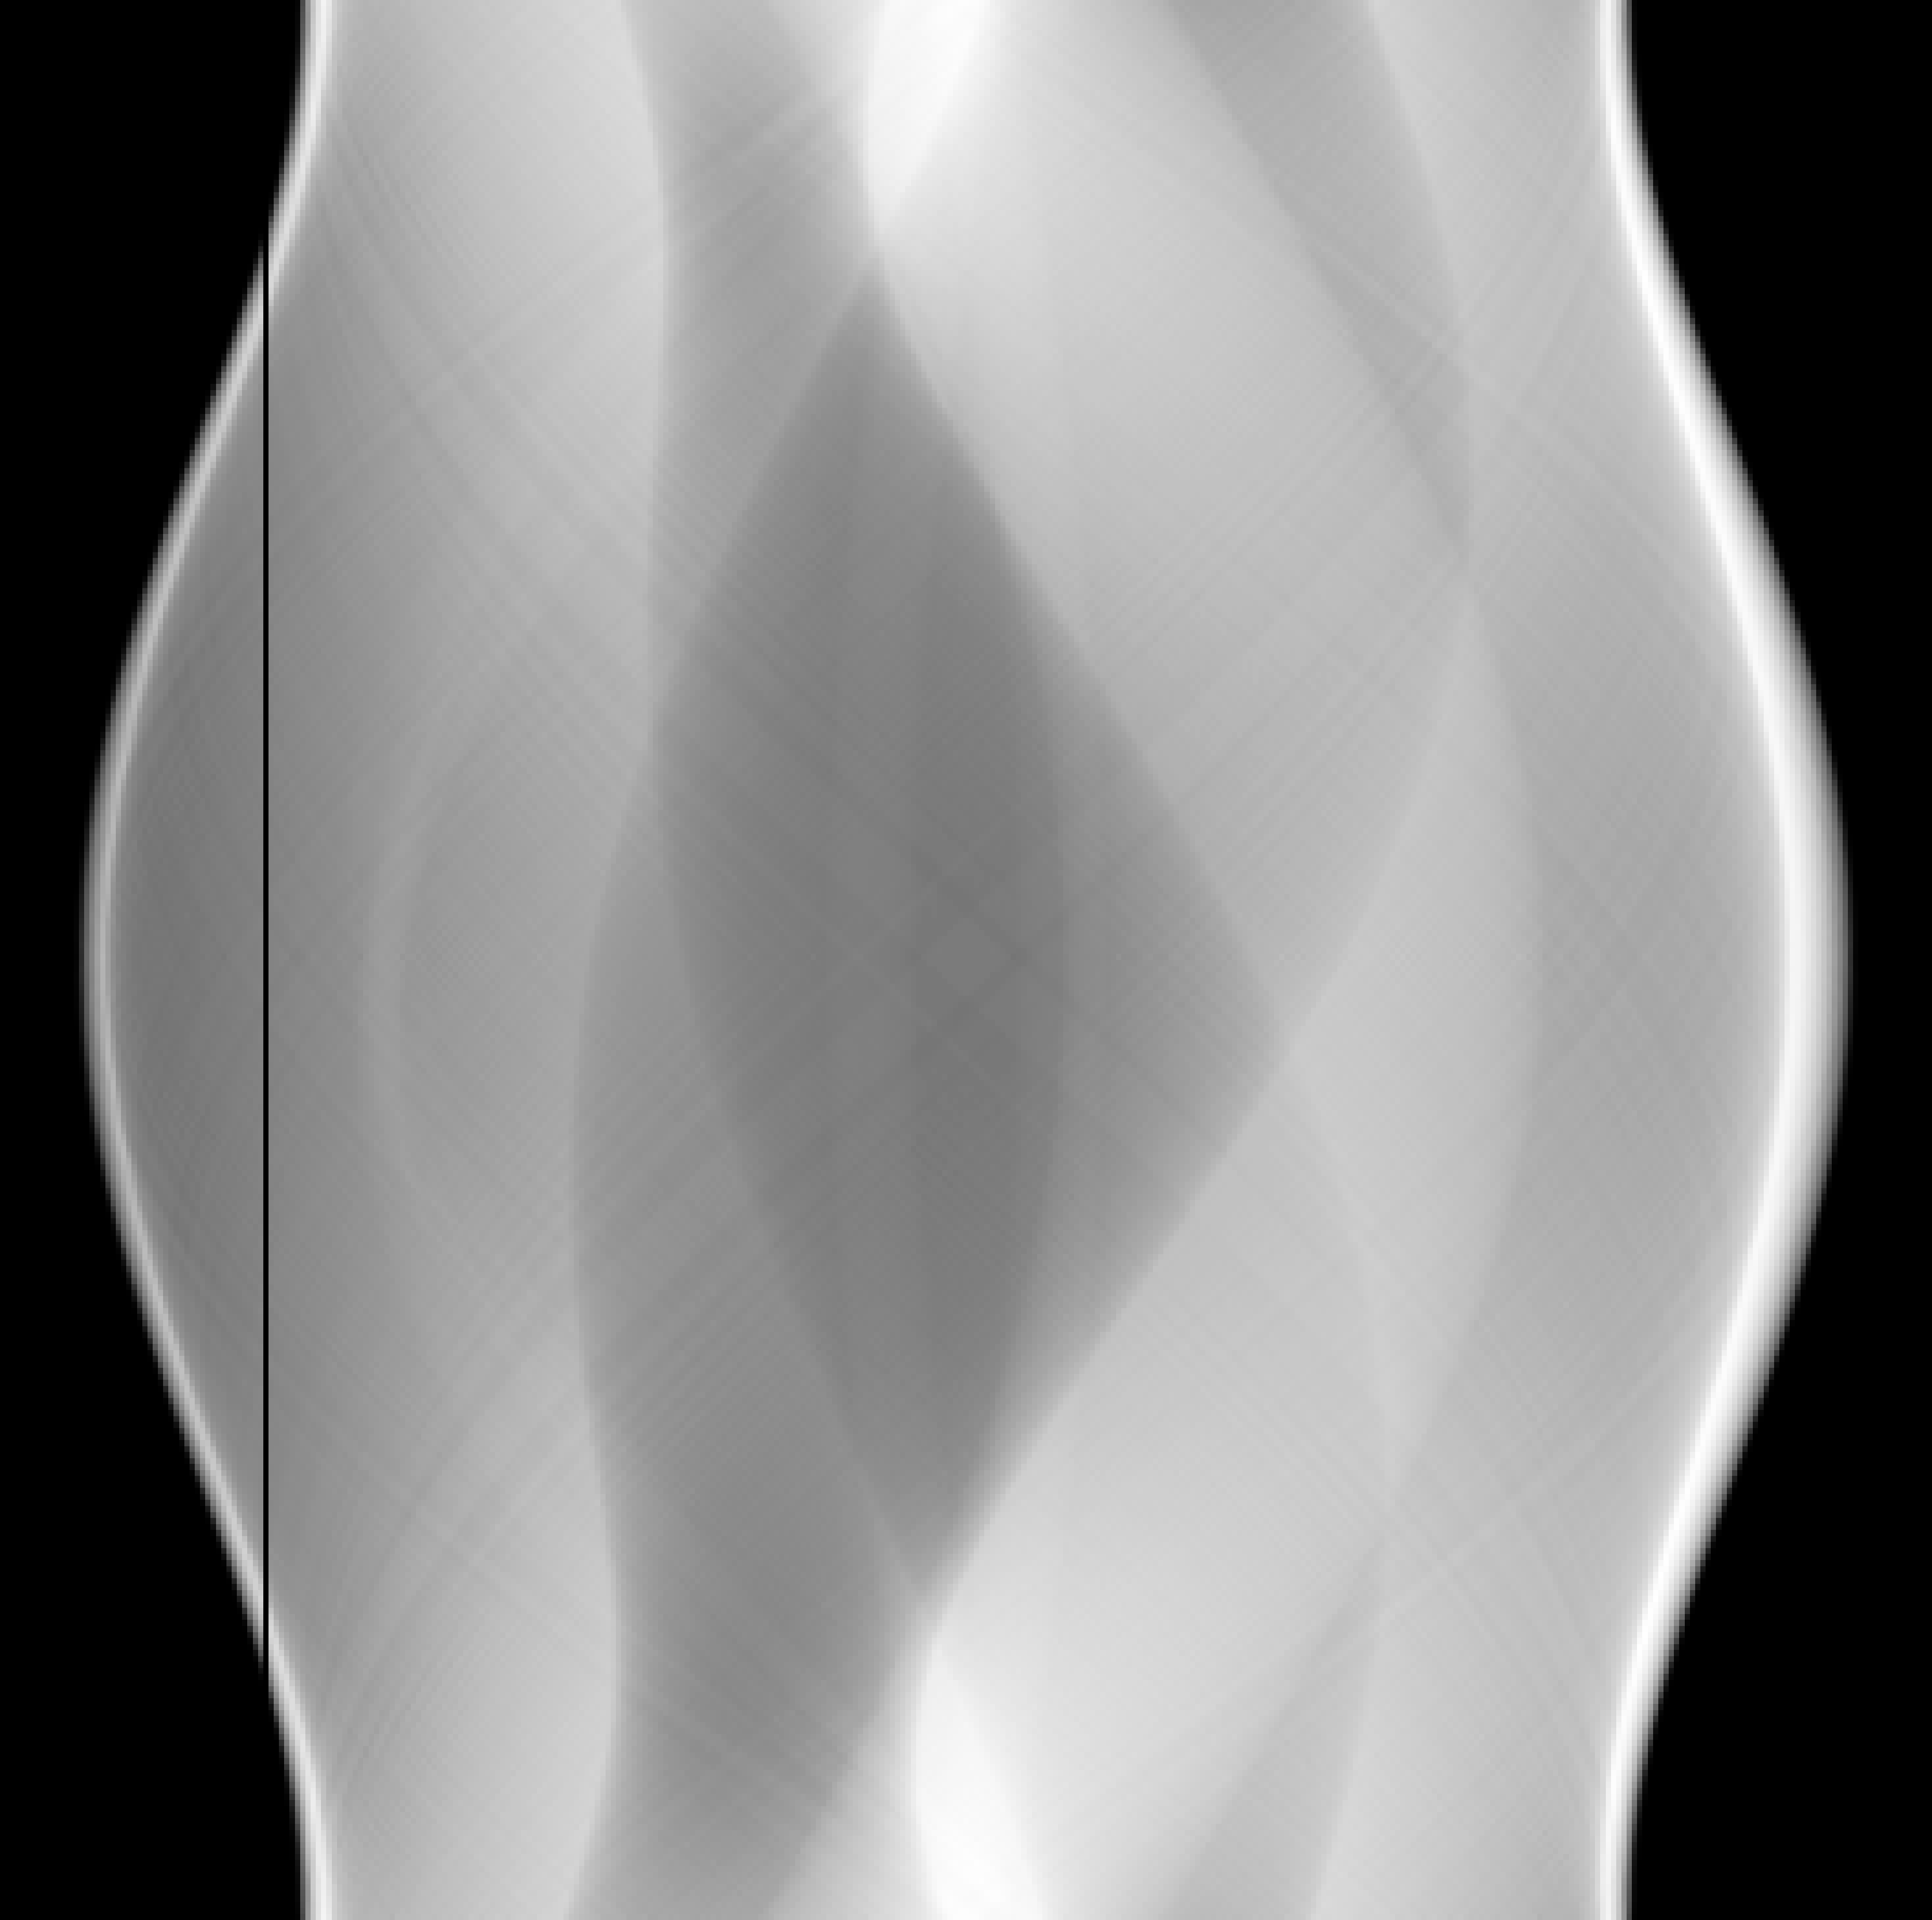
\includegraphics[width=\textwidth]{Figuras/sinograma_50.png} 
       \end{subfigure}
       \begin{subfigure}[h]{0.24\textwidth}
           \centering
           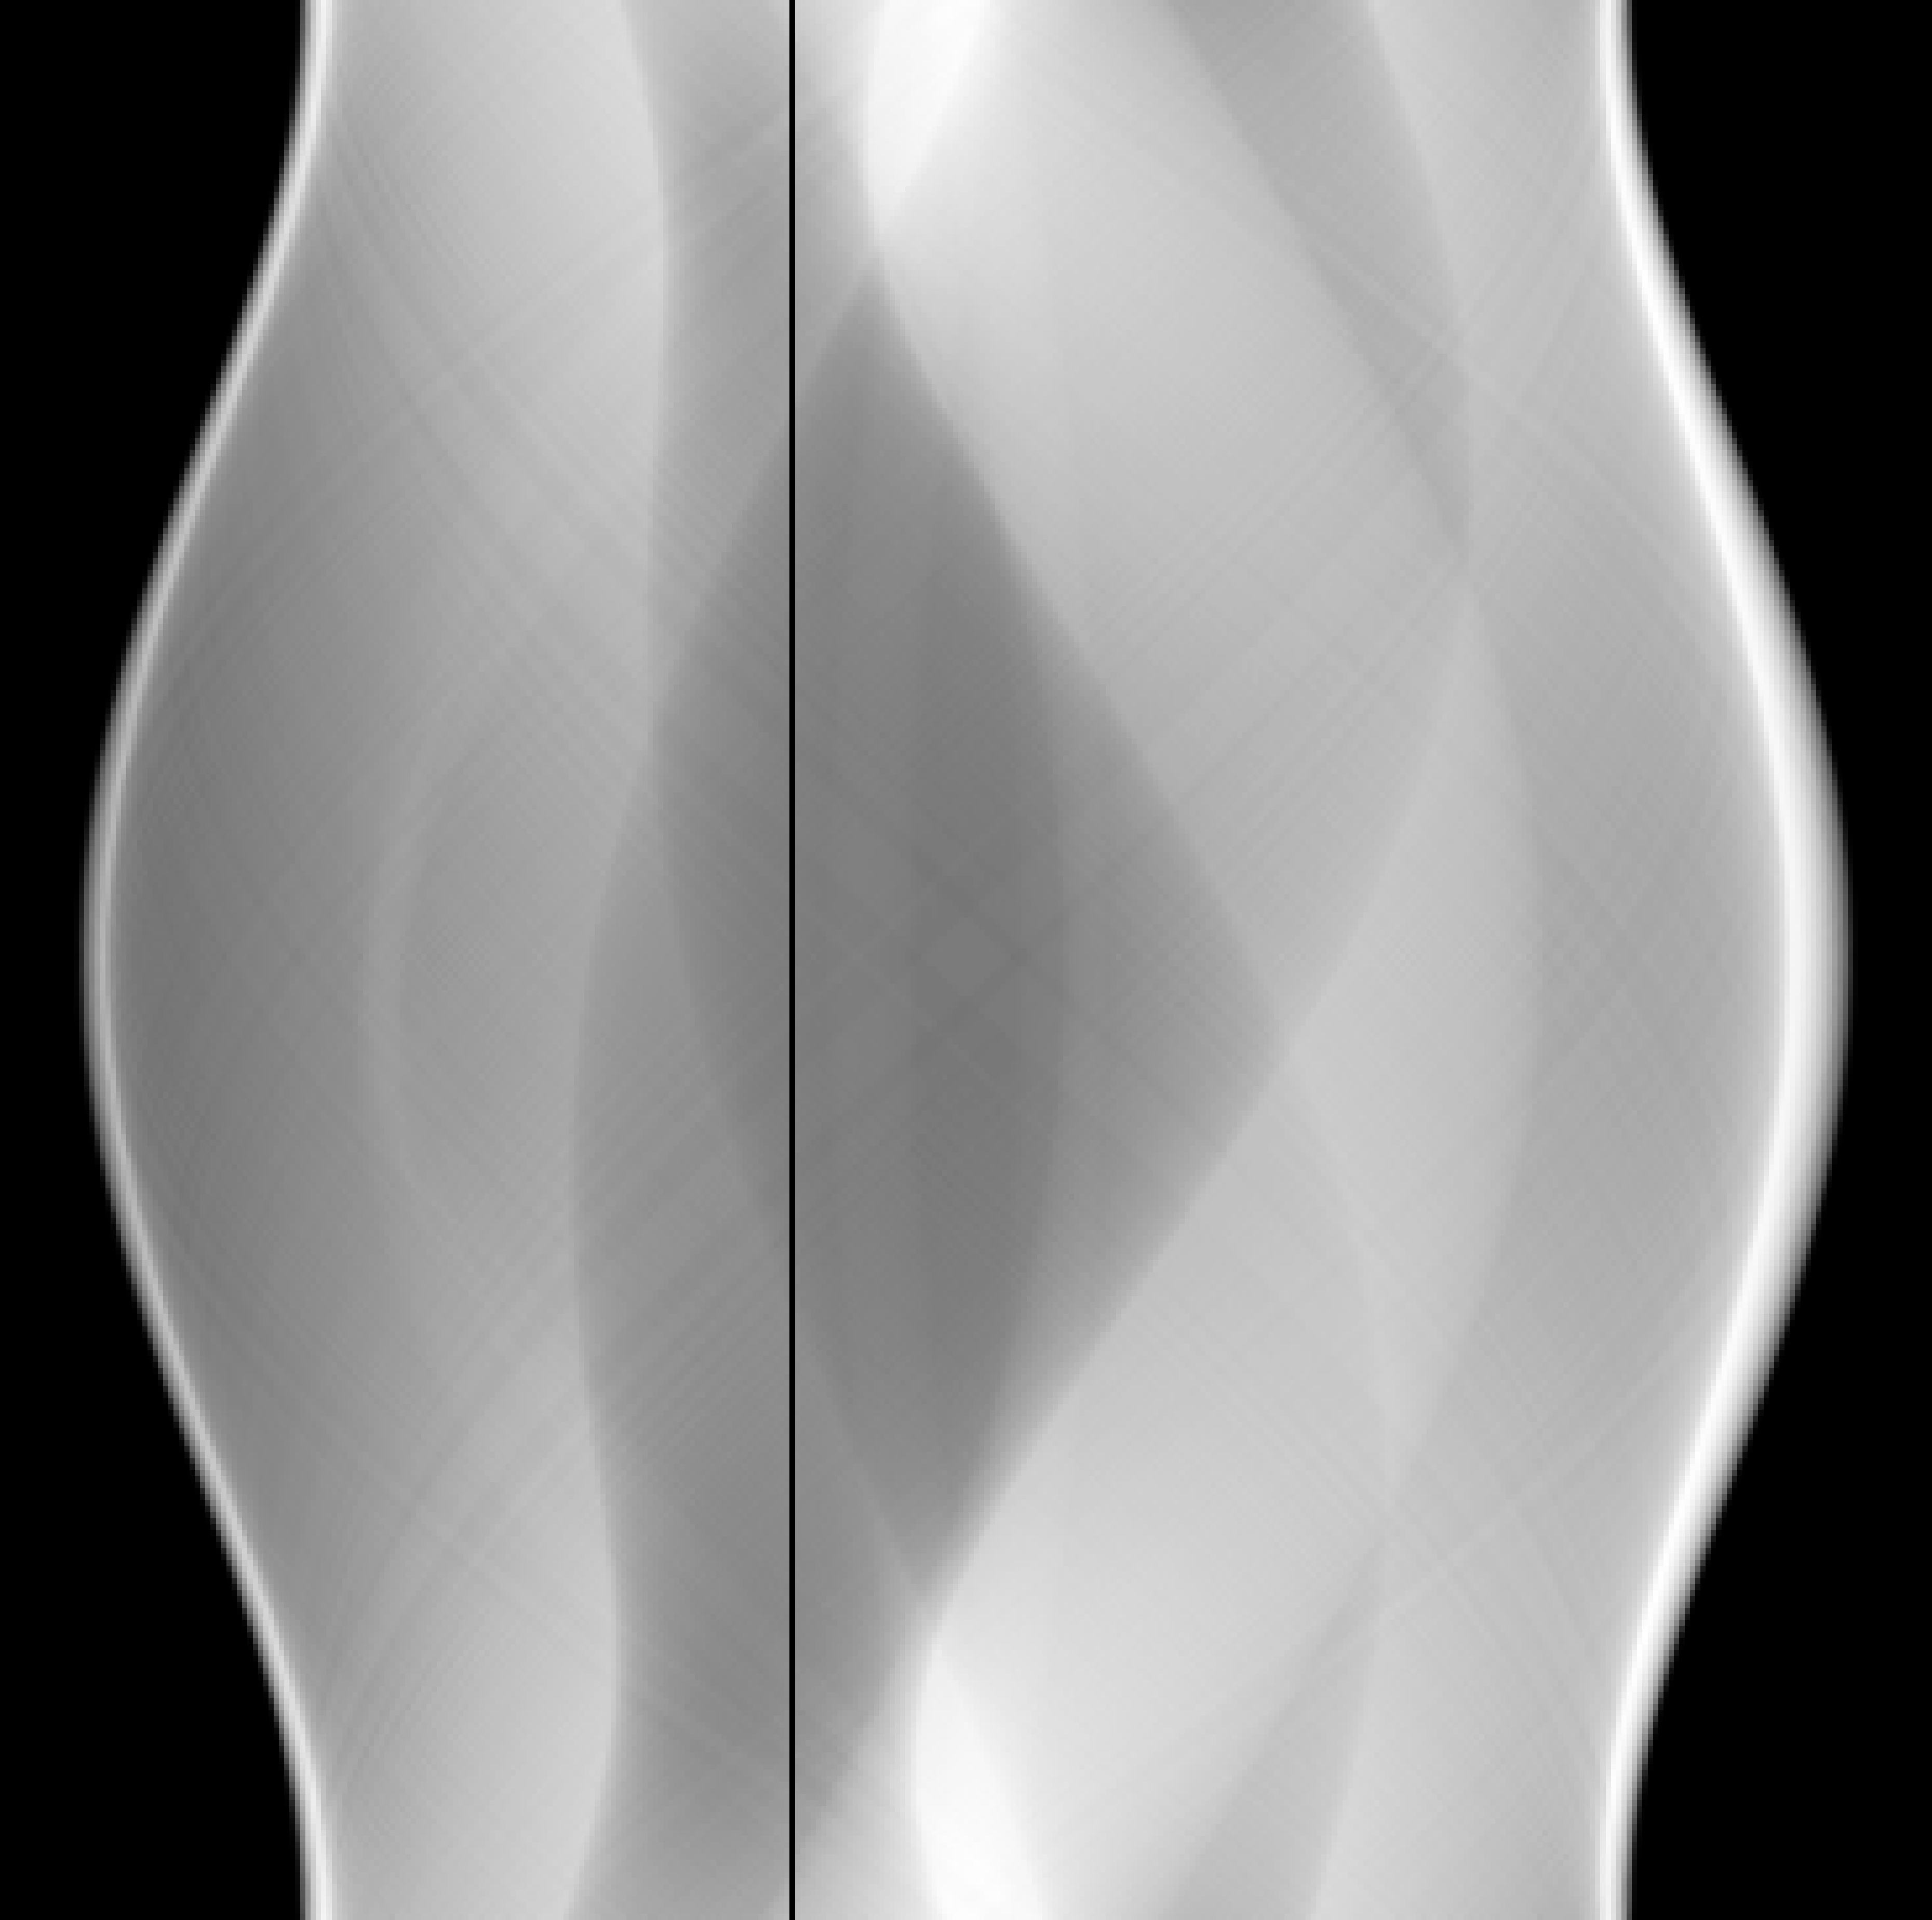
\includegraphics[width=\textwidth]{Figuras/sinograma_150.png}
       \end{subfigure}
       \begin{subfigure}[h]{0.24\textwidth}
           \centering
           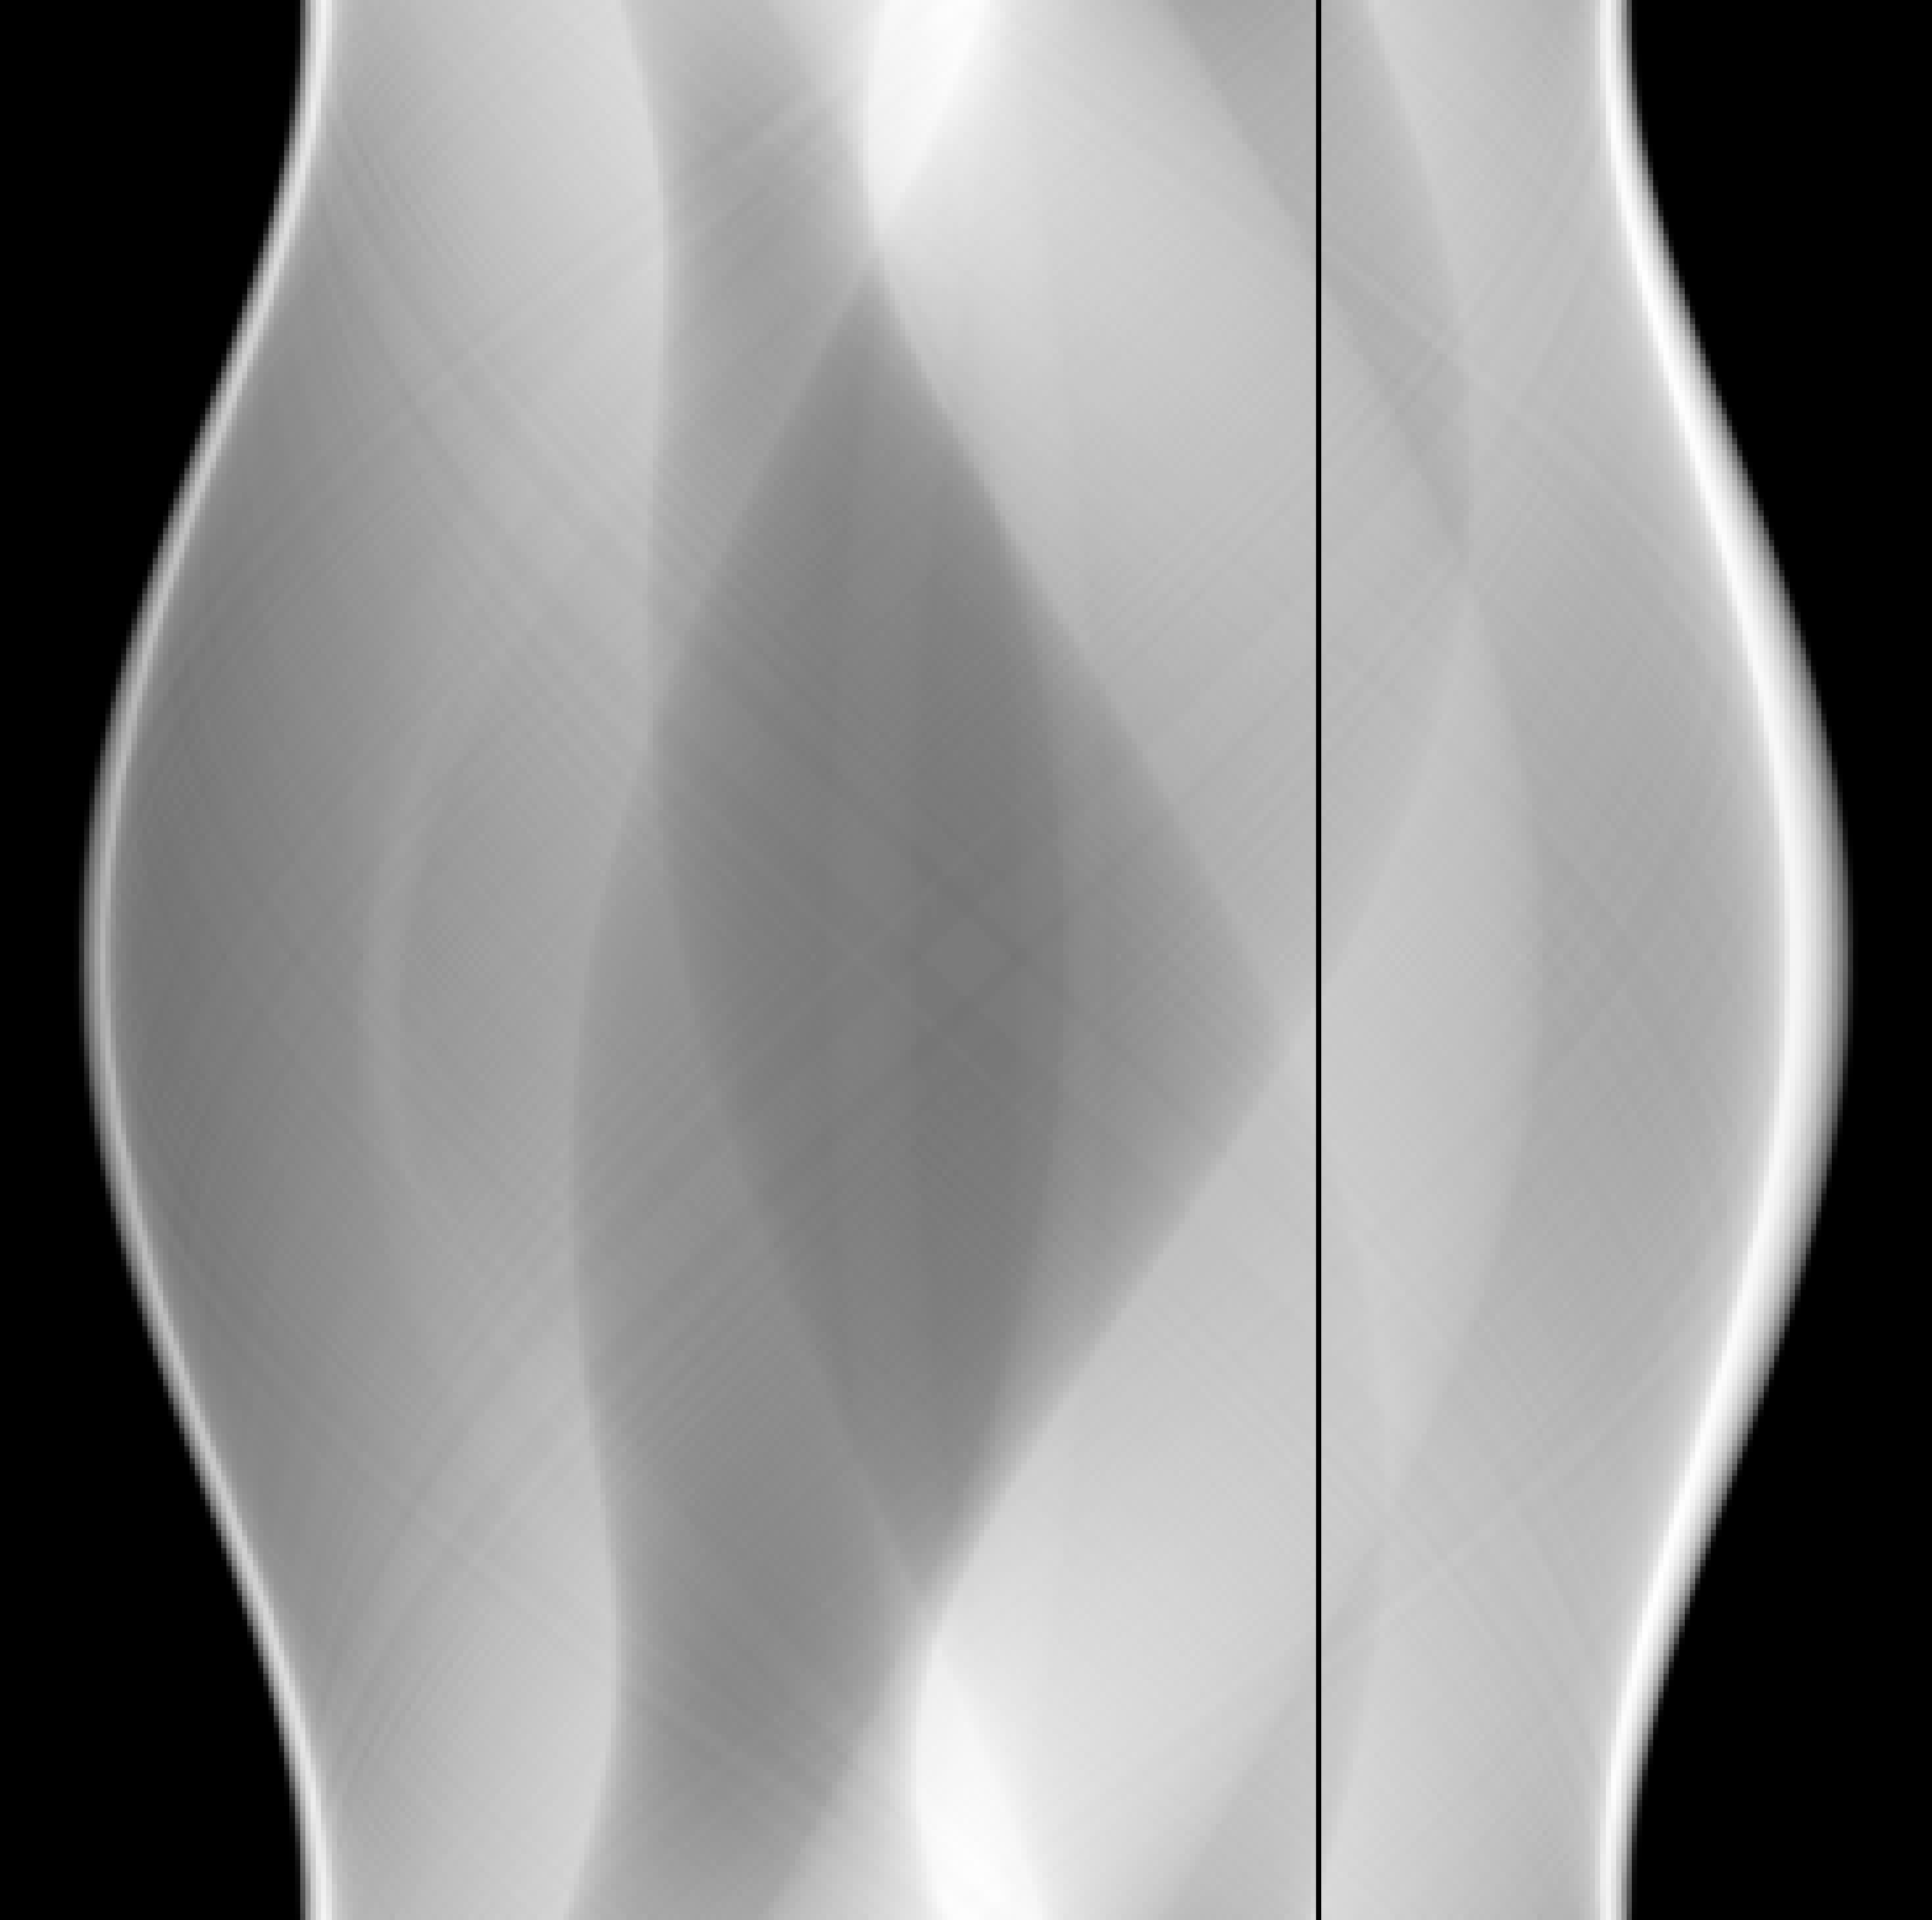
\includegraphics[width=\textwidth]{Figuras/sinograma_250.png}
       \end{subfigure}
       \begin{subfigure}[h]{0.24\textwidth}
           \centering
           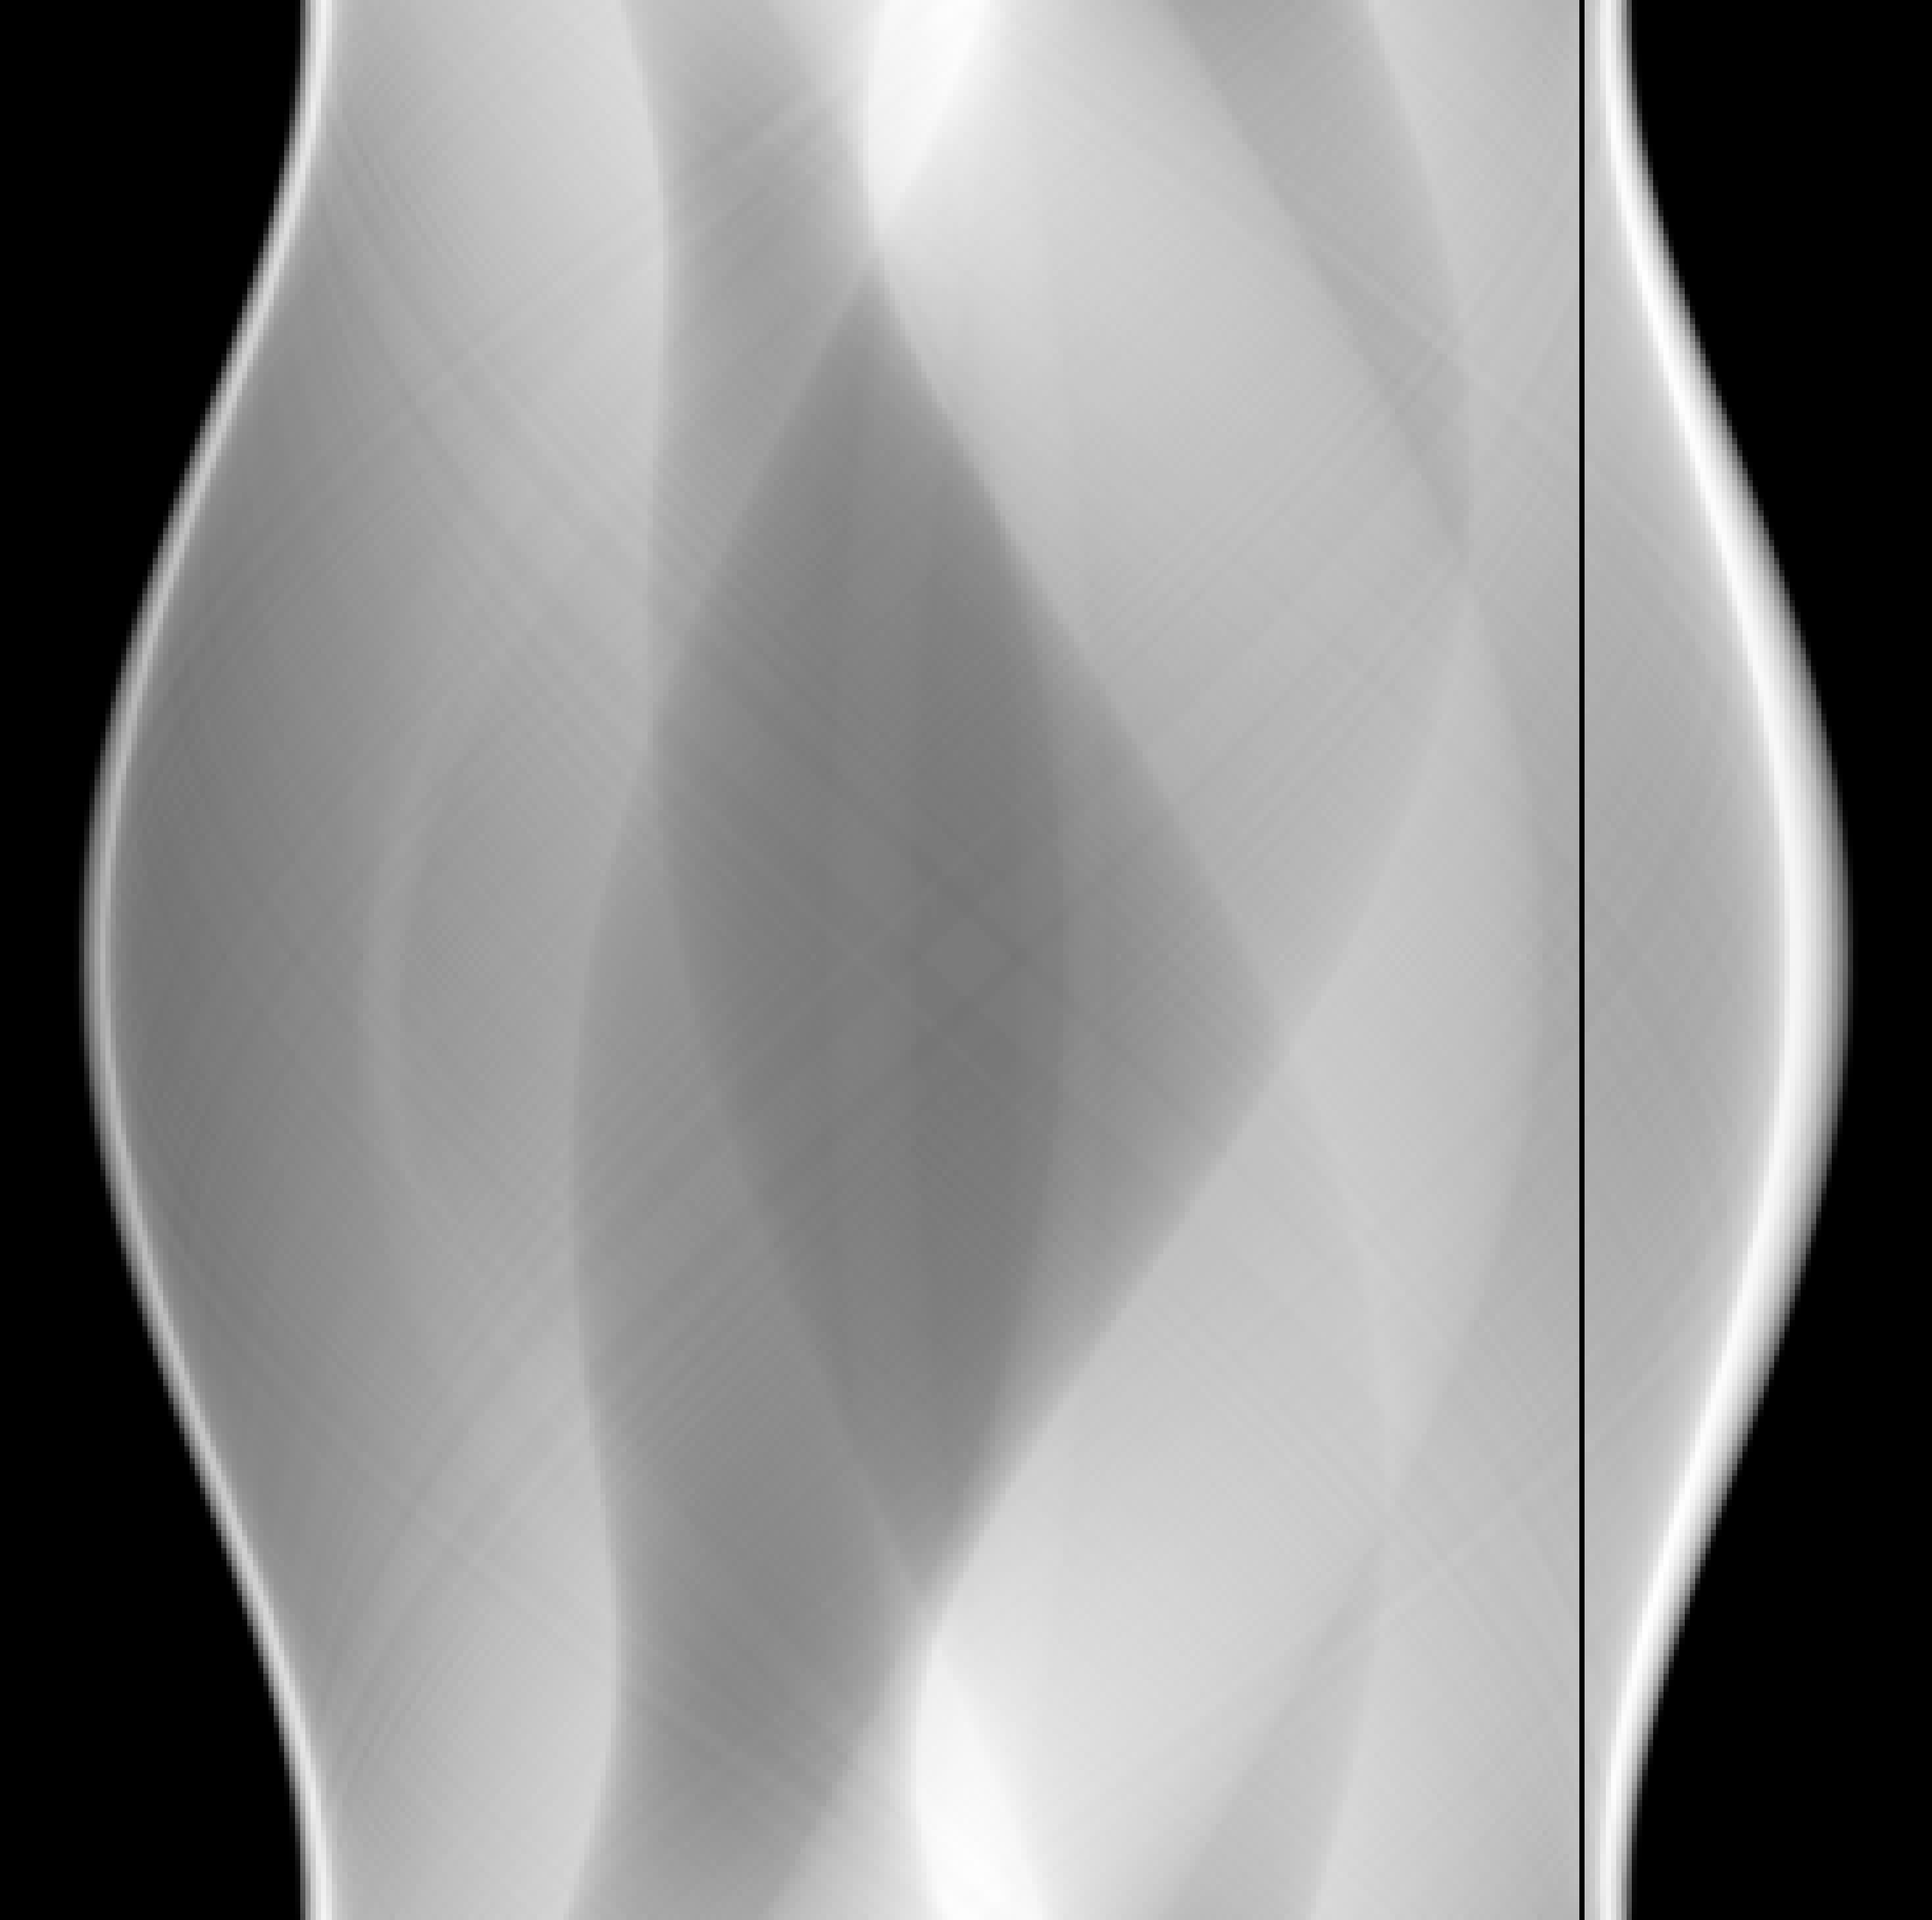
\includegraphics[width=\textwidth]{Figuras/sinograma_300.png}
       \end{subfigure}
        \begin{subfigure}[h]{0.24\textwidth}
           \centering
           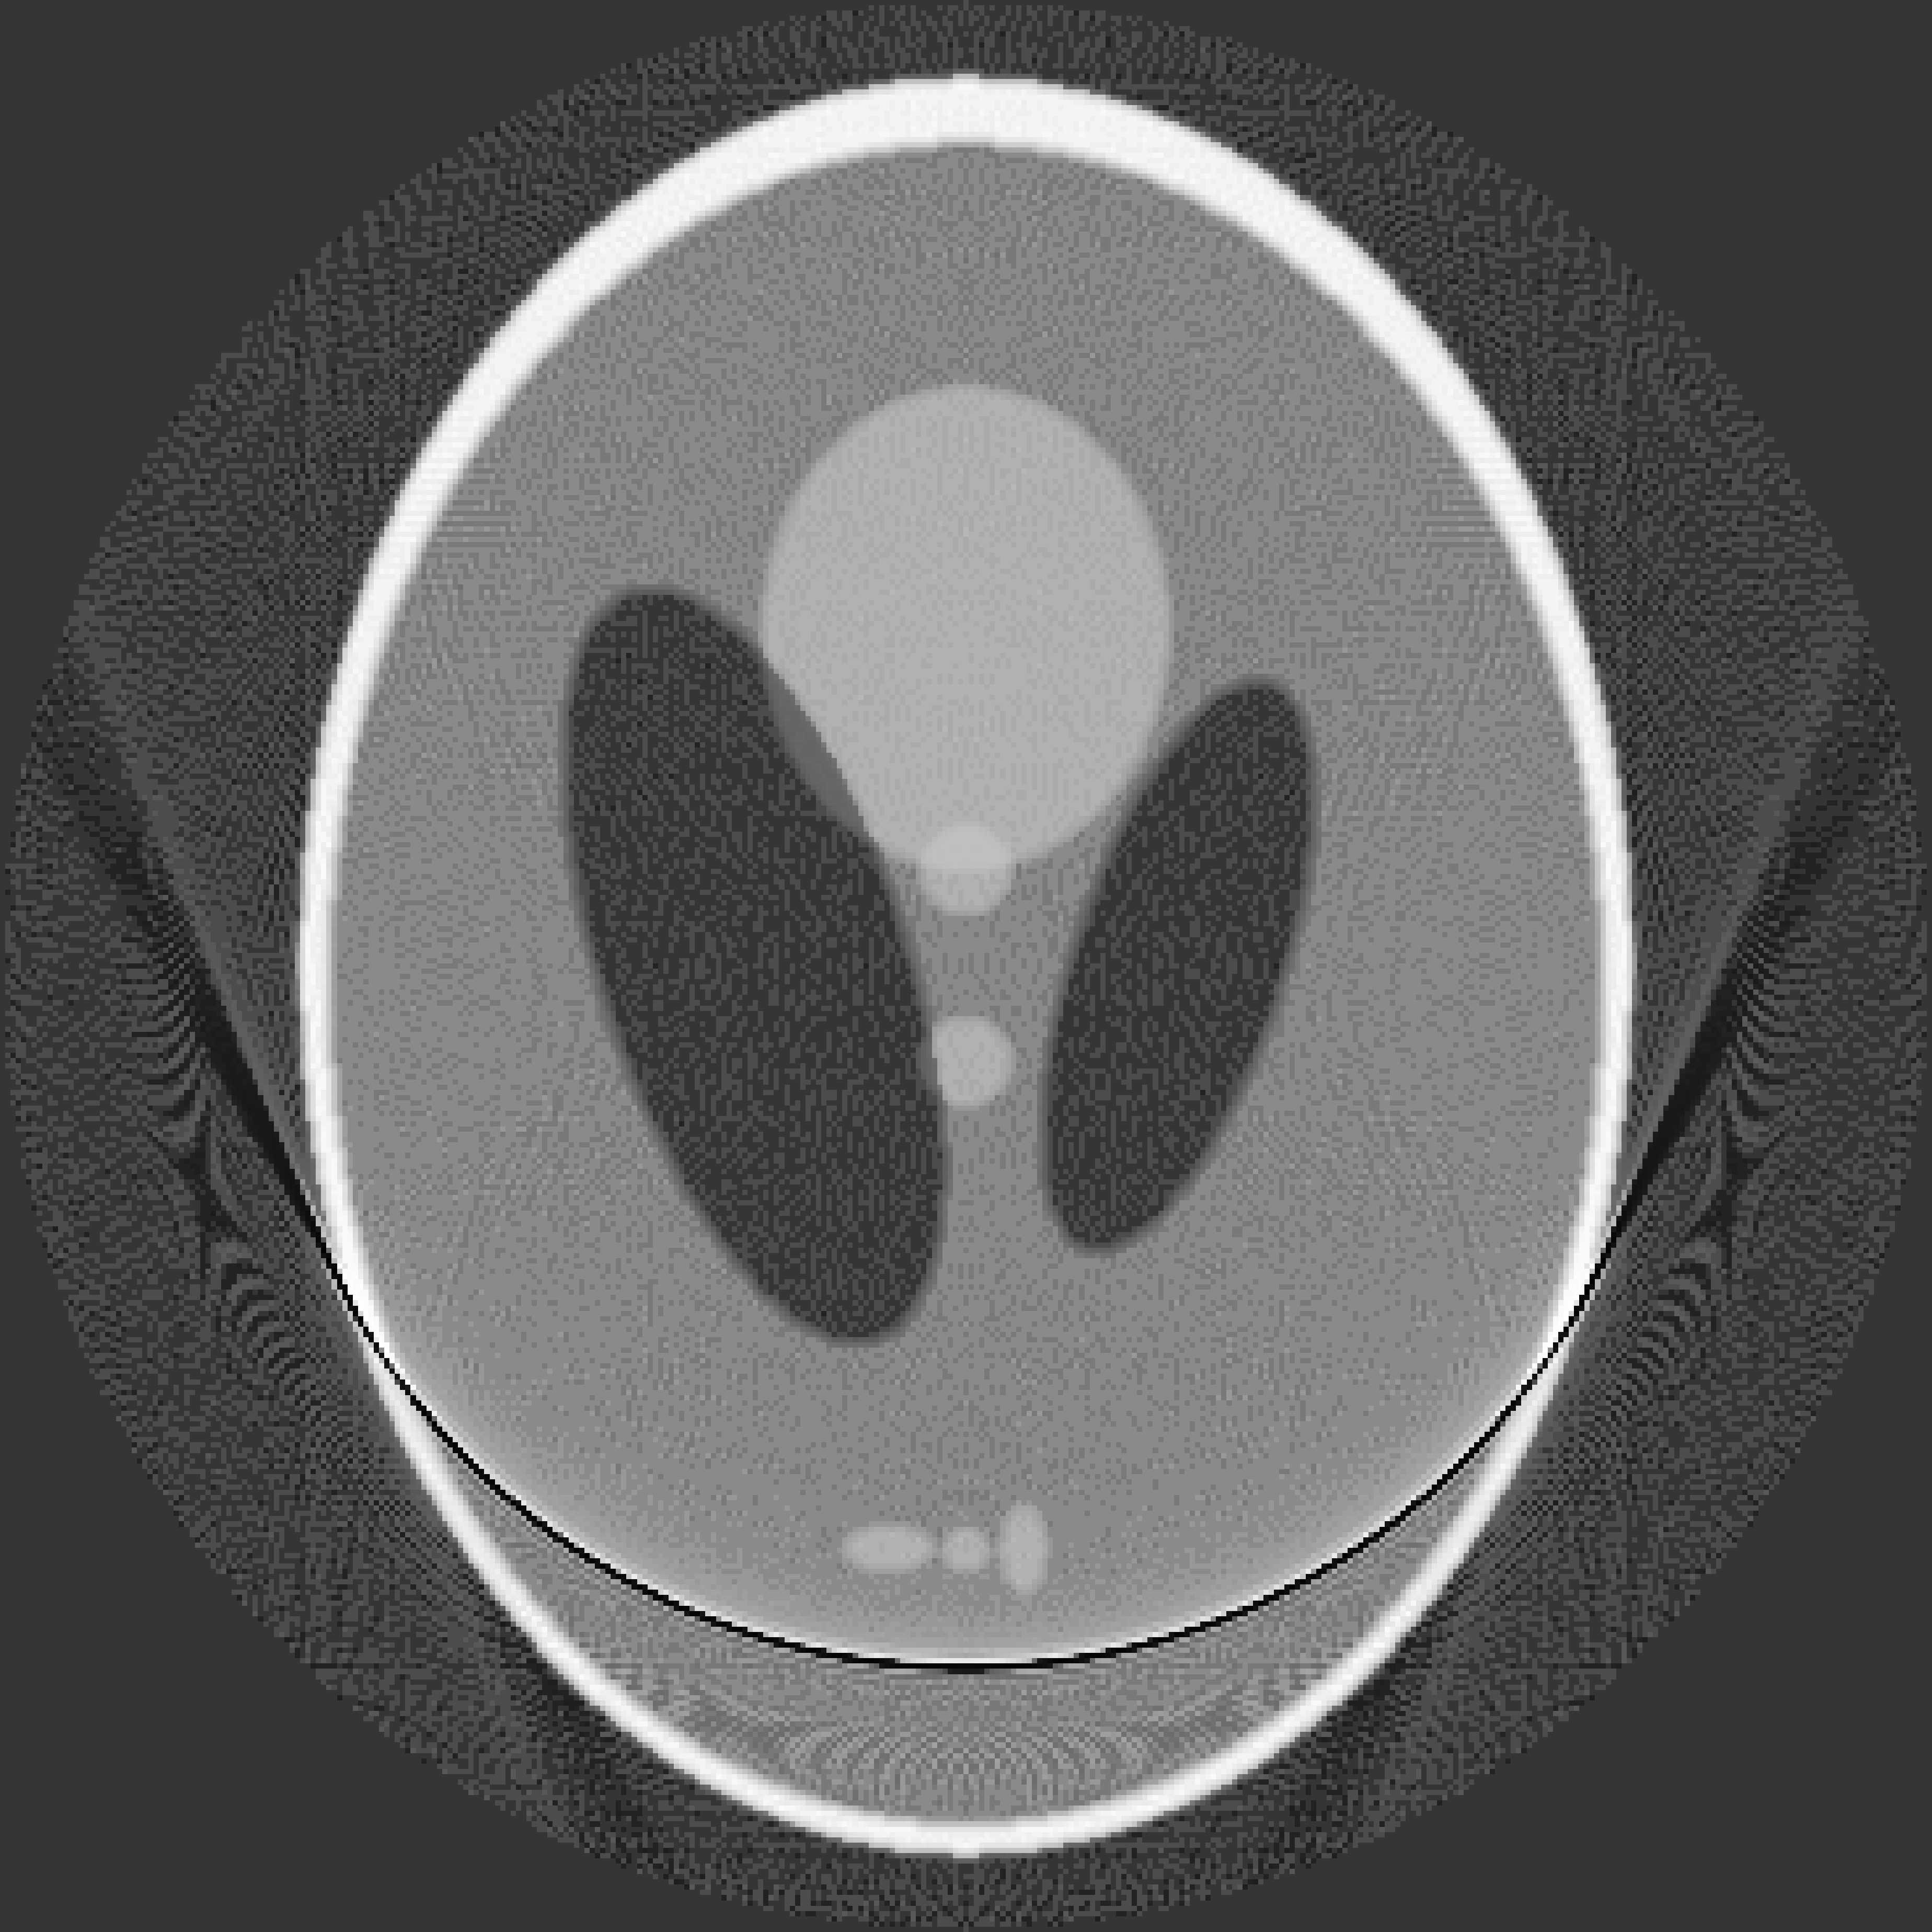
\includegraphics[width=\textwidth]{Figuras/reconstruction_50_EQ.png}
           \caption{Detector 50 defectuoso.} 
           \label{fig:sinograma_50}
        \end{subfigure}
        \begin{subfigure}[h]{0.24\textwidth}
           \centering
           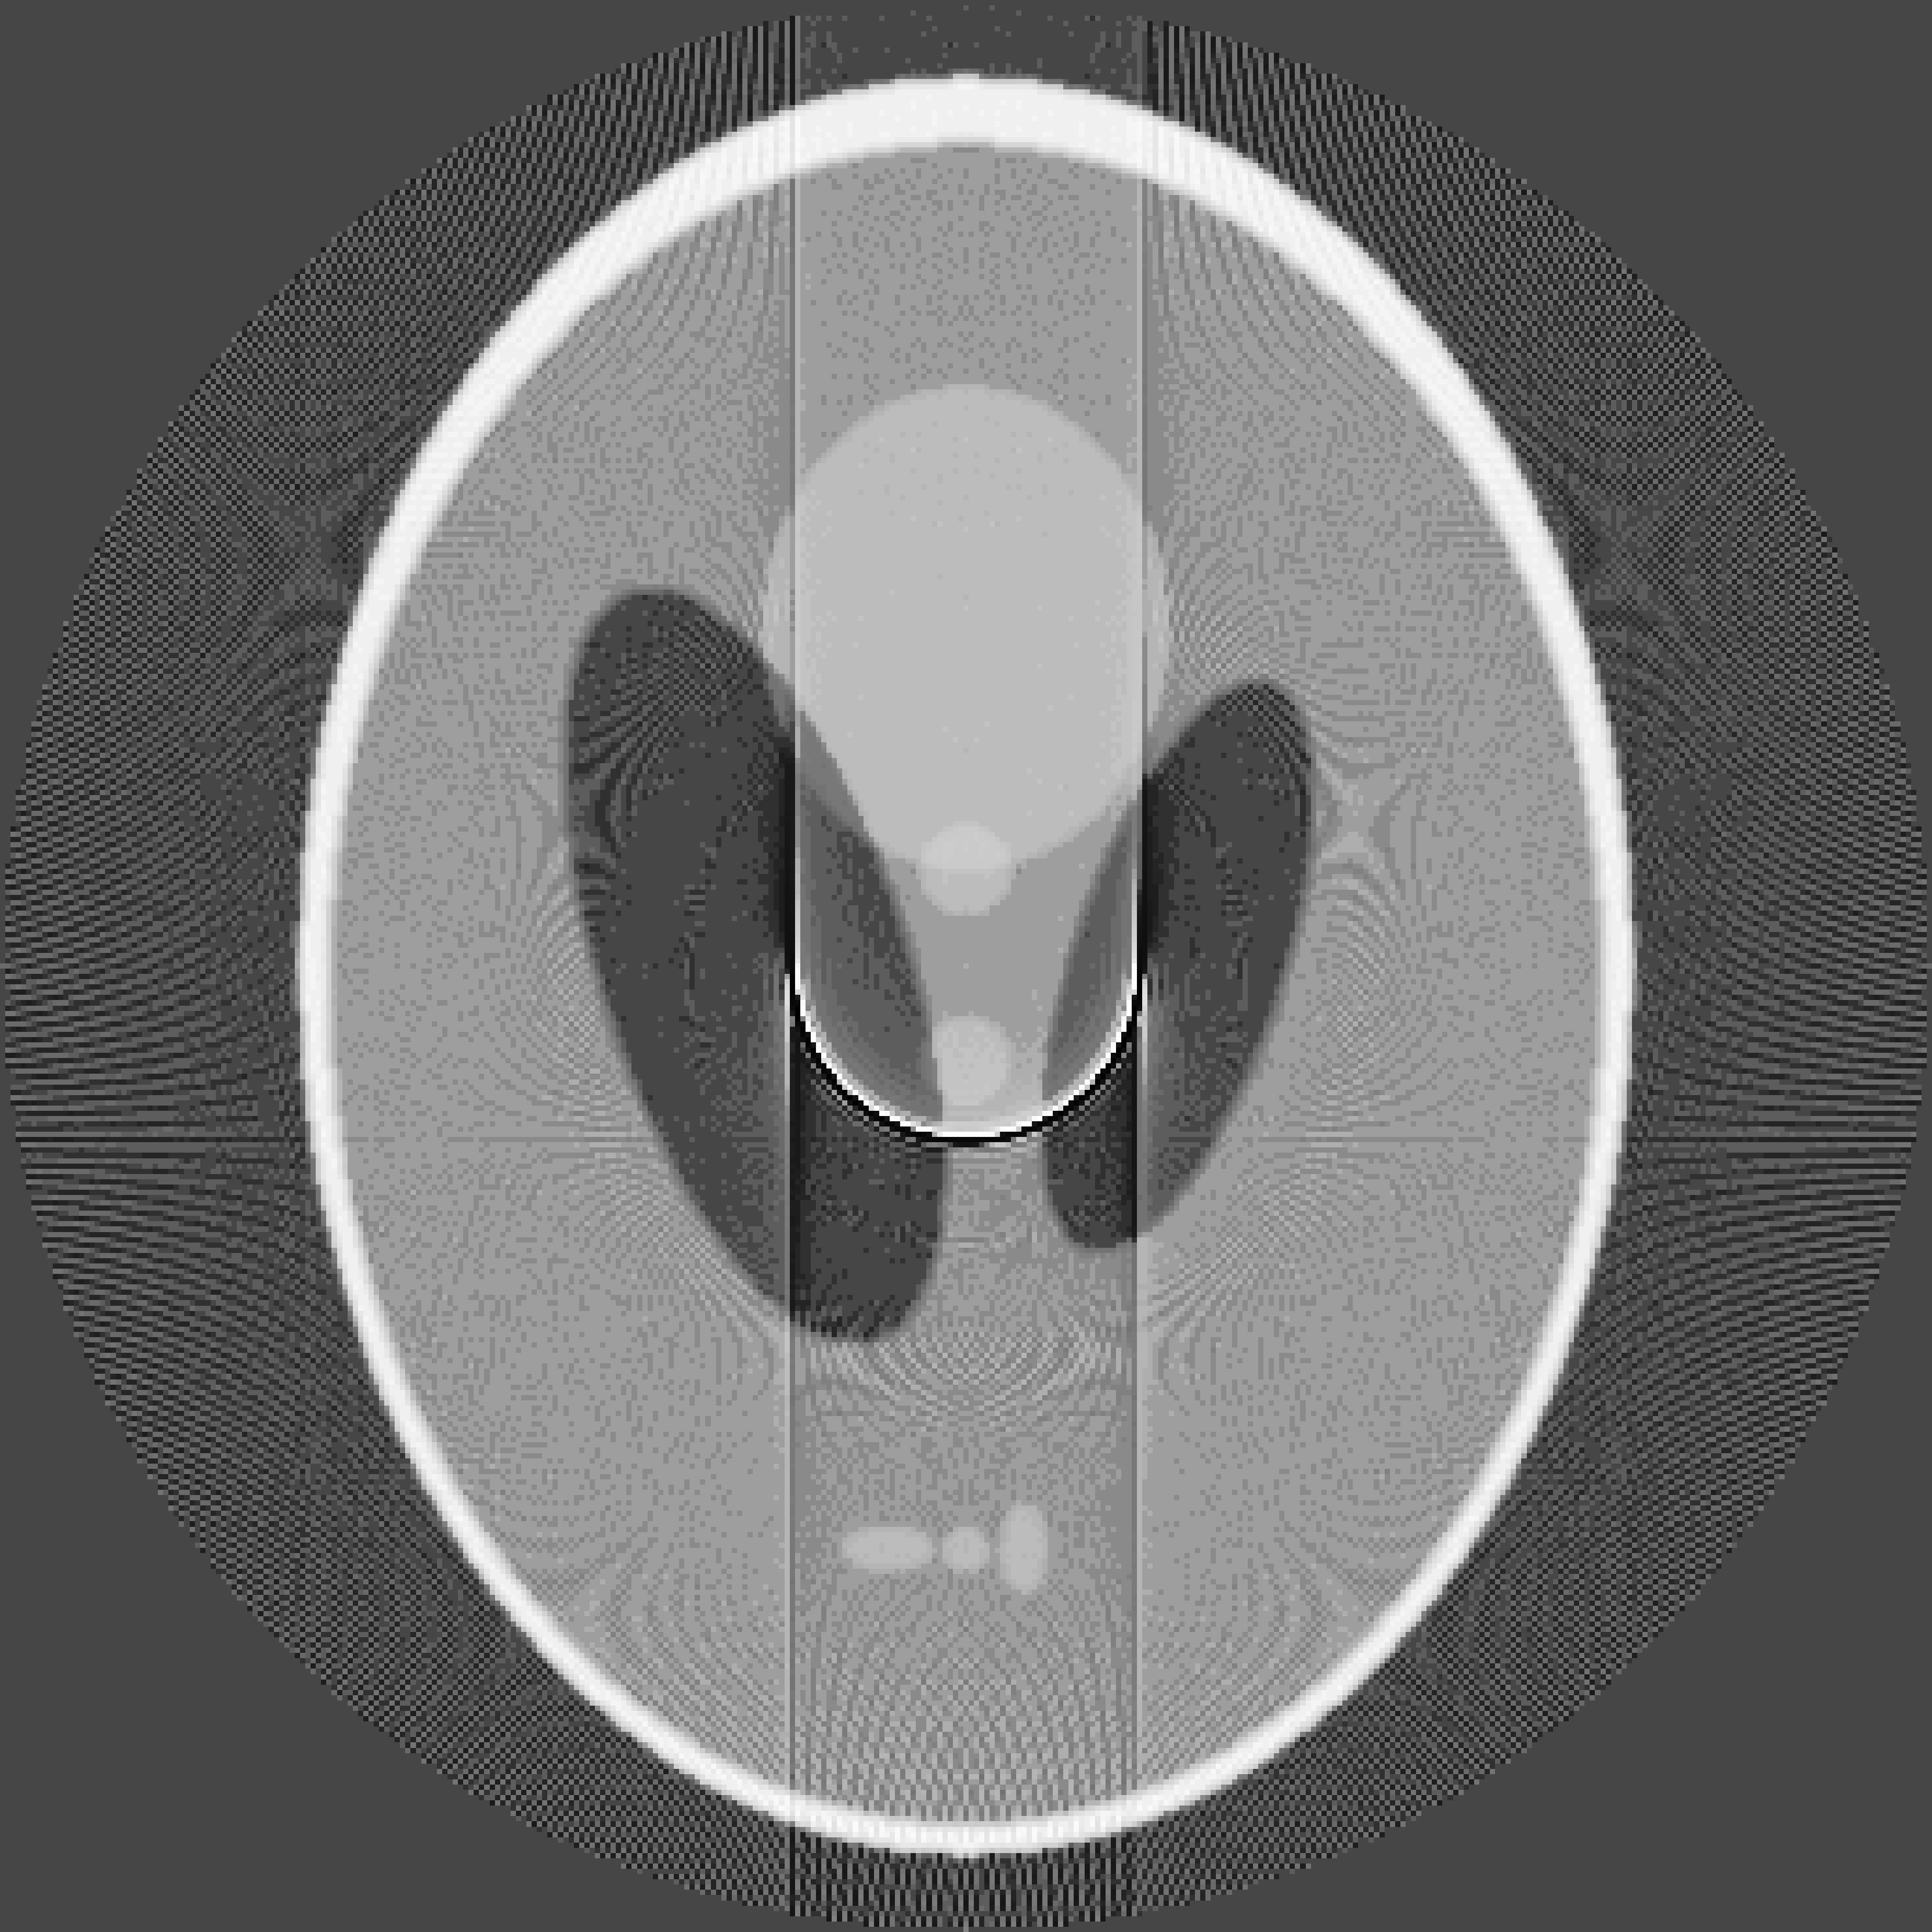
\includegraphics[width=\textwidth]{Figuras/reconstruction_150_EQ.png}
           \caption{Detector 150 defectuoso.} 
           \label{fig:sinograma_150}
        \end{subfigure}
        \begin{subfigure}[h]{0.24\textwidth}
           \centering
           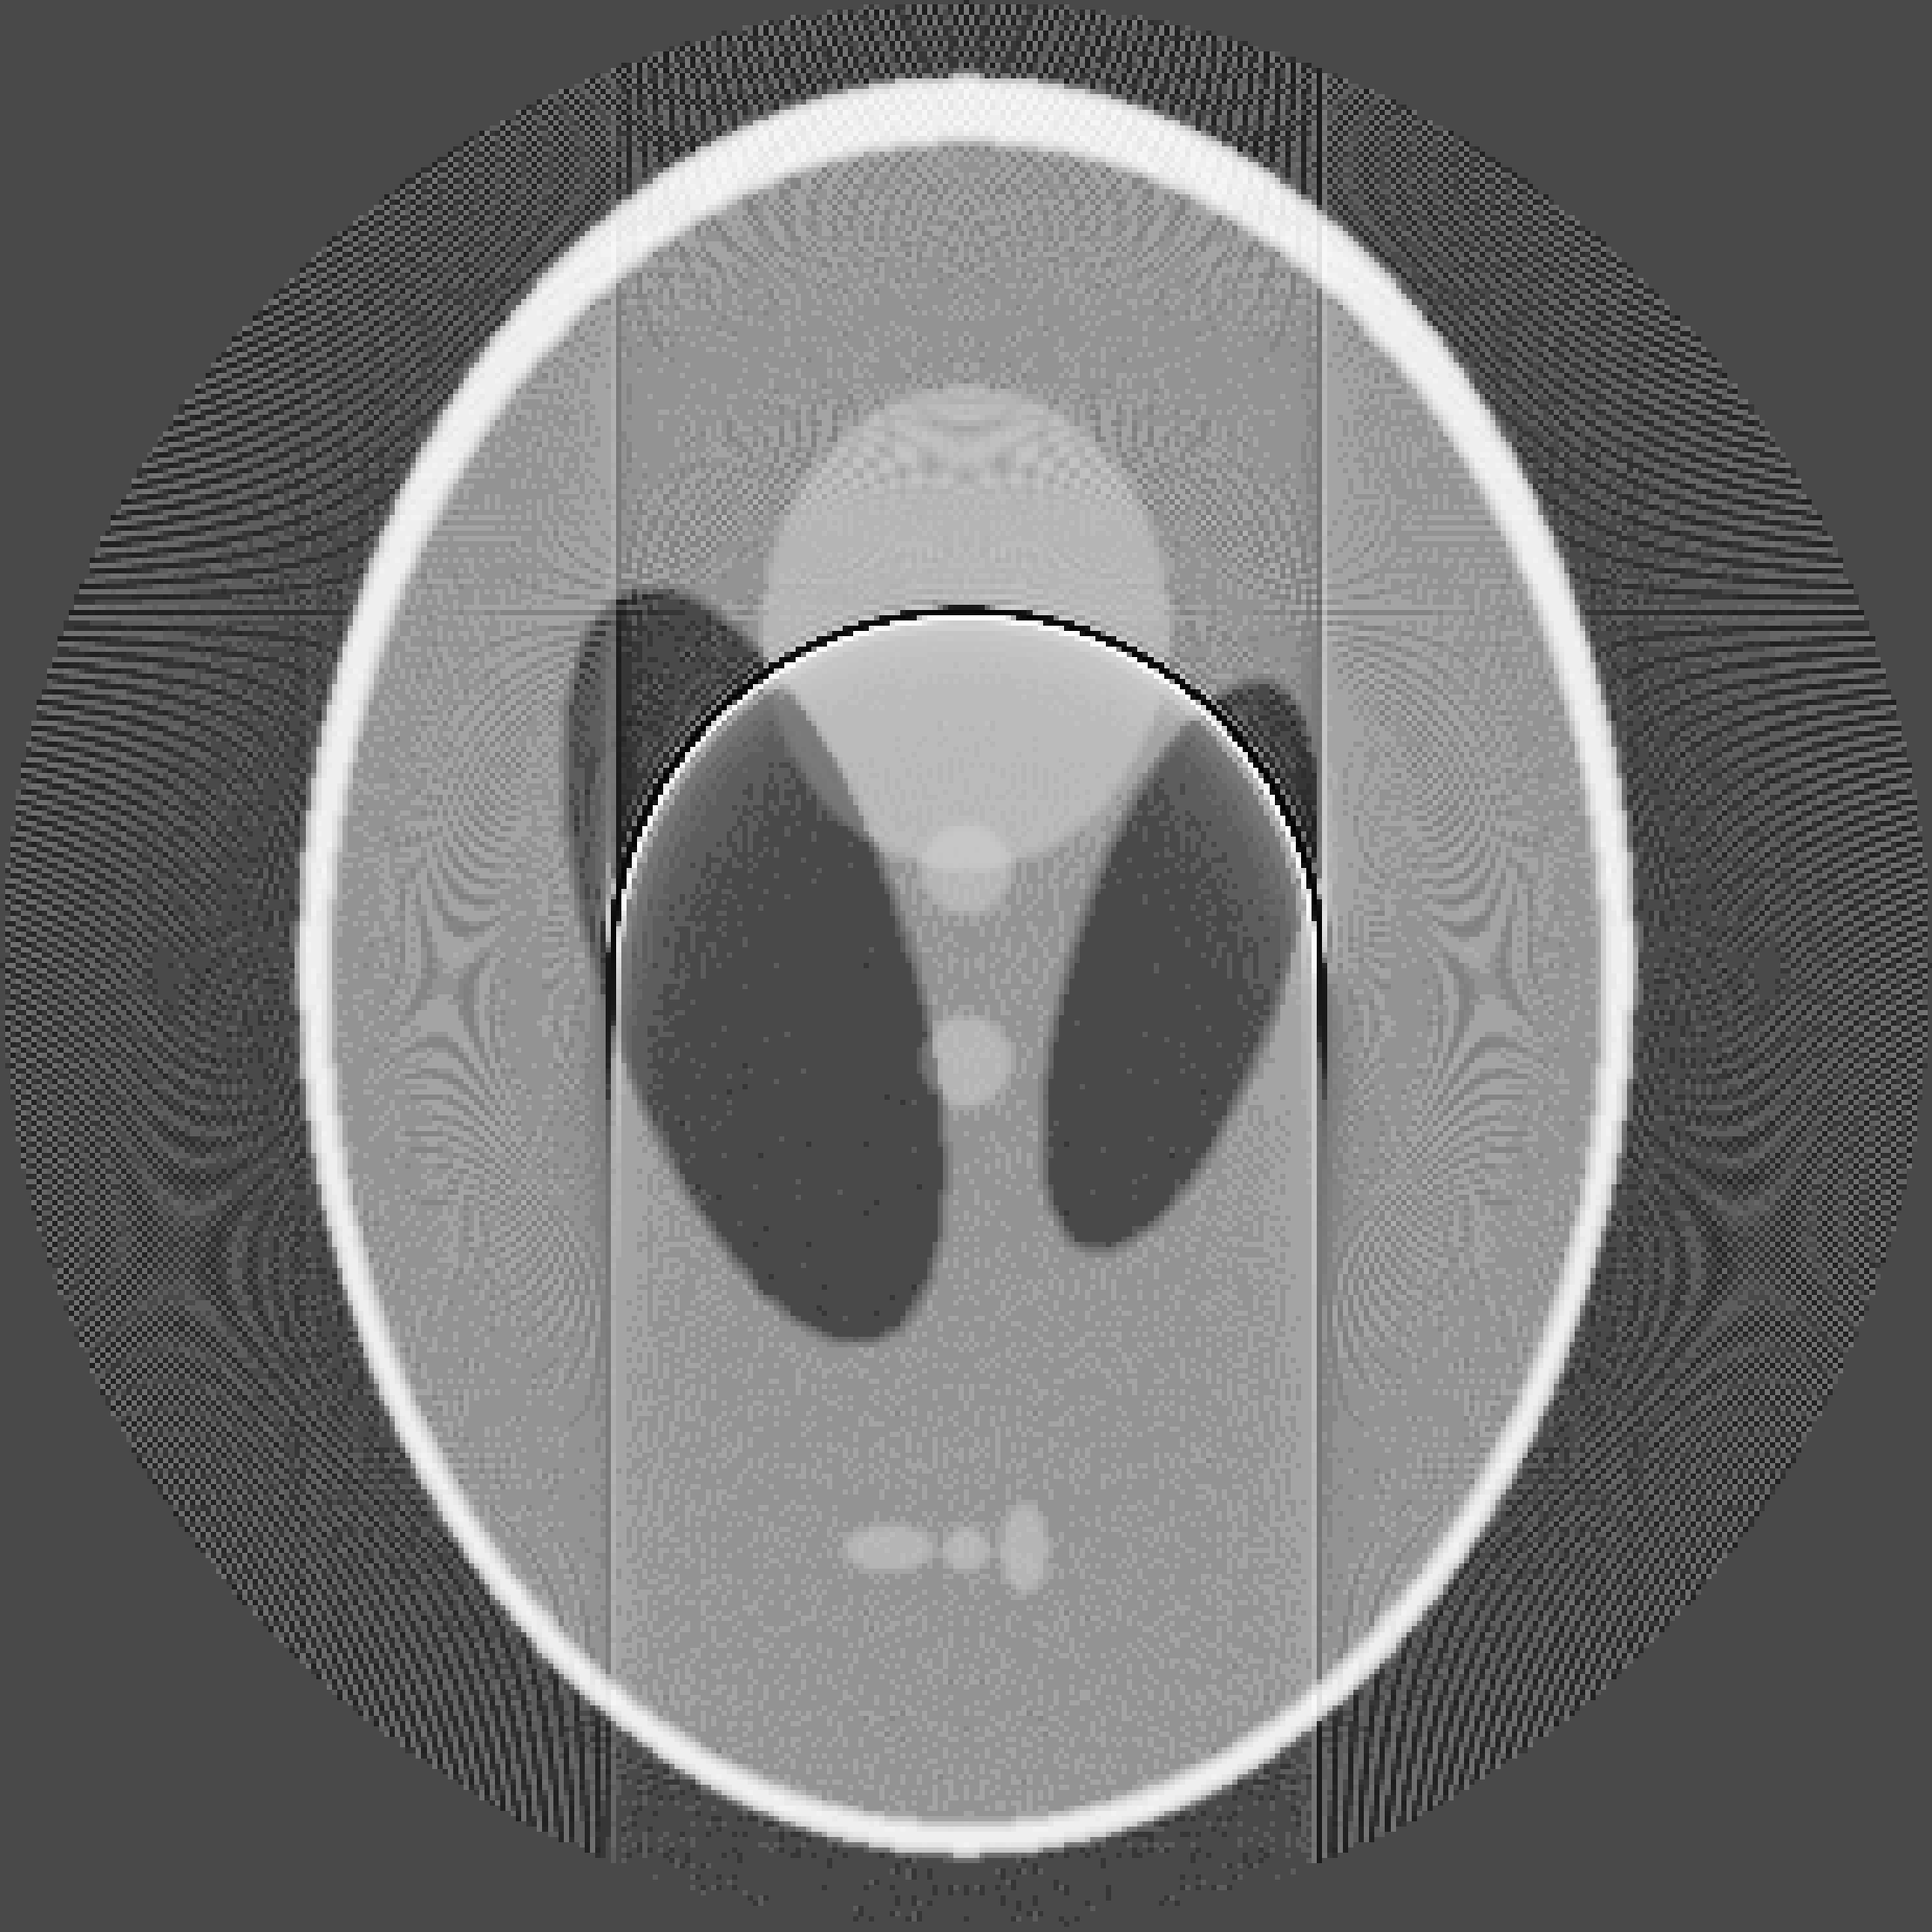
\includegraphics[width=\textwidth]{Figuras/reconstruction_250_EQ.png}
           \caption{Detector 250 defectuoso.}
           \label{fig:sinograma_250} 
        \end{subfigure}
        \begin{subfigure}[h]{0.24\textwidth}
           \centering
           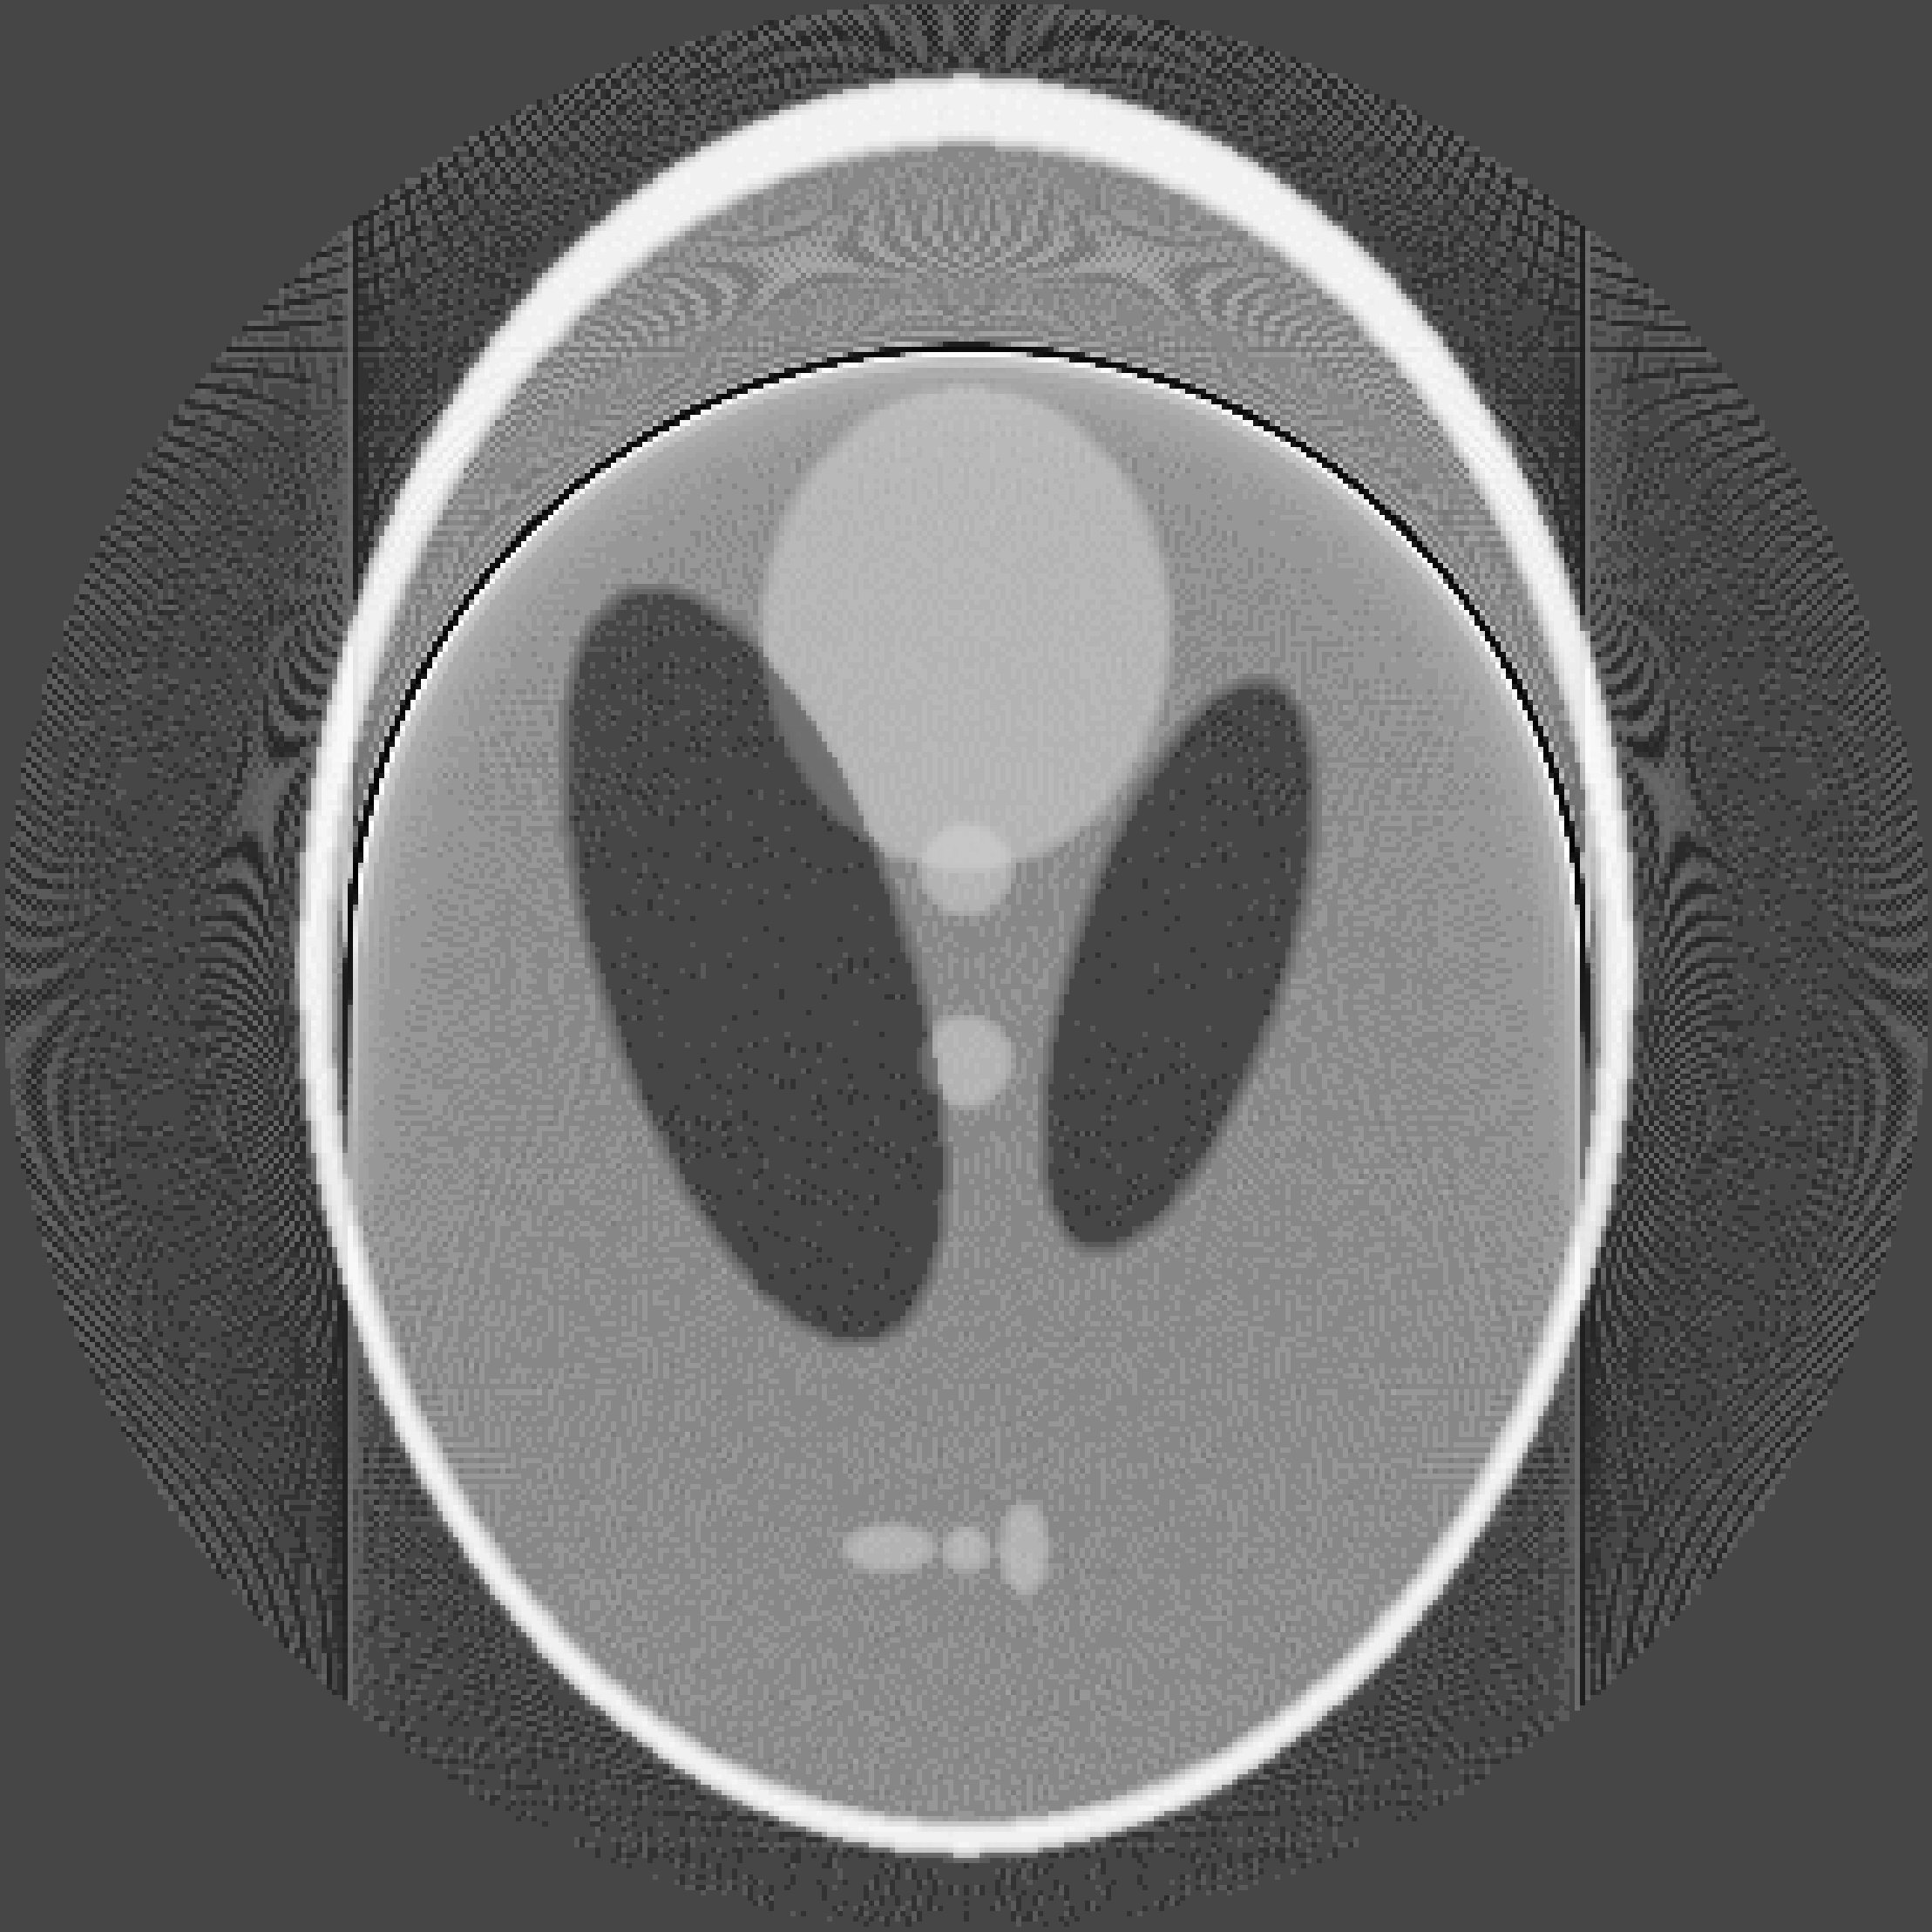
\includegraphics[width=\textwidth]{Figuras/reconstruction_300_EQ.png}
           \caption{Detector 300 defectuoso.}
           \label{fig:sinograma_300} 
        \end{subfigure}
   \caption{Sinogramas generados con 367 detectores y 320 proyecciones. Arriba: Sinogramas con defectos en los detectores 50, 150, 250 y 300 que no registran actividad. Abajo: Retroproyección con filtro rampa de los sinogramas con defectos, estas imágenes fueron ecualizadas.}
   \label{fig:detector_roto}
\end{figure}

Por último, si el sinograma se genera recorriendo la circunferencia completa, el resultado defecto es un círculo completo con cuatro líneas tangentes al círculo. En la Fig. \ref{fig:comp_defecto} se muestra la comparación entre las retroproyecciones filtradas a partir de un sinograma obtenido recorriendo una circunferencia completa y media circunferencia para un equipo que no registra actividad en el detector 150.


\begin{figure}[H]
   \centering
        \begin{subfigure}[h]{0.49\linewidth}
           \centering
           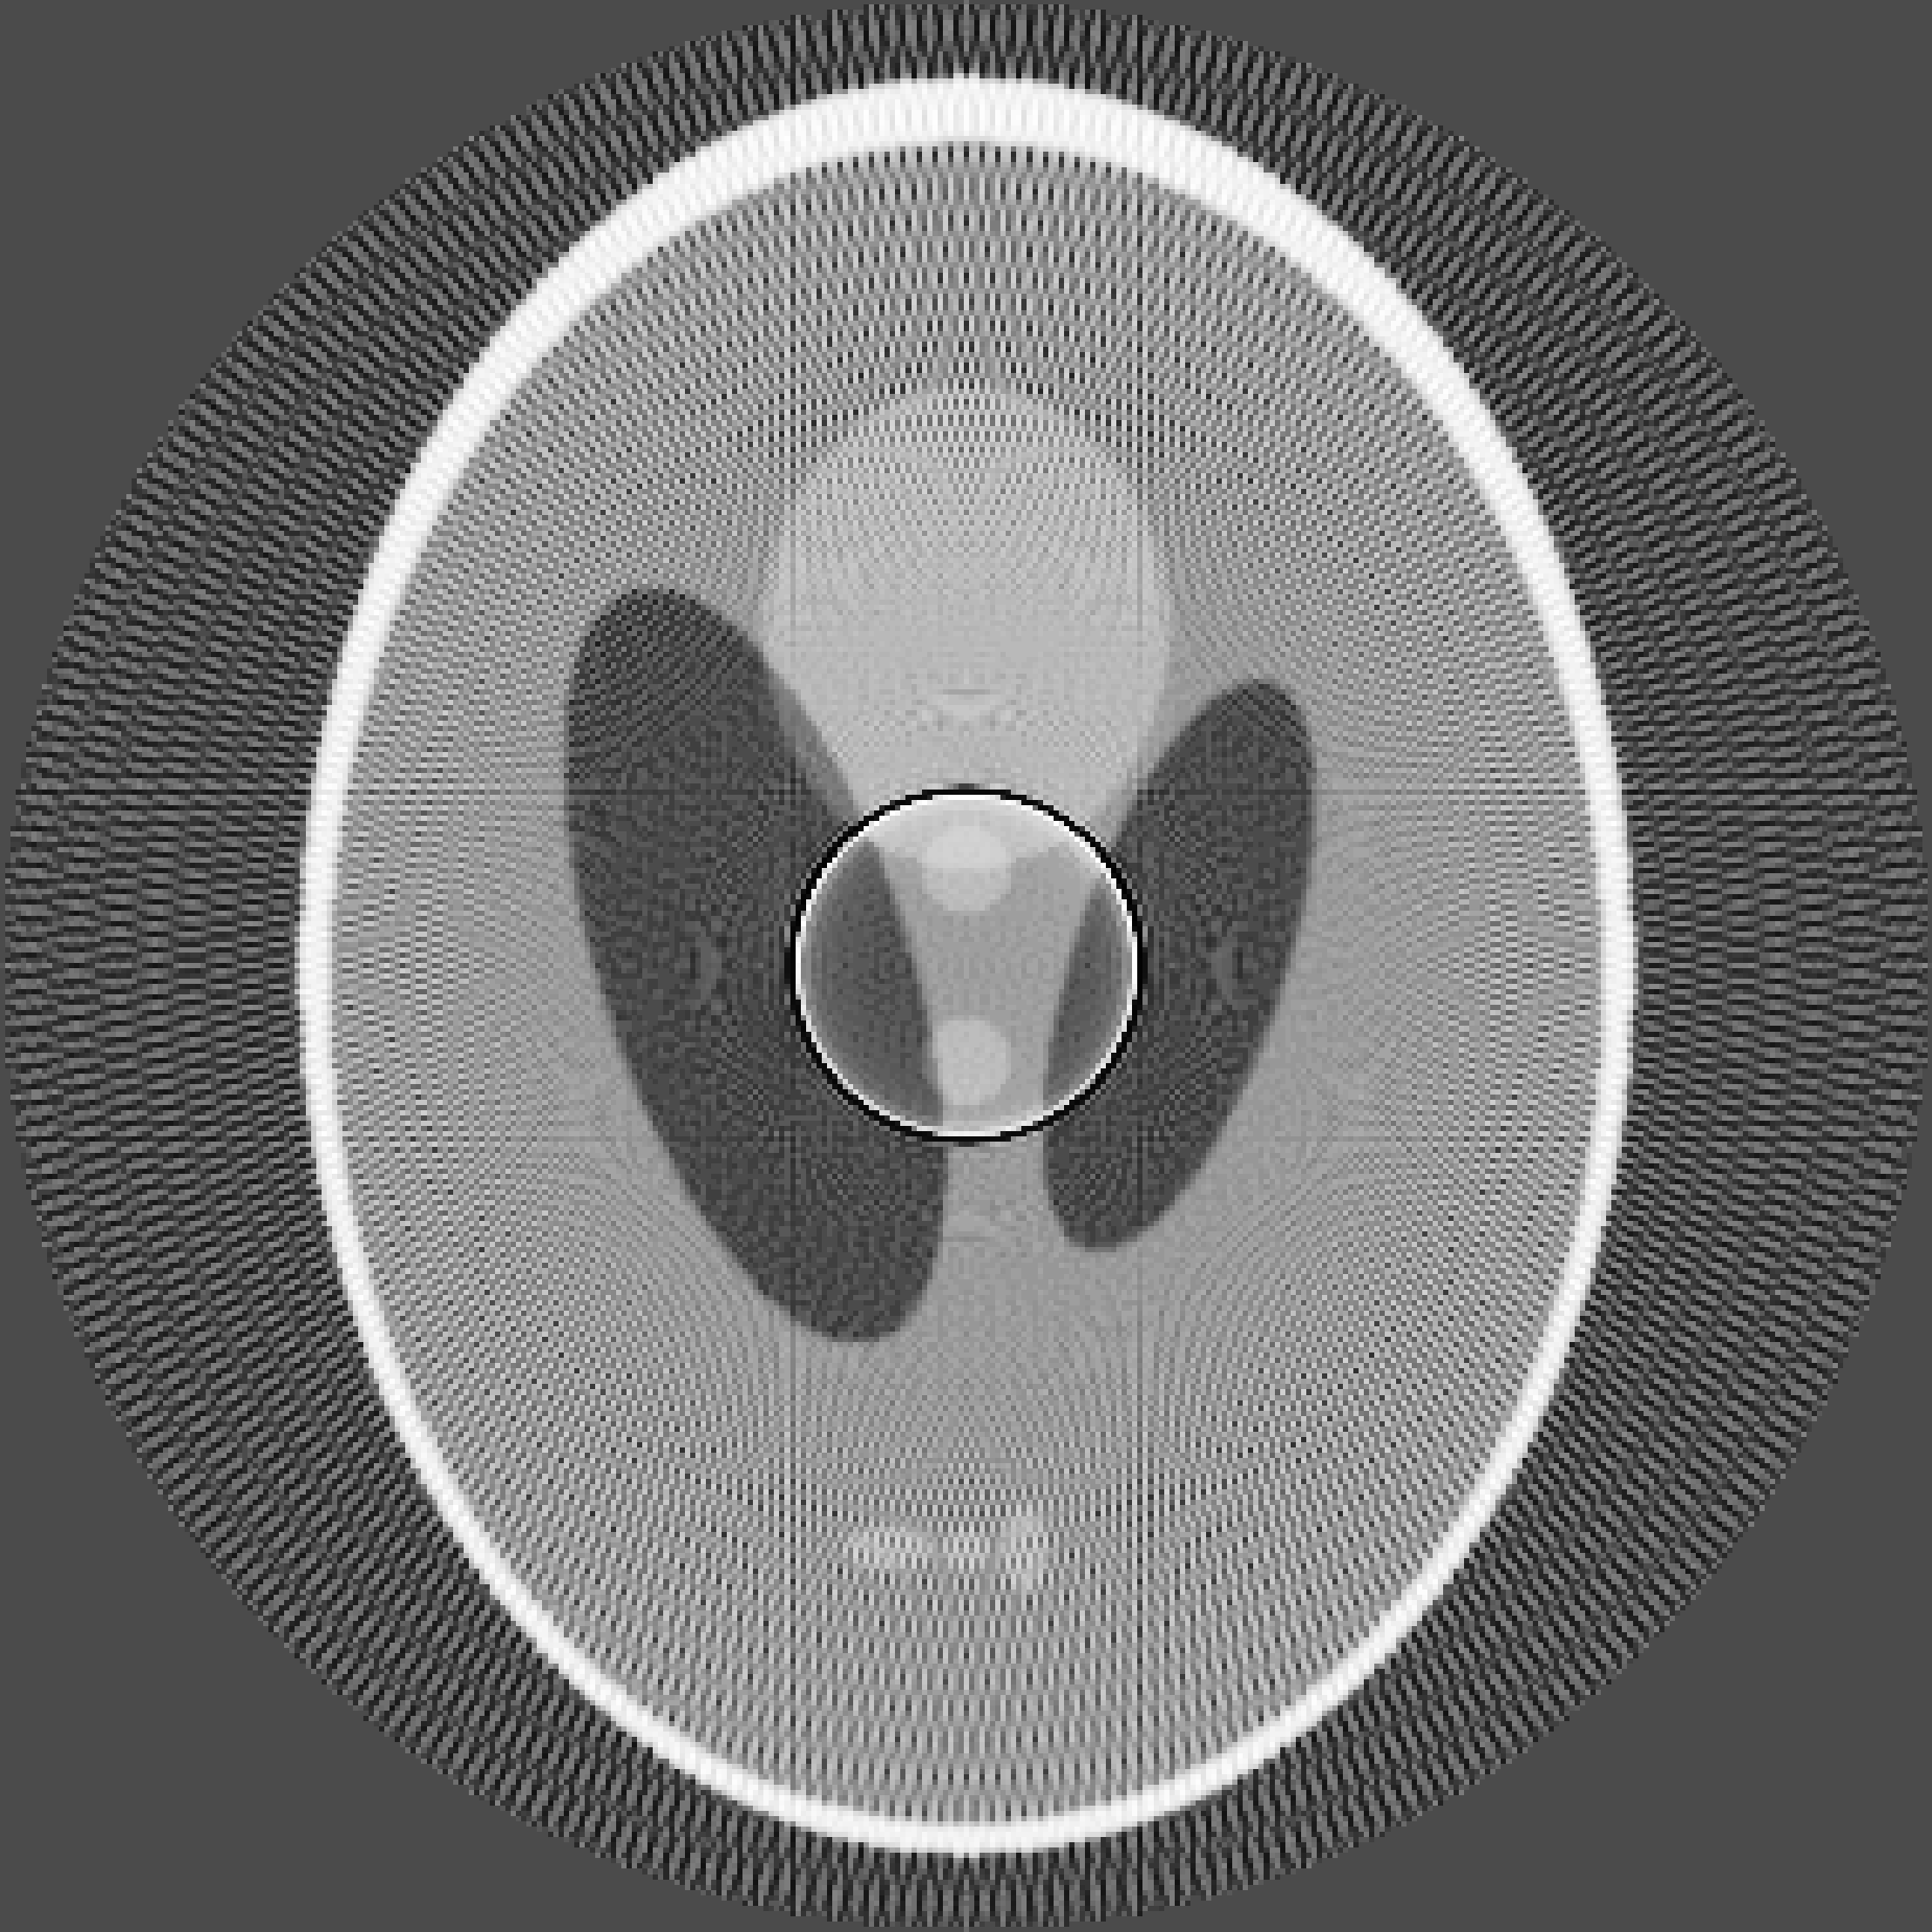
\includegraphics[width=0.8\textwidth]{Figuras/reconstruction_150_360_EQ.png}
           \caption{Sinograma de circunferencia completa.} 
           \label{fig:defecto_360}
        \end{subfigure}
        \begin{subfigure}[h]{0.49\linewidth}
           \centering
           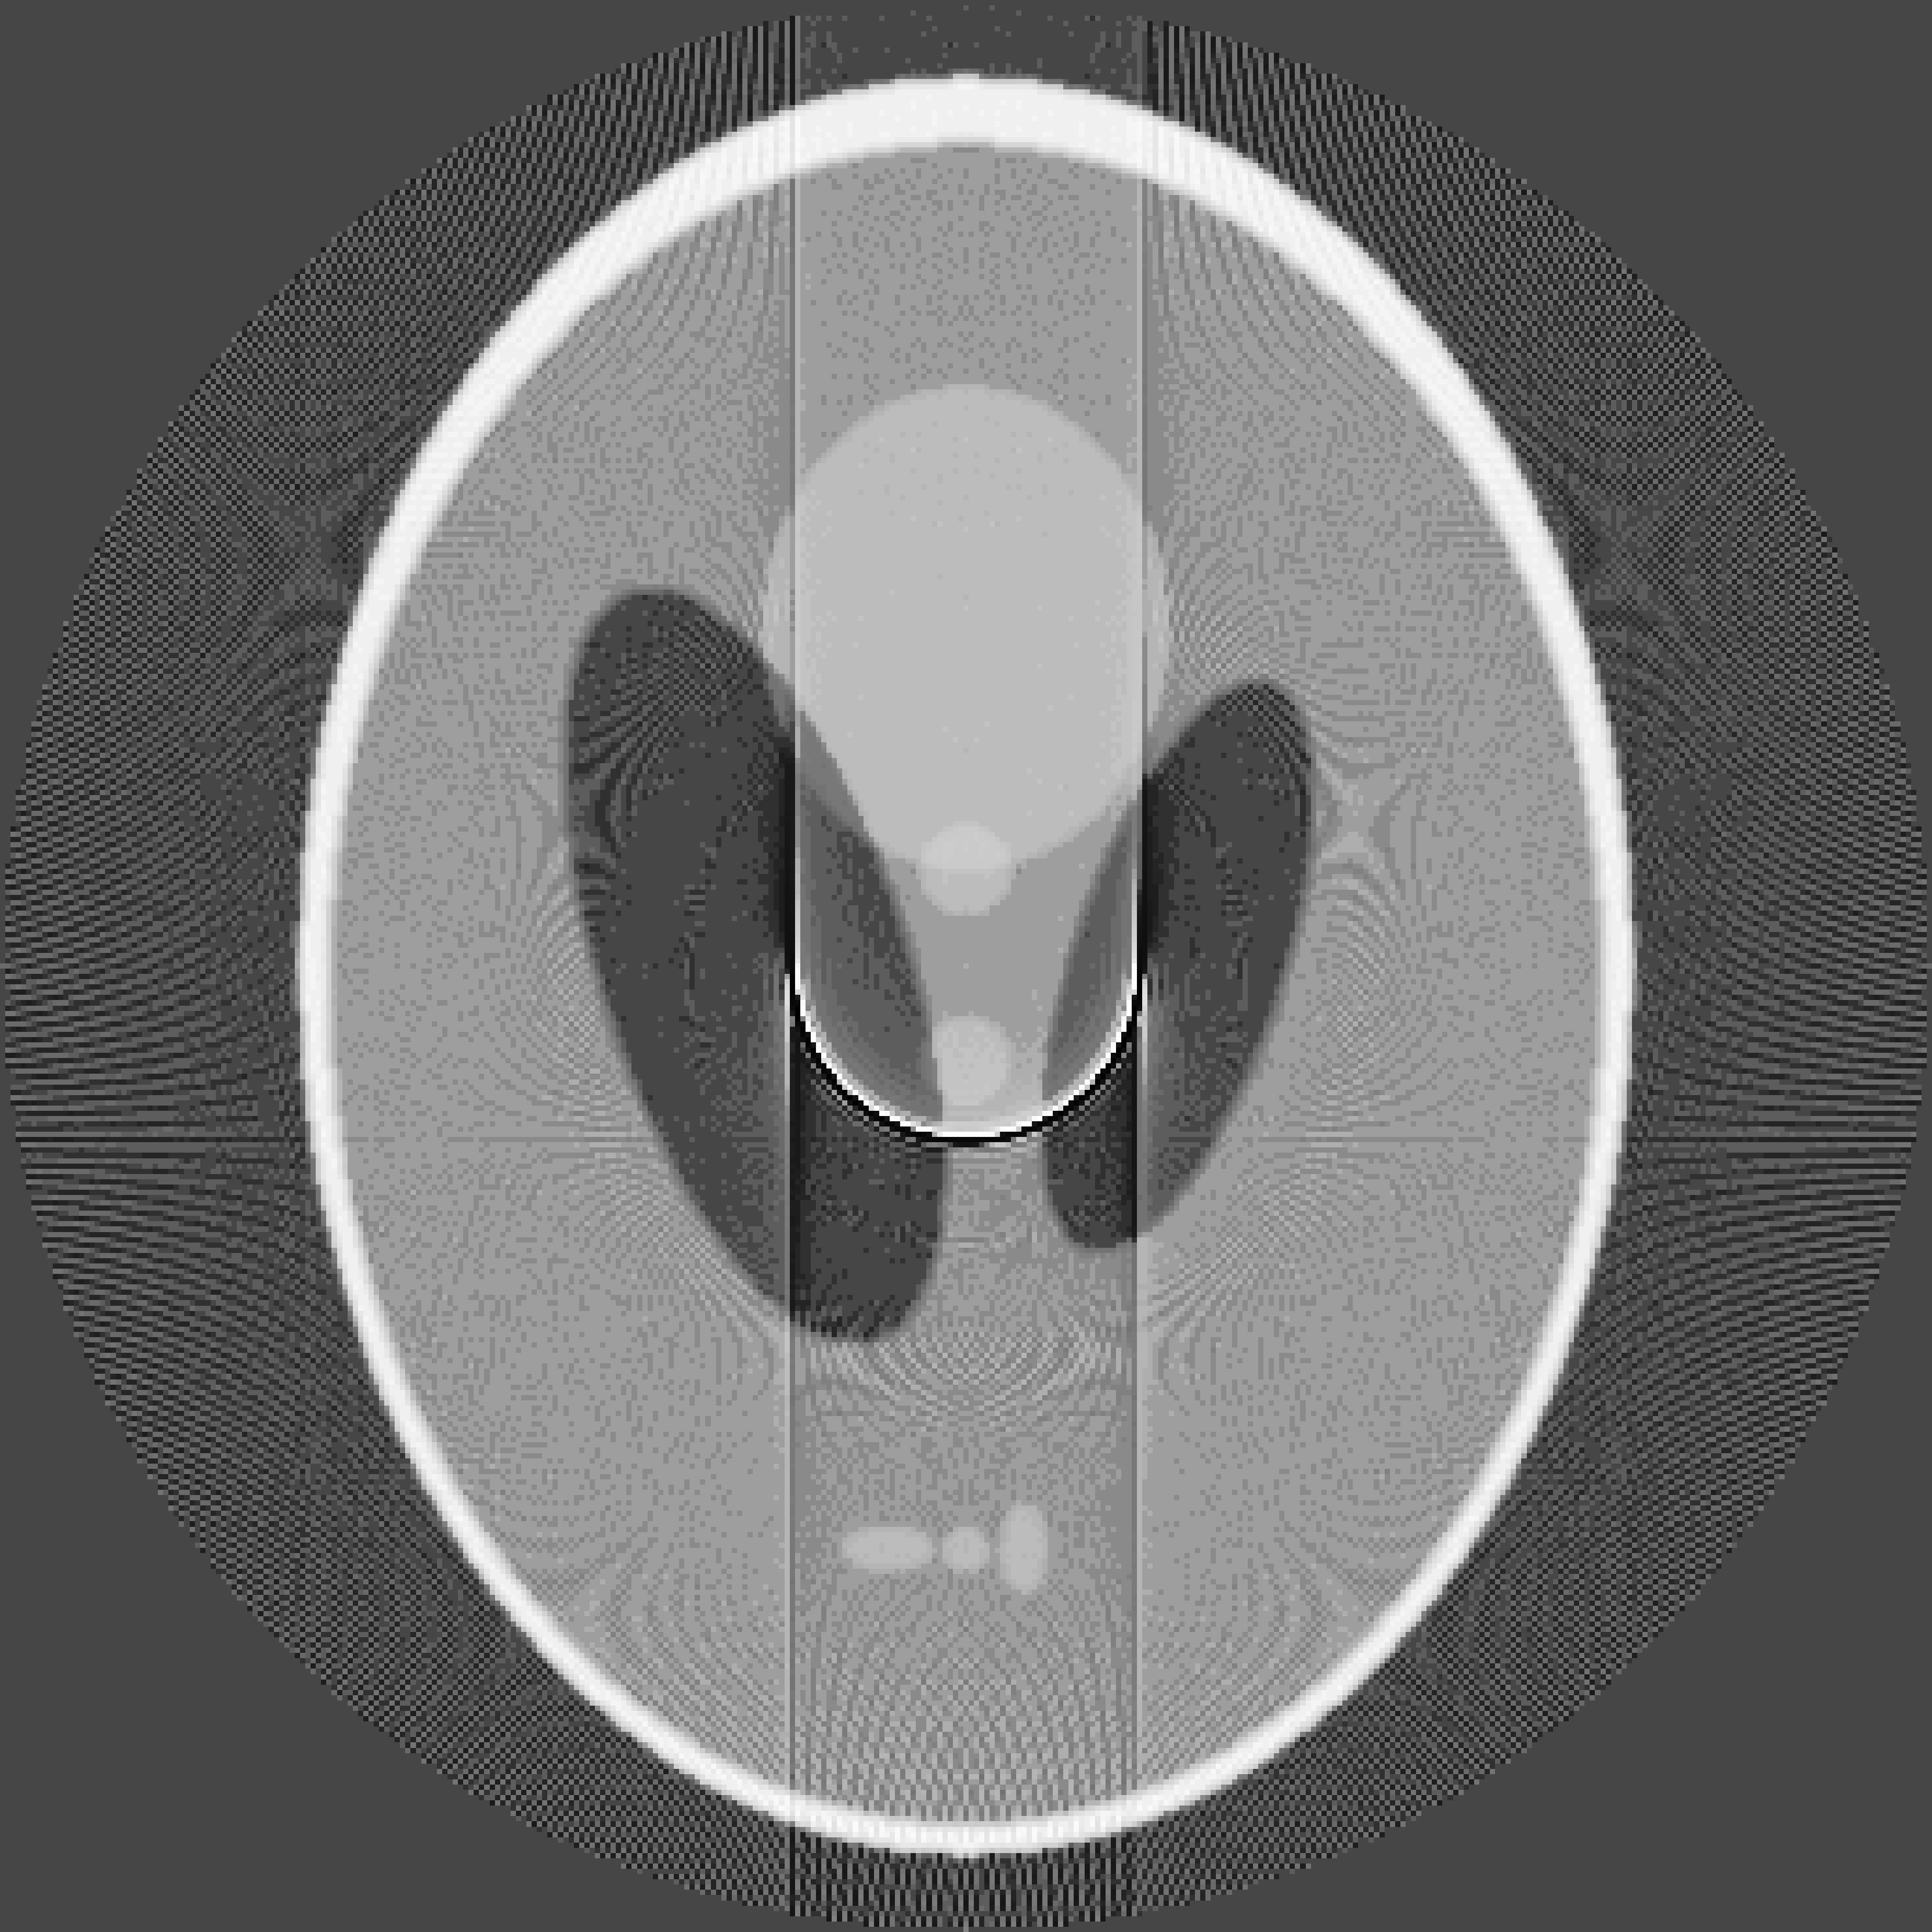
\includegraphics[width=0.8\textwidth]{Figuras/reconstruction_150_EQ.png}
           \caption{Sinograma de media circunferencia.}
           \label{fig:defecto_180}
        \end{subfigure}
   \caption{Comparación entre las retroproyecciones filtradas a partir de un sinograma obtenido recorriendo una circunferencia completa (a) y media circunferencia (b). Imágenes ecualizadas.}
   \label{fig:comp_defecto}
\end{figure}

\centerline{\rule{0.95\linewidth}{0.6pt}}

%\bibliographystyle{plain} % Estilo de bibliografía
%\bibliography{bibliography}    % Nombre de tu archivo .bib sin la extensión

\end{document}